%%%%%%%%%%%%%%%%%%%%%%%%%%%%%%%%%%%%%%%%%%%%%%%%%%%%%%%%%%%%%%%%%%%%%%%%
% Documento di Specifica dei Requisiti Software (SRS) per BugBoard26
% Versione 2.0 — Conforme IEEE 830-1998
% Struttura Modulare
%%%%%%%%%%%%%%%%%%%%%%%%%%%%%%%%%%%%%%%%%%%%%%%%%%%%%%%%%%%%%%%%%%%%%%%%

\documentclass[12pt,a4paper]{article}

% --- PACCHETTI DI BASE ---
\usepackage[utf8]{inputenc}
\usepackage[T1]{fontenc}
\usepackage[italian]{babel}
\usepackage{geometry}
\geometry{a4paper,top=3cm,bottom=3cm,left=2.5cm,right=2.5cm,headheight=16pt}
\usepackage{graphicx}
\usepackage[hidelinks,pdfencoding=auto]{hyperref}
\usepackage{array}
\usepackage{booktabs}
\usepackage{longtable}
\usepackage{tabularx}
\usepackage{ltablex}
\keepXColumns
\usepackage{fancyhdr}
\usepackage{lastpage}
\usepackage{xcolor}
\usepackage{caption}
\usepackage{multirow}
\usepackage{float}
\usepackage{microtype}
\usepackage{enumitem}
\usepackage{titlesec}
\usepackage{tocloft}
\usepackage{FiraSans}
\usepackage{setspace}
\usepackage{needspace}

% --- SIMBOLI CHECK E CROCE PER TABELLE ---
\usepackage{pifont}
\newcommand{\cmark}{\ding{51}}  % checkmark
\newcommand{\xmark}{\ding{55}}  % x mark
\newcommand{\reqseparator}{\vspace{0.3cm}\noindent{\color{bb-outline}\rule{\textwidth}{0.5pt}}\vspace{0.3cm}}

% --- FONT E INTERLINEA ---
\renewcommand{\familydefault}{\sfdefault}
\sffamily
\onehalfspacing

% --- DISABILITA INDENTAZIONE PARAGRAFI ---
\setlength{\parindent}{0pt}
\setlength{\parskip}{0.5em}

% --- COLORI ---
\definecolor{bb-primary}{HTML}{4A55A2}
\definecolor{bb-secondary}{HTML}{7F5283}
\definecolor{bb-surface}{HTML}{F7F2FA}
\definecolor{bb-outline}{HTML}{79747E}
\definecolor{bb-on-surface}{HTML}{1D1B20}
\definecolor{bb-success}{HTML}{4CAF50}
\definecolor{bb-warning}{HTML}{FFC107}
\definecolor{bb-error}{HTML}{F44336}

% --- MACRO ---
\newcommand{\productname}{BugBoard26}

% --- STILI TITOLI ---
\titleformat{\subsection}{\Large\bfseries\color{bb-primary}}{\thesubsection}{1em}{}
\titleformat{\subsubsection}{\large\bfseries\color{bb-secondary}}{\thesubsubsection}{1em}{}
\titleformat{\paragraph}{\bfseries\color{bb-on-surface}}{\theparagraph}{1em}{}
\titleformat{\subparagraph}{\bfseries\color{bb-on-surface}}{\thesubparagraph}{1em}{}
\titlespacing{\subparagraph}{0pt}{*1}{*0.5}
\setcounter{secnumdepth}{4}
\setcounter{tocdepth}{3}

% --- BOX STILISTICI ---
\usepackage[most]{tcolorbox}
\newtcolorbox{mainbox}[1][]{
    colback=bb-surface,
    colframe=bb-primary!80!black,
    coltitle=white,
    colbacktitle=bb-primary,
    fonttitle=\bfseries\large,
    boxrule=1pt,
    arc=5mm,
    boxsep=5mm,
    breakable,
    #1
}

\newtcolorbox{ucbox}[1][]{
    colback=white,
    colframe=bb-outline,
    coltitle=bb-on-surface,
    colbacktitle=bb-surface,
    fonttitle=\bfseries,
    boxrule=0.5pt,
    arc=4mm,
    boxsep=4mm,
    breakable,
    #1
}

% --- BOX PER REQUISITI FUNZIONALI ---
\newtcolorbox{reqbox}[1][]{
    colback=bb-surface!30,
    colframe=bb-primary!50,
    coltitle=bb-primary,
    fonttitle=\bfseries\large,
    boxrule=0.8pt,
    arc=3mm,
    left=8pt,
    right=8pt,
    top=8pt,
    bottom=8pt,
    breakable,
    enhanced,
    attach boxed title to top left={yshift=-2mm, xshift=5mm},
    boxed title style={
        colback=bb-primary!10,
        colframe=bb-primary!50,
        arc=2mm,
        boxrule=0.5pt
    },
    #1
}

% --- HEADER E FOOTER ---
\pagestyle{fancy}
\fancyhf{}
\fancyhead[L]{\textcolor{bb-outline}{\bfseries \productname} - Specifica dei Requisiti}
\fancyfoot[C]{\textcolor{bb-outline}{Pagina \thepage\ di \pageref{LastPage}}}
\fancyfoot[R]{\textcolor{bb-outline}{Versione 1.0}}
\renewcommand{\headrulewidth}{0.4pt}
\renewcommand{\footrulewidth}{0.4pt}
\definecolor{rulecolor}{HTML}{79747E}
\renewcommand{\headrule}{\color{rulecolor}\hrule}
\renewcommand{\footrule}{\color{rulecolor}\hrule}

% --- RIDEFINISCI STILE PLAIN (usato da \tableofcontents e prima pagina sezioni) ---
\fancypagestyle{plain}{
  \fancyhf{}
  \fancyhead[L]{\textcolor{bb-outline}{\bfseries \productname} - Specifica dei Requisiti}
  \fancyfoot[C]{\textcolor{bb-outline}{Pagina \thepage\ di \pageref{LastPage}}}
  \fancyfoot[R]{\textcolor{bb-outline}{Versione 1.0}}
  \renewcommand{\headrulewidth}{0.4pt}
  \renewcommand{\footrulewidth}{0.4pt}
  \renewcommand{\headrule}{\color{rulecolor}\hrule}
  \renewcommand{\footrule}{\color{rulecolor}\hrule}
}

% --- STILE PAGINA FRONTESPIZIO (nessun header/footer) ---
\fancypagestyle{frontespizio}{
  \fancyhf{}
  \renewcommand{\headrulewidth}{0pt}
  \renewcommand{\footrulewidth}{0pt}
}

% --- CONFIGURAZIONE SPAZIATURA INDICE ---
\setlength{\cftbeforesubsecskip}{0.4em}
\setlength{\cftbeforesubsubsecskip}{0.2em}
\setlength{\cftbeforeparaskip}{0.1em}

% --- INDICE PERSONALIZZATO ---
\renewcommand{\cftsubsecleader}{\cftdotfill{\cftdotsep}}
\renewcommand{\cftsubsecfont}{\bfseries}
\renewcommand{\cftsubsubsecfont}{\mdseries}

% --- INIZIO DOCUMENTO ---
\begin{document}

% --- FRONTESPIZIO (senza numerazione né header/footer) ---
\pagenumbering{gobble}
\begin{titlepage}
\thispagestyle{empty}
\newgeometry{left=2.5cm,right=2.5cm,top=2cm,bottom=2cm}

\begin{center}

\includegraphics[width=0.5\textwidth]{UNINA.png}
\end{center}

\begin{center}
{\color{bb-primary}\Huge\bfseries \productname\par}
\end{center}

\begin{center}
{\color{bb-on-surface}\LARGE\bfseries Documentazione BugBoard26\par}
{\large\color{bb-outline} (BugBoard26 Documentation)}
\end{center}

\vfill

\begin{tcolorbox}[
    colback=bb-surface,
    colframe=bb-outline!30,
    boxrule=1pt,
    arc=8mm,
    boxsep=8mm,
    width=0.9\textwidth,
    center
]

\large
\begin{tabularx}{\linewidth}{@{} >{\itshape}l X >{\itshape}r @{}}
Antonio Scafaro & & N86005219 \\
Alessio Paduano & & N86005142 \\
Luigi Pio Scalice & & N86005197 \\
\end{tabularx}


\end{tcolorbox}

\vfill

\begin{center}
\color{bb-outline}
\rule{0.7\textwidth}{0.4pt}\par
\vspace{0.4cm}
{\large Corso di Ingegneria del Software \par}
{\large A.A. 2025/2026}
\end{center}

\restoregeometry
\end{titlepage}


% --- INDICE (numerazione romana i, ii, iii...) ---
\pagenumbering{roman}
\setcounter{page}{1}

% Usa geometry più ampia per l'indice
\newgeometry{a4paper,top=3cm,bottom=4cm,left=2.5cm,right=2.5cm,headheight=16pt,footskip=1.5cm}

\tableofcontents

% Ripristina geometry normale
\restoregeometry

\clearpage

% --- INIZIO CONTENUTO (numerazione araba 1, 2, 3...) ---
\pagenumbering{arabic}
\setcounter{page}{1}

\section{Analisi dei requisiti}
% ---------------------------------------------------------------------
% SEZIONE 1: INTRODUZIONE (IEEE 830-1998)
% ---------------------------------------------------------------------
% ---------------------------------------------------------------------
\subsection{Introduzione}
\label{sec:introduzione}
% ---------------------------------------------------------------------

Questo documento rappresenta la Specifica dei Requisiti Software (SRS) per il sistema \productname, un'applicazione per la gestione collaborativa di issue in progetti software. Il documento è conforme allo standard IEEE 830-1998.

% ---------------------------------------------------------------------
\subsubsection{Scopo}
\label{subsec:scopo}
% ---------------------------------------------------------------------

Lo scopo di questo documento è fornire una specifica completa, accurata e verificabile dei requisiti funzionali e non funzionali del sistema \productname. Questo SRS è destinato ai seguenti stakeholder:

\begin{itemize}[leftmargin=1.1em]
\item \textbf{Team di sviluppo}: per comprendere nel dettaglio le funzionalità da implementare e i vincoli da rispettare.
\item \textbf{Project manager}: per pianificare attività, risorse e tempistiche di sviluppo.
\item \textbf{Quality Assurance}: per definire criteri di accettazione e test plan.
\item \textbf{Committente}: per validare che i requisiti soddisfino le esigenze di business.
\end{itemize}

Il documento costituisce la base contrattuale tra il team di sviluppo e il committente (SoftEngUniNA), definendo in modo non ambiguo ciò che il sistema deve fare e come deve comportarsi.

% ---------------------------------------------------------------------
\subsubsection{Ambito del prodotto}
\label{subsec:ambito}
% ---------------------------------------------------------------------

\noindent\textbf{Nome del prodotto}: \productname

\noindent\textbf{Descrizione generale}: \productname{} è una piattaforma distribuita per la gestione collaborativa di issue (segnalazioni) in progetti software. Il sistema consente di:

\begin{itemize}[leftmargin=1.1em]
\item Organizzare il lavoro in progetti distinti, ciascuno con il proprio team
\item Segnalare issue (bug, feature, domande, documentazione) all'interno dei progetti autorizzati
\item Monitorare lo stato di avanzamento delle issue attraverso workflow configurabili
\item Assegnare issue a membri del team del progetto
\item Collaborare tramite commenti e discussioni
\item Generare report mensili per progetto per analizzare performance del team
\end{itemize}

\noindent\textbf{Gestione Progetti e Permessi}:

Gli amministratori hanno controllo completo su:
\begin{itemize}[leftmargin=1.1em]
\item Creazione, modifica ed eliminazione progetti
\item Assegnazione utenti ai progetti (chi può accedere a cosa)
\item Gestione membri del team per ciascun progetto
\end{itemize}

Gli utenti standard possono:
\begin{itemize}[leftmargin=1.1em]
\item Visualizzare solo i progetti a cui sono stati assegnati dagli amministratori
\item Creare e gestire issue solo all'interno dei progetti a cui hanno accesso
\item Lavorare sulle issue che gli vengono assegnate dagli amministratori
\end{itemize}

\noindent\textbf{Benefici attesi}:

\begin{itemize}[leftmargin=1.1em]
\item Miglioramento della tracciabilità dei problemi e delle richieste
\item Riduzione del tempo medio di risoluzione grazie a una migliore organizzazione
\item Aumento della trasparenza e della collaborazione all'interno del team
\item Supporto decisionale attraverso analisi quantitative delle performance
\end{itemize}

\noindent\textbf{Obiettivi principali}:

\begin{itemize}[leftmargin=1.1em]
\item Fornire un sistema performante (tempo di risposta $\leq$ 3000ms per operazioni comuni)
\item Garantire la sicurezza dei dati sensibili attraverso autenticazione robusta
\item Assicurare l'usabilità con un'interfaccia intuitiva che richieda training minimo
\item Facilitare la manutenibilità attraverso un'architettura distribuita e modulare
\end{itemize}

\noindent\textbf{Cosa NON è incluso nell'ambito}:

\begin{itemize}[leftmargin=1.1em]
\item Integrazione con sistemi di versionamento del codice (Git, SVN)
\item Funzionalità di continuous integration/deployment
\end{itemize}

% ---------------------------------------------------------------------
\subsubsection{Definizioni, acronimi e abbreviazioni}
\label{subsec:definizioni}
% ---------------------------------------------------------------------

Per una trattazione completa dei termini specifici del dominio, degli acronimi e delle abbreviazioni utilizzati in questo documento, si rimanda alla Sezione~\ref{sec:glossario} (Glossario).

Alcuni termini chiave includono:

\begin{itemize}[leftmargin=1.1em]
\item \textbf{Issue}: segnalazione relativa al progetto (bug, feature, question, documentation)
\item \textbf{BE}: Back-end, componente server-side del sistema
\item \textbf{FE}: Front-end, componente client-side del sistema
\item \textbf{API}: Application Programming Interface, interfaccia REST per la comunicazione BE-FE
\end{itemize}

% ---------------------------------------------------------------------
\subsubsection{Riferimenti}
\label{subsec:riferimenti}
% ---------------------------------------------------------------------

Questo documento fa riferimento ai seguenti standard, specifiche e documenti tecnici:

\begin{longtable}{p{0.15\linewidth} p{0.78\linewidth}}
\toprule
\textbf{Rif.} & \textbf{Descrizione} \\
\midrule
\endhead
\bottomrule
\endfoot

RIF-1 & \textit{Progetto-SWE-2025-2026 - canale 2\_v1.pdf}. Specifica del committente con requisiti di alto livello e vincoli del progetto. \\
\addlinespace

RIF-2 & \textit{IEEE Std 830-1998: IEEE Recommended Practice for Software Requirements Specifications}. Standard di riferimento per la struttura e il contenuto di documenti SRS. \\
\addlinespace

RIF-3 & \textit{Cockburn, A. (2000). Writing Effective Use Cases}. Metodologia per la descrizione testuale strutturata di casi d'uso. \\
\addlinespace

\end{longtable}

\newpage

% ---------------------------------------------------------------------
\subsection{Panoramica del documento}
\label{subsec:panoramica}
% ---------------------------------------------------------------------

Il presente documento è organizzato come segue:

\begin{itemize}[leftmargin=1.1em]
\item \textbf{Sezione~\ref{sec:introduzione} -- Introduzione}: fornisce una panoramica del documento, descrive lo scopo del sistema, definisce gli acronimi e elenca i riferimenti normativi e bibliografici.

\item \textbf{Sezione~\ref{sec:glossario} -- Glossario}: contiene le definizioni di tutti i termini tecnici, gli acronimi e i riferimenti utilizzati nel documento per evitare ambiguità.

\item \textbf{Sezione~\ref{sec:casi-uso} -- Casi d'Uso}: presenta il diagramma UML dei casi d'uso e la lista completa delle funzionalità del sistema, modellando le interazioni tra gli attori e il sistema.

\item \textbf{Sezione~\ref{sec:caratterizzazione-utenti} -- Caratterizzazione Utenti}: identifica e descrive in dettaglio i profili degli utenti del sistema (Utente, Utente Autenticato, Amministratore), specificandone obiettivi, responsabilità e permessi.

\item \textbf{Sezione~\ref{sec:requisiti-specifici} -- Requisiti Specifici}: costituisce il cuore tecnico del documento e include:
  \begin{itemize}
  \item \textbf{Requisiti di Sistema}: vincoli architetturali e di sistema imposti dal committente
  \item \textbf{Requisiti Funzionali}: descrizione dettagliata di tutte le funzionalità assegnate
  \item \textbf{Requisiti Non Funzionali}: requisiti di qualità misurabili e verificabili (usabilità, performance, sicurezza, manutenibilità, affidabilità)
  \end{itemize}

\item \textbf{Sezione~\ref{sec:cockburn} -- Descrizione Dettagliata Casi d'Uso}: fornisce la formalizzazione testuale strutturata secondo il template di Cockburn per un caso d'uso significativo.

\item \textbf{Sezione~\ref{sec:mockup} -- Mockup}: presenta la prototipazione visuale delle interfacce utente per i casi d'uso formalizzati, collegata agli step delle tabelle Cockburn.
\end{itemize}

Questo documento deve essere letto in modo sequenziale al primo approccio. Le sezioni successive possono essere consultate in modo non lineare come riferimento durante le fasi di progettazione, implementazione e testing.

\newpage

% ---------------------------------------------------------------------
% SEZIONE 2: GLOSSARIO
% ---------------------------------------------------------------------
% ---------------------------------------------------------------------
\subsection{Glossario}
\label{sec:glossario}
% ---------------------------------------------------------------------

\subsubsection{Termini del dominio}
\label{subsec:termini-dominio}

\begin{ucbox}[title=Glossario dei Termini]
\begin{longtable}{p{0.25\linewidth} p{0.68\linewidth}}
\toprule
\textbf{Termine} & \textbf{Descrizione} \\
\midrule
\endhead
\bottomrule
\endfoot

\textbf{Account} & Insieme di informazioni e credenziali (email, password) che identificano univocamente un utente e ne regolano l'accesso al sistema. \\
\addlinespace

\textbf{Amministratore} & Utente con ruolo privilegiato che possiede tutti i permessi di un utente autenticato, più funzionalità aggiuntive di gestione del sistema (creazione utenze, assegnazione issue, archiviazione, accesso ai report). \\
\addlinespace

\textbf{Archiviazione} & Operazione riservata agli Amministratori che sposta una issue in una sezione di archivio, rimuovendola dalle liste principali ma mantenendone l'accessibilità da una vista dedicata. \\
\addlinespace

\textbf{Assegnazione} & Operazione con cui un Amministratore associa una issue a un membro specifico del team, rendendolo responsabile della sua gestione. \\
\addlinespace

\textbf{Autenticazione} & Processo di verifica dell'identità di un utente tramite credenziali (email e password) per consentire l'accesso alle funzionalità del sistema. \\
\addlinespace

\textbf{Bug} & Tipo di issue che descrive un errore, difetto o malfunzionamento del software rispetto al comportamento atteso. \\
\addlinespace

\textbf{Commento} & Messaggio testuale lasciato da un utente autenticato all'interno della sezione di discussione di una issue specifica. \\
\addlinespace

\textbf{Dashboard} & Pagina principale visualizzata dopo il login, che fornisce una panoramica delle issue e delle attività rilevanti per l'utente. \\
\addlinespace

\textbf{Documentation} & Tipo di issue che segnala problemi, mancanze o necessità di chiarimenti nella documentazione del progetto. \\
\addlinespace

\textbf{Etichetta (Label)} & Marcatore testuale personalizzabile associabile a una issue per facilitarne la categorizzazione, il filtraggio e la ricerca (es. "frontend", "urgente", "sicurezza"). \\
\addlinespace

\textbf{Feature} & Tipo di issue che rappresenta la richiesta di una nuova funzionalità o un miglioramento del sistema esistente. \\
\addlinespace

\textbf{Filtro} & Criterio di selezione applicabile alla lista delle issue per visualizzare solo quelle che soddisfano specifiche condizioni (es. tipo, stato, priorità). \\
\addlinespace

\textbf{Issue} & Segnalazione relativa al progetto; entità fondamentale del sistema. Può essere di quattro tipi: Bug, Feature, Question, Documentation. Ogni issue ha attributi obbligatori (titolo, descrizione, tipo, priorità, stato) e opzionali (etichette, immagini, assegnatario). \\
\addlinespace

\textbf{Metrica} & Misura quantitativa aggregata utilizzata nei report mensili per valutare performance e attività del team (es. numero di issue aperte, tempo medio di risoluzione). \\
\addlinespace

\textbf{Notifica} & Messaggio informativo inviato automaticamente dal sistema a un utente in seguito a eventi specifici (es. assegnazione di una issue). \\
\addlinespace

\textbf{Ordinamento} & Operazione che modifica la sequenza di visualizzazione delle issue secondo un criterio specificato (es. data di creazione, priorità) e una direzione (crescente o decrescente). \\
\addlinespace

\textbf{Priorità} & Attributo opzionale che definisce il livello di urgenza di una issue. Valori ammessi: Nessuna, Bassa, Media, Alta, Critica. \\
\addlinespace

\textbf{Progetto} & Spazio di lavoro organizzativo che raggruppa un insieme di issue relative a uno specifico prodotto software. \\
\addlinespace

\textbf{Question} & Tipo di issue utilizzato per porre domande o richiedere chiarimenti sul progetto. \\
\addlinespace

\textbf{Report Mensile} & Documento riepilogativo generato automaticamente dal sistema, contenente metriche aggregate sull'attività del team in un intervallo temporale di un mese. Accessibile solo agli Amministratori. \\
\addlinespace

\textbf{Ruolo} & Attributo associato a un account utente che determina l'insieme di permessi e funzionalità accessibili. Valori possibili: Utente (standard) o Amministratore. \\
\addlinespace

\textbf{Stato} & Fase corrente nel ciclo di vita di una issue. Stato iniziale: "ToDo". Altri stati possibili includono: In Lavorazione, Risolta, Chiusa, Archiviata. \\
\addlinespace

\textbf{Team} & Insieme degli utenti che collaborano al progetto utilizzando la piattaforma \productname. \\
\addlinespace

\textbf{ToDo} & Stato iniziale di una issue appena creata, che indica che non è ancora stata presa in carico da alcun membro del team. \\
\addlinespace

\textbf{Utente} & Individuo che interagisce con il sistema. Prima dell'autenticazione, può accedere solo alla schermata di login. \\
\addlinespace

\textbf{Utente Autenticato} & Utente che ha completato con successo il processo di autenticazione e ha accesso alle funzionalità di base del sistema (creazione, visualizzazione e modifica issue, commenti). \\

\end{longtable}
\end{ucbox}

\subsubsection{Acronimi e abbreviazioni}
\label{subsec:acronimi}

\begin{longtable}{p{0.15\linewidth} p{0.78\linewidth}}
\toprule
\textbf{Acronimo} & \textbf{Significato} \\
\midrule
\endhead
\bottomrule
\endfoot

API & \textit{Application Programming Interface} -- Interfaccia di programmazione che definisce le modalità di interazione tra componenti software. \\
\addlinespace

BE & \textit{Back-end} -- Componente server-side del sistema, responsabile della logica di business, gestione dati e persistenza. \\
\addlinespace

FE & \textit{Front-end} -- Componente client-side del sistema, responsabile dell'interfaccia utente e dell'interazione con l'utente finale. \\
\addlinespace

HTTPS & \textit{HyperText Transfer Protocol Secure} -- Protocollo di comunicazione sicuro per il trasferimento di dati su Internet. \\
\addlinespace

IEEE & \textit{Institute of Electrical and Electronics Engineers} -- Organizzazione professionale che pubblica standard internazionali. \\
\addlinespace

JSON & \textit{JavaScript Object Notation} -- Formato leggero per lo scambio di dati strutturati. \\
\addlinespace

JWT & \textit{JSON Web Token} -- Standard per la creazione di token di accesso che consentono l'autenticazione stateless. \\
\addlinespace

NFR & \textit{Non-Functional Requirement} -- Requisito non funzionale, che specifica criteri di qualità del sistema. \\
\addlinespace

REST & \textit{Representational State Transfer} -- Stile architetturale per la progettazione di API basate su HTTP. \\
\addlinespace

SRS & \textit{Software Requirements Specification} -- Documento di specifica dei requisiti software. \\
\addlinespace

UC & \textit{Use Case} -- Caso d'uso, descrizione di un'interazione tra un attore e il sistema per raggiungere un obiettivo specifico. \\
\addlinespace

UML & \textit{Unified Modeling Language} -- Linguaggio di modellazione visuale standard per sistemi software. \\
\addlinespace

URL & \textit{Uniform Resource Locator} -- Indirizzo che specifica la posizione di una risorsa su Internet. \\

\end{longtable}


\newpage
% ---------------------------------------------------------------------
% SEZIONE 3: CASI D'USO
% ---------------------------------------------------------------------
% ---------------------------------------------------------------------
\subsection{Casi d'Uso}
\label{sec:casi-uso}
% ---------------------------------------------------------------------

Questa sezione presenta la modellazione del sistema attraverso casi d'uso UML.

% ---------------------------------------------------------------------
\subsubsection{Diagramma dei casi d'uso}
\label{subsec:diagramma-use-case}
% ---------------------------------------------------------------------

La Figura sottostante presenta il diagramma UML dei casi d'uso completo.

\begin{figure}[H]
\centering
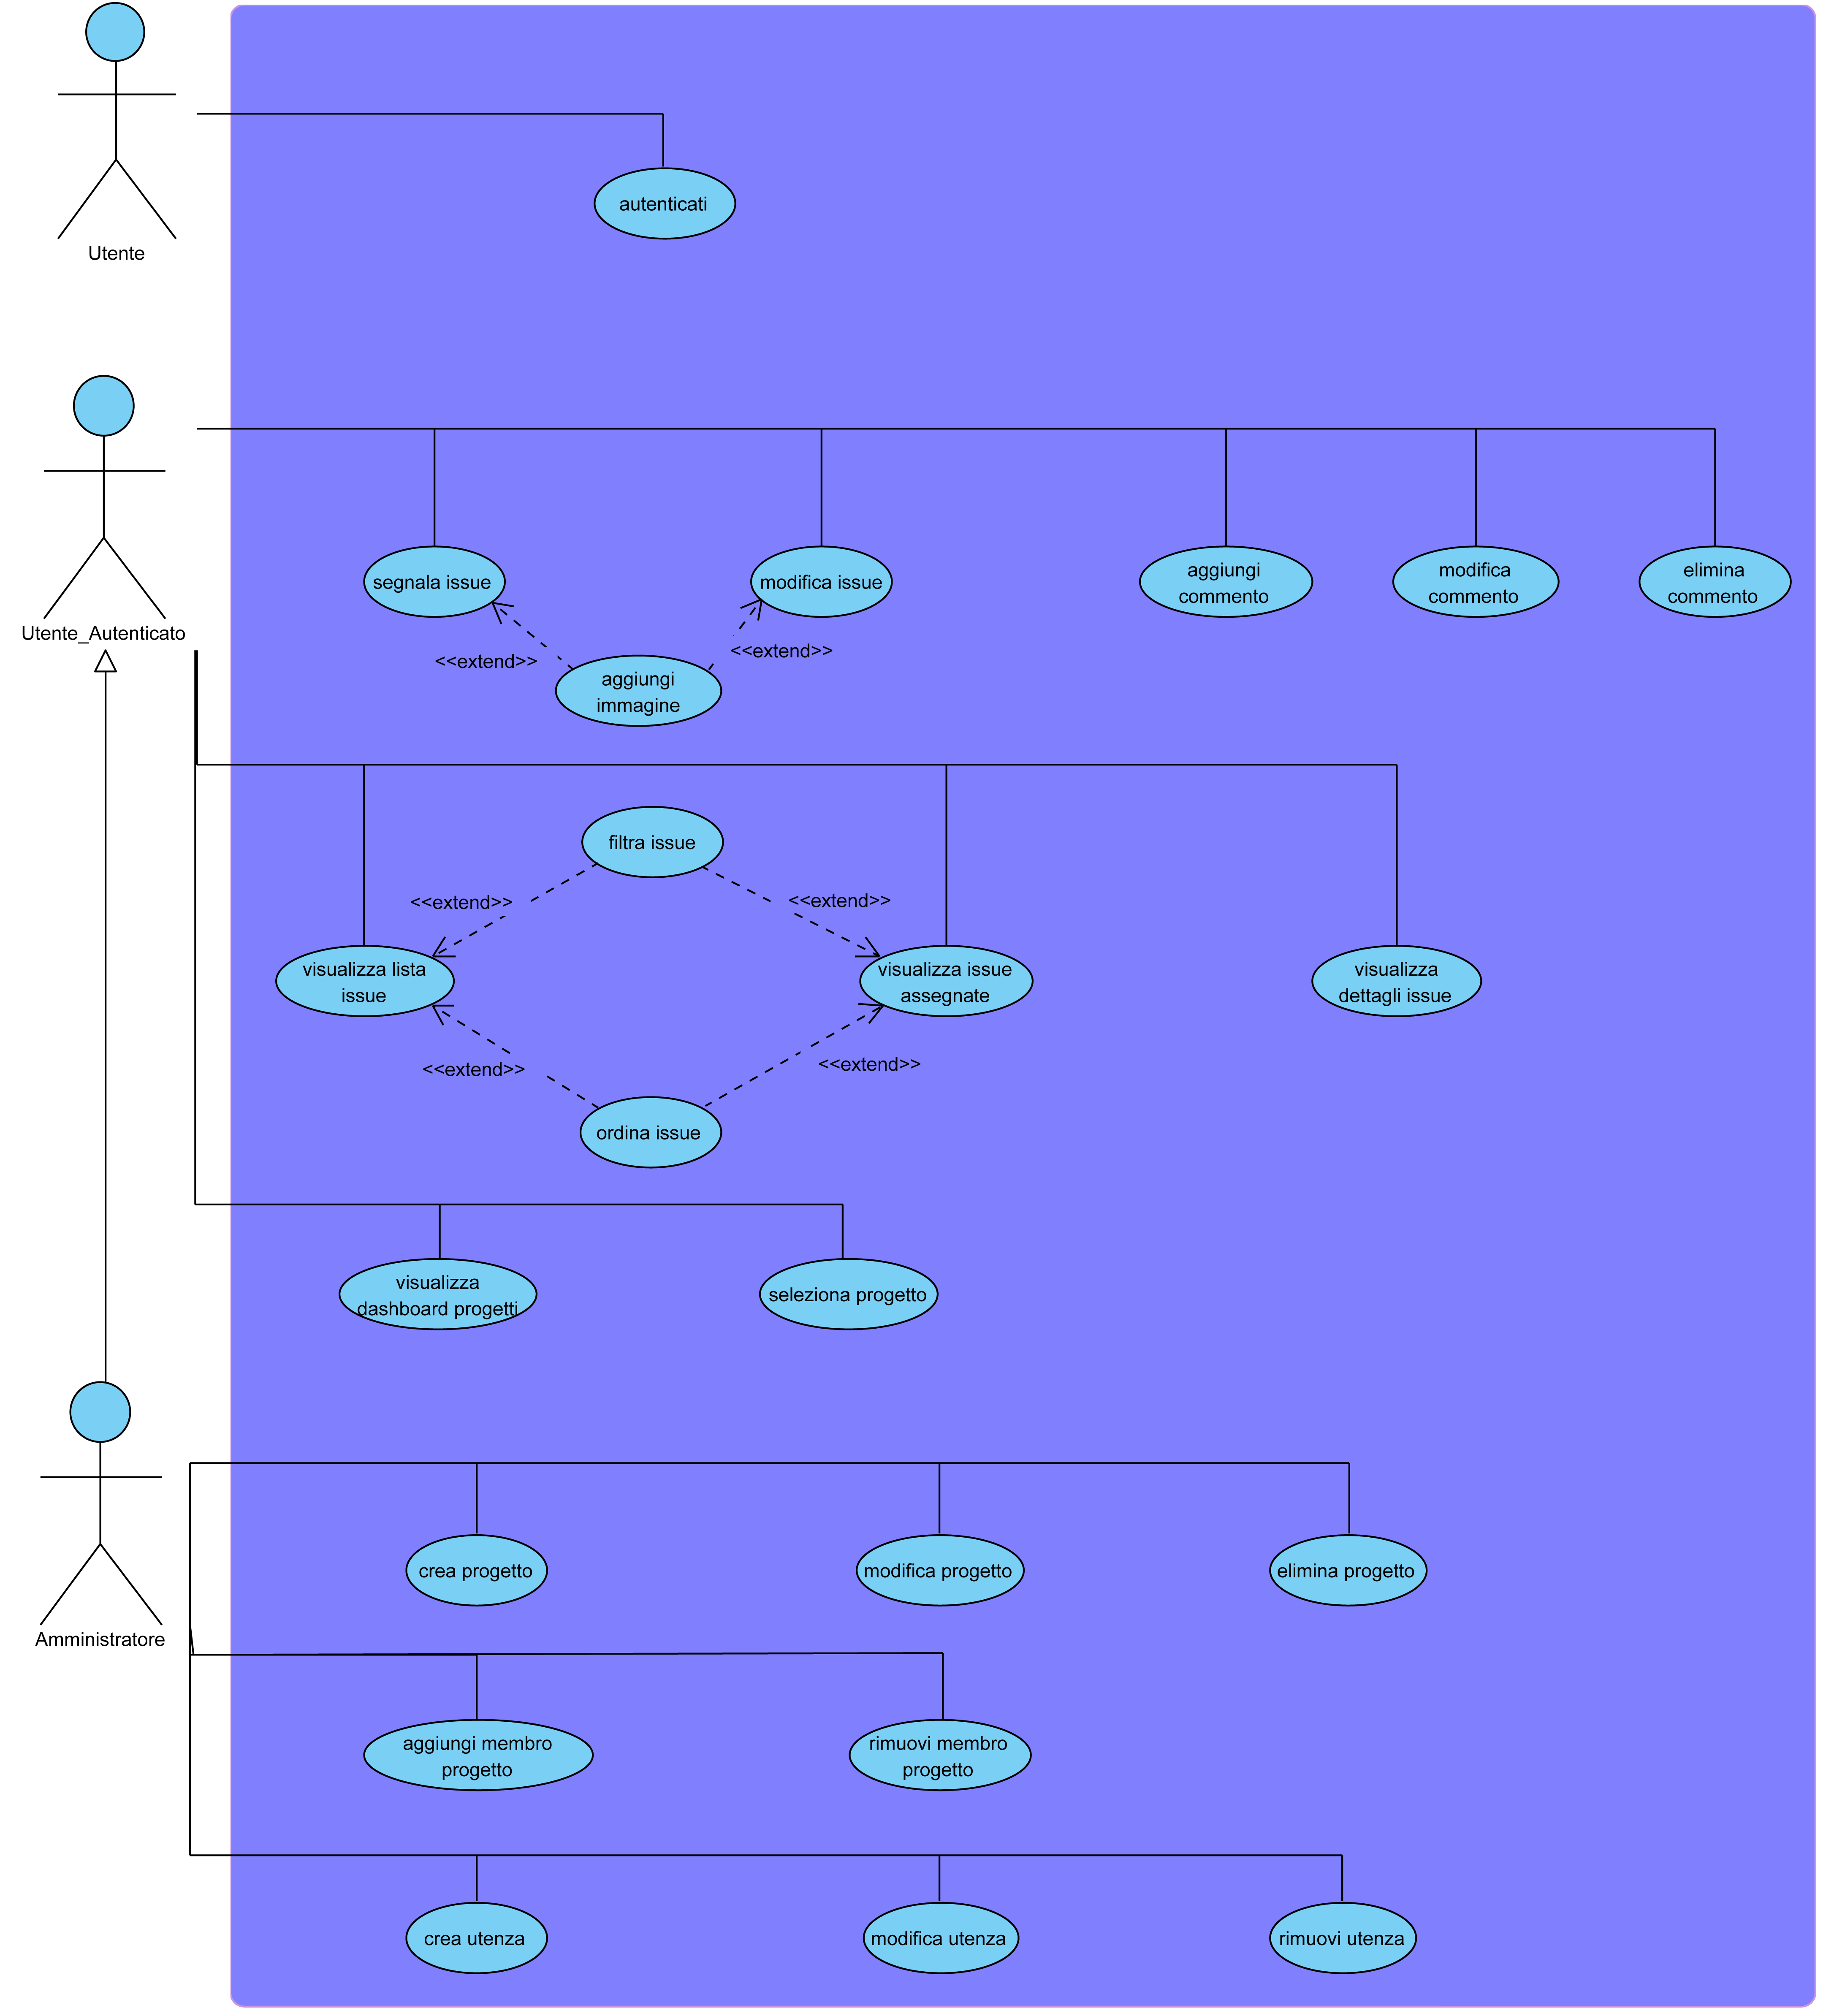
\includegraphics[width=\textwidth]{UCD1.png}
\end{figure}

\textbf{Note sul diagramma}:
\begin{itemize}[leftmargin=1.1em]
\item L'attore \textit{Utente} rappresenta qualunque individuo che accede al sistema prima dell'autenticazione.
\item L'attore \textit{Utente\_Autenticato} eredita implicitamente i permessi di \textit{Utente} e può accedere alle funzionalità di gestione issue.
\item L'attore \textit{Amministratore} eredita tutti i permessi di \textit{Utente\_Autenticato} e dispone di funzionalità privilegiate (gestione utenze, assegnazione, archiviazione, report).
\item Le relazioni \texttt{<<extend>>} indicano funzionalità opzionali che possono essere eseguite in aggiunta al caso d'uso principale.
\end{itemize}

\newpage
% ---------------------------------------------------------------------
\subsubsection{Lista dei casi d'uso}
\label{subsec:lista-use-case}
% ---------------------------------------------------------------------

Sono stati individuati i seguenti casi d'uso per il sistema \productname:

\begin{enumerate}[leftmargin=1.1em]

\item \textbf{UC-01: Autenticazione} \\
\textit{Attore primario}: Utente \\
\textit{Descrizione}: l'utente inserisce email e password per accedere al sistema.

\item \textbf{UC-02: Visualizza Dashboard Progetti} \\
\textit{Attore primario}: Utente Autenticato, Amministratore \\
\textit{Descrizione}: l'utente visualizza la lista dei progetti a cui ha accesso assegnato dall'amministratore, con statistiche e attività recenti per ciascun progetto.

\item \textbf{UC-03: Seleziona Progetto} \\
\textit{Attore primario}: Utente Autenticato, Amministratore \\
\textit{Descrizione}: l'utente seleziona uno dei progetti a cui ha accesso per visualizzarne le issue.

\item \textbf{UC-04: Crea Progetto} \\
\textit{Attore primario}: Amministratore \\
\textit{Descrizione}: l'amministratore crea un nuovo progetto specificando nome, descrizione e membri iniziali del team.

\item \textbf{UC-05: Modifica Progetto} \\
\textit{Attore primario}: Amministratore \\
\textit{Descrizione}: l'amministratore modifica nome, descrizione o altre proprietà di un progetto esistente.

\item \textbf{UC-06: Elimina Progetto} \\
\textit{Attore primario}: Amministratore \\
\textit{Descrizione}: l'amministratore elimina un progetto e tutte le sue issue associate.

\item \textbf{UC-07: Aggiungi Membri Progetto} \\
\textit{Attore primario}: Amministratore \\
\textit{Descrizione}: l'amministratore aggiunge utenti dal team di un progetto, determinando chi può accedere a quel progetto.

\item \textbf{UC-08: Rimuovi Membri Progetto} \\
\textit{Attore primario}: Amministratore \\
\textit{Descrizione}: l'amministratore rimuove utenti dal team di un progetto, determinando chi non può più accedere a quel progetto.

\item \textbf{UC-09: Segnala Issue} \\
\textit{Attore primario}: Utente Autenticato, Amministratore \\
\textit{Descrizione}: l'utente crea una nuova issue all'interno del progetto correntemente selezionato.

\item \textbf{UC-10: Visualizza Lista Issue} \\
\textit{Attore primario}: Utente Autenticato, Amministratore \\
\textit{Descrizione}: l'utente visualizza tutte le issue del progetto corrente.

\item \textbf{UC-11: Visualizza Dettagli Issue} \\
\textit{Attore primario}: Utente Autenticato, Amministratore \\
\textit{Descrizione}: l'utente visualizza il dettaglio completo di una issue del progetto corrente.

\item \textbf{UC-12: Modifica Issue} \\
\textit{Attore primario}: Utente Autenticato, Amministratore \\
\textit{Descrizione}: l'utente modifica attributi di una issue esistente nel progetto.

\item \textbf{UC-13: Aggiungi Etichette} \\
\textit{Attore primario}: Utente Autenticato, Amministratore \\
\textit{Descrizione}: l'utente associa etichette a una issue per categorizzazione.

\item \textbf{UC-14: Aggiungi Immagine} \\
\textit{Attore primario}: Utente Autenticato, Amministratore \\
\textit{Descrizione}: l'utente allega immagini a una issue.

\item \textbf{UC-15: Filtra Issue} \\
\textit{Attore primario}: Utente Autenticato, Amministratore \\
\textit{Descrizione}: l'utente applica filtri per visualizzare sottoinsiemi di issue del progetto.

\item \textbf{UC-16: Ordina Issue} \\
\textit{Attore primario}: Utente Autenticato, Amministratore \\
\textit{Descrizione}: l'utente ordina la lista issue secondo criteri specificati.

\item \textbf{UC-17: Visualizza Issue Assegnate} \\
\textit{Attore primario}: Utente Autenticato, Amministratore \\
\textit{Descrizione}: l'utente visualizza solo le issue del progetto corrente che gli sono state assegnate dall'amministratore.

\item \textbf{UC-18: Aggiungi Commento} \\
\textit{Attore primario}: Utente Autenticato, Amministratore \\
\textit{Descrizione}: l'utente aggiunge commenti testuali a una issue.

\item \textbf{UC-19: Elimina Commento} \\
\textit{Attore primario}: Utente Autenticato, Amministratore \\
\textit{Descrizione}: l'utente elimina i propri commenti.

\item \textbf{UC-20: Visualizza Notifiche} \\
\textit{Attore primario}: Utente Autenticato, Amministratore \\
\textit{Descrizione}: l'utente visualizza notifiche ricevute (assegnazioni, menzioni, aggiornamenti).

\item \textbf{UC-21: Prendi Visione Notifica} \\
\textit{Attore primario}: Utente Autenticato, Amministratore \\
\textit{Descrizione}: l'utente marca le notifiche come lette.

\item \textbf{UC-22: Creazione Utenze} \\
\textit{Attore primario}: Amministratore \\
\textit{Descrizione}: l'amministratore crea nuovi account utente.

\item \textbf{UC-23: Modifica Utenze} \\
\textit{Attore primario}: Amministratore \\
\textit{Descrizione}: l'amministratore modifica dati di account esistenti.

\item \textbf{UC-24: Rimozione Utenze} \\
\textit{Attore primario}: Amministratore \\
\textit{Descrizione}: l'amministratore elimina account utente.

\item \textbf{UC-25: Assegna Issue} \\
\textit{Attore primario}: Amministratore \\
\textit{Descrizione}: l'amministratore assegna una issue a un membro del team del progetto.

\item \textbf{UC-26: Archivia Issue} \\
\textit{Attore primario}: Amministratore \\
\textit{Descrizione}: l'amministratore archivia una issue mantenendone la tracciabilità.

\item \textbf{UC-27: Visualizza Report Mensile} \\
\textit{Attore primario}: Amministratore \\
\textit{Descrizione}: l'amministratore visualizza report mensile con metriche del progetto selezionato.

\end{enumerate}

\newpage

% ---------------------------------------------------------------------
% SEZIONE 4: CARATTERIZZAZIONE UTENTI
% ---------------------------------------------------------------------
% ---------------------------------------------------------------------
\subsection{Individuazione e caratterizzazione degli utenti del sistema}
\label{sec:caratterizzazione-utenti}
% ---------------------------------------------------------------------

Il sistema \productname{} è progettato per supportare tre distinte tipologie di utenti, ciascuna con obiettivi, responsabilità e permessi specifici. Questa sezione fornisce una caratterizzazione dettagliata di ogni profilo utente.

% ---------------------------------------------------------------------
\subsubsection{Utente}
\label{subsec:utente}
% ---------------------------------------------------------------------

\paragraph{Descrizione}
L'attore \textit{Utente} rappresenta qualunque individuo che accede all'applicazione \productname{} prima di aver completato il processo di autenticazione. Questo profilo corrisponde allo stato iniziale di interazione con il sistema, limitato alla sola schermata di login.

\paragraph{Obiettivi}
\begin{itemize}[leftmargin=1.1em]
\item Autenticarsi al sistema utilizzando credenziali valide (email e password)
\item Accedere alle funzionalità della piattaforma secondo il proprio ruolo
\end{itemize}

\paragraph{Responsabilità e permessi}
\begin{itemize}[leftmargin=1.1em]
\item \textbf{Visualizzare} la schermata di autenticazione
\item \textbf{Inserire} email e password nei campi del form di login
\item \textbf{Inviare} una richiesta di autenticazione al sistema
\item \textbf{Ricevere} messaggi di errore in caso di credenziali non valide o account bloccato
\end{itemize}

\textbf{Limitazioni}: questo profilo non ha accesso ad alcuna funzionalità operativa del sistema fino al completamento dell'autenticazione.

\newpage

% ---------------------------------------------------------------------
\subsubsection{Utente\_Autenticato}
\label{subsec:utente-autenticato}
% ---------------------------------------------------------------------

\paragraph{Descrizione}

L'\textbf{Utente Autenticato} è un membro del team che ha effettuato correttamente il login e ha accesso ai \textbf{progetti a cui è stato assegnato da un amministratore}. Questo profilo rappresenta lo sviluppatore, tester o membro del team che lavora attivamente su issue all'interno dei progetti autorizzati.

\paragraph{Obiettivi}
\begin{itemize}[leftmargin=1.1em]
\item Visualizzare i progetti a cui ha accesso assegnato dall'amministratore
\item Lavorare sulle issue dei progetti autorizzati (creazione, modifica, commenti)
\item Collaborare con il team attraverso commenti e aggiornamenti sulle issue
\item Monitorare lo stato delle issue assegnate personalmente
\item Ricevere e gestire notifiche relative ai progetti di appartenenza
\end{itemize}

\paragraph{Responsabilità e permessi}
L'Utente\_Autenticato dispone dei seguenti permessi:

\subparagraph{Gestione Progetti}
\begin{itemize}[leftmargin=1.1em]
\item \textbf{Può}: visualizzare solo i progetti a cui è stato aggiunto da un amministratore, selezionare un progetto per accedere alle sue issue
\item \textbf{Non può}: creare nuovi progetti, eliminare progetti, modificare progetti, scegliere autonomamente a quali progetti partecipare, vedere progetti di cui non è membro
\end{itemize}

\subparagraph{Gestione Issue}
\begin{itemize}[leftmargin=1.1em]
\item \textbf{Creare} nuove issue, all'interno dei progetti a cui appartiene, specificando:
  \begin{itemize}
  \item Titolo (\textit{obbligatorio})
  \item Descrizione (\textit{obbligatoria})
  \item Tipo (\textit{obbligatorio}: Bug, Feature, Question, Documentation)
  \item Priorità (\textit{opzionale}: Nessuna (Default), Bassa, Media, Alta, Critica)
  \item Etichette personalizzate (\textit{opzionale}, array di stringhe)
  \item Immagini allegate (\textit{opzionale})
  \end{itemize}
\item \textbf{Visualizzare} la lista completa delle issue del progetto selezionato
\item \textbf{Filtrare} le issue per tipo, stato, priorità, etichetta, assegnatario, intervallo di data creazione
\item \textbf{Ordinare} le issue per data di creazione, priorità, stato (crescente/decrescente)
\item \textbf{Visualizzare} il dettaglio completo di una singola issue con tutti i suoi attributi
\item \textbf{Modificare} le issue esistenti (aggiornamento di titolo, descrizione, tipo, priorità, etichette), solo per i progetti di appartenenza
\item \textbf{Associare} etichette personalizzate a una issue per facilitarne la categorizzazione
\end{itemize}

\subparagraph{Collaborazione}
\begin{itemize}[leftmargin=1.1em]
\item \textbf{Aggiungere} commenti testuali a qualunque issue
\item \textbf{Eliminare} i propri commenti
\item \textbf{Leggere} i commenti lasciati da altri utenti
\end{itemize}

\paragraph{Vista Personalizzata}
\begin{itemize}[leftmargin=1.1em]
\item \textbf{Visualizzare} una vista dedicata delle issue assegnate al proprio account
\item \textbf{Ricevere} notifiche quando una issue viene assegnata al proprio account
\item \textbf{Visualizzare} l'elenco delle notifiche ricevute
\item \textbf{Confermare} la presa visione delle notifiche
\end{itemize}

\textbf{Limitazioni}: questo profilo non può creare o modificare utenze, non può assegnare issue ad altri utenti, non può archiviare issue e non ha accesso ai report amministrativi.

\newpage

% ---------------------------------------------------------------------
\subsection{Amministratore}
\label{subsec:amministratore}
% ---------------------------------------------------------------------

\subsubsection{Descrizione}
L'\textit{Amministratore} è un utente con privilegi elevati, responsabile della gestione delle utenze, della supervisione del flusso di lavoro e del monitoraggio delle performance del team. Questo ruolo eredita completamente tutti i permessi dell'Utente\_Autenticato e dispone di funzionalità amministrative aggiuntive.

\subsubsection{Obiettivi}
\begin{itemize}[leftmargin=1.1em]
\item \textbf{Gestire} gli accessi al sistema creando, modificando e rimuovendo account utente
\item \textbf{Garantire} la presa in carico tempestiva delle issue critiche attraverso l'assegnazione esplicita ai membri del team
\item \textbf{Supervisionare} l'andamento del progetto analizzando report mensili con metriche quantitative
\item \textbf{Mantenere} ordinate le viste principali archiviando le issue non più rilevanti ma preservandone la tracciabilità
\item \textbf{Monitorare} le performance individuali e del team per supportare decisioni strategiche
\end{itemize}

\subsubsection{Responsabilità e permessi}
L'Amministratore dispone di:

\paragraph{Permessi ereditati}
\begin{itemize}[leftmargin=1.1em]
\item \textbf{Tutti} i permessi e le responsabilità dell'Utente\_Autenticato (creazione issue, visualizzazione, filtri, commenti, notifiche)
\end{itemize}

\newpage

\paragraph{Gestione Utenze}
\begin{itemize}[leftmargin=1.1em]
\item \textbf{Creare} nuove utenze specificando:
  \begin{itemize}
  \item Nome (obbligatorio)
  \item Cognome (obbligatorio)
  \item Email (obbligatoria, univoca nel sistema)
  \item Password (obbligatoria, soggetta a policy di complessità)
  \item Ruolo (obbligatorio: Utente o Amministratore)
  \end{itemize}
\item \textbf{Modificare} i dati anagrafici e le credenziali di utenze esistenti
\item \textbf{Eliminare} utenze dal sistema previa conferma con inserimento della propria password amministrativa
\end{itemize}

\paragraph{Gestione Avanzata Issue}
\begin{itemize}[leftmargin=1.1em]
\item \textbf{Assegnare} una issue a un membro specifico del team, rendendolo responsabile della sua gestione
\item \textbf{Archiviare} una issue, spostandola dalle liste principali a una sezione di archivio dedicata (la issue rimane accessibile ma non appare nelle viste standard)
\end{itemize}

\paragraph{Analisi e Reportistica}
\begin{itemize}[leftmargin=1.1em]
\item \textbf{Visualizzare} report mensili contenenti metriche aggregate sull'attività del team:
  \begin{itemize}
  \item Numero totale di issue aperte nel periodo
  \item Numero totale di issue gestite/risolte nel periodo
  \item Tempo medio di risoluzione (aggregato e per singolo utente)
  \item Distribuzione delle issue per tipo e priorità
  \item Performance individuali di ciascun membro del team
  \end{itemize}
\end{itemize}

\textbf{Nota}: il sistema è fornito con un account amministratore predefinito con credenziali di default, che permette di effettuare il primo accesso e creare ulteriori utenze.

\newpage

% ---------------------------------------------------------------------
\subsection{Riepilogo Permessi per Profilo}
\label{subsec:riepilogo-permessi}
% ---------------------------------------------------------------------

La seguente tabella riassume i permessi differenziati per ciascun profilo utente:

\begin{longtable}{|p{0.35\linewidth}|c|c|c|}
\hline
\textbf{Funzionalità} & \textbf{Utente} & \textbf{Utente Aut.} & \textbf{Admin} \\ \hline
\endfirsthead

\hline
\textbf{Funzionalità} & \textbf{Utente} & \textbf{Utente Aut.} & \textbf{Admin} \\ \hline
\endhead

\hline
\endfoot

Autenticazione (login) & \cmark & \cmark & \cmark \\ \hline
Visualizza dashboard progetti & \xmark & \cmark (solo assegnati) & \cmark (tutti) \\ \hline
Crea progetto & \xmark & \xmark & \cmark \\ \hline
Modifica progetto & \xmark & \xmark & \cmark \\ \hline
Elimina progetto & \xmark & \xmark & \cmark \\ \hline
Gestisci membri progetto & \xmark & \xmark & \cmark \\ \hline
Seleziona progetto & \xmark & \cmark (solo assegnati) & \cmark (tutti) \\ \hline
Crea issue & \xmark & \cmark (progetti autorizzati) & \cmark \\ \hline
Visualizza issue & \xmark & \cmark (progetti autorizzati) & \cmark (tutti) \\ \hline
Modifica issue & \xmark & \cmark (progetti autorizzati) & \cmark (tutti) \\ \hline
Assegna issue & \xmark & \xmark & \cmark \\ \hline
Archivia issue & \xmark & \xmark & \cmark \\ \hline
Aggiungi commento & \xmark & \cmark & \cmark \\ \hline
Elimina proprio commento & \xmark & \cmark & \cmark \\ \hline
Filtra/ordina issue & \xmark & \cmark & \cmark \\ \hline
Aggiungi etichette/immagini & \xmark & \cmark & \cmark \\ \hline
Visualizza notifiche & \xmark & \cmark & \cmark \\ \hline
Crea utenza & \xmark & \xmark & \cmark \\ \hline
Modifica utenza & \xmark & \xmark & \cmark \\ \hline
Elimina utenza & \xmark & \xmark & \cmark \\ \hline
Visualizza report & \xmark & \xmark & \cmark \\ \hline

\end{longtable}

\textbf{Legenda}:
\begin{itemize}[leftmargin=1.1em]
\item \cmark{} = Permesso concesso
\item \xmark{} = Permesso negato
\item "solo assegnati" = può accedere solo a progetti in cui appare in \texttt{Project\_Member}
\item "progetti autorizzati" = operazioni limitate ai progetti di appartenenza
\end{itemize}

\newpage

% ---------------------------------------------------------------------
% SEZIONE 5: REQUISITI SPECIFICI
% ---------------------------------------------------------------------
\subsection{Requisiti Specifici}
\label{sec:requisiti-specifici}

% ---------------------------------------------------------------------
\subsubsection{Requisiti di Sistema}
\label{subsec:requisiti-sistema}
% ---------------------------------------------------------------------

Questa sezione dettaglia i requisiti specifici che il sistema \productname{} deve soddisfare. 
I requisiti sono definiti da una prospettiva esterna, descrivendo le interazioni del sistema con i suoi utenti e con altri sistemi.

% ---------------------------------------------------------------------
\paragraph{Requisiti delle Interfacce Esterne}
\label{subsubsec:interfacce-esterne}
% ---------------------------------------------------------------------

\subparagraph{Interfaccia Utente (User Interface)}
Il sistema dovrà fornire un'interfaccia utente grafica (GUI) web-based, accessibile tramite i browser moderni. 
L'interfaccia dovrà essere responsive, garantendo l'usabilità su schermi di diverse dimensioni, dai dispositivi mobili
(minimo 320px di larghezza) ai desktop. 
Tutte le funzionalità esposte agli utenti dovranno essere accessibili tramite tale interfaccia.

\subparagraph{Interfaccia Software (Software Interface)}
Il sistema dovrà esporre un'interfaccia di programmazione (API) basata sullo stile architetturale REST 
per consentire la comunicazione tra il componente front-end e il back-end. 
Queste API dovranno utilizzare il formato JSON per lo scambio di dati e seguire 
le convenzioni standard del protocollo HTTP per le operazioni (GET, POST, PUT, DELETE). 
Questo garantirà l'interoperabilità e la possibilità di sviluppare client alternativi in futuro.

\subparagraph{Interfaccia di Comunicazione (Communications Interface)}
Tutta la comunicazione tra il client e il server che trasporta dati sensibili 
(incluse le credenziali di autenticazione e i dati delle issue) 
dovrà avvenire tramite protocolli di comunicazione sicuri (HTTPS).

% ---------------------------------------------------------------------
\paragraph{Requisiti Prestazionali}
\label{subsubsec:requisiti-prestazionali}
% ---------------------------------------------------------------------
Il sistema dovrà rispettare i requisiti di performance specificati nella sezione dei 
Requisiti Non Funzionali (REQ-NFR-01), garantendo tempi di risposta rapidi per le operazioni interattive.

% ---------------------------------------------------------------------
\paragraph{Requisiti del Database Logico}
\label{subsubsec:database-logico}
% ---------------------------------------------------------------------
Il sistema dovrà garantire la persistenza, la consistenza e l'integrità dei dati. 
Dovrà gestire le seguenti entità logiche principali e le loro relazioni: 
Utenti, Progetti, Issue, Commenti, Etichette, Allegati e le associazioni tra di esse 
(es. Utenti membri di Progetti, Issue appartenenti a Progetti). 
Il sistema dovrà garantire che le operazioni sul database siano transazionali per prevenire la corruzione dei dati in caso di fallimenti.
\newpage
% ---------------------------------------------------------------------
\subsubsection{Requisiti Funzionali}
\label{subsec:requisiti-funzionali}
% ---------------------------------------------------------------------

Questa sottosezione descrive in dettaglio tutte le funzionalità del sistema \productname, specificando input, elaborazione e output secondo lo standard IEEE 830-1998. Il sistema è organizzato gerarchicamente: gli \textbf{Amministratori} creano \textbf{Progetti} e assegnano \textbf{Utenti} ad essi; all'interno di ogni progetto, i membri autorizzati gestiscono \textbf{Issue}.

\vspace{0.5cm}

% =====================================================================
% REQ-FUN-01
% =====================================================================

\begin{reqbox}[title=REQ-FUN-01: Autenticazione]
\label{subsubsec:req-autenticazione}

\subparagraph{Introduzione}
Il sistema deve fornire un meccanismo di autenticazione sicuro per accesso alla piattaforma.

\subparagraph{Input}
\begin{itemize}[leftmargin=1.1em]
\item Email (obbligatorio, formato valido)
\item Password (obbligatorio, min 8 caratteri)
\end{itemize}

\subparagraph{Elaborazione}
\begin{enumerate}[leftmargin=1.1em]
\item Valida formato email e presenza campi
\item Cerca account nel database
\item Se valida: crea sessione
\item Se non valida: incrementa contatore tentativi
\end{enumerate}

\subparagraph{Output}
\textbf{Successo}: Reindirizzamento a dashboard progetti

\textbf{Errore}: "Credenziali non valide", "Account bloccato", "Campi obbligatori"

\end{reqbox}

\vspace{0.5cm}

\newpage

% =====================================================================
% REQ-FUN-02
% =====================================================================

\begin{reqbox}[title=REQ-FUN-02: Visualizza Dashboard Progetti]
\label{subsubsec:req-dashboard-progetti}

\subparagraph{Introduzione}
Dopo l'autenticazione, l'utente visualizza la dashboard con i \textbf{progetti a cui ha accesso} assegnati dall'amministratore.

\subparagraph{Precondizioni}
Utente autenticato.

\subparagraph{Input}
Caricamento automatico post-login.

\subparagraph{Elaborazione}
\begin{enumerate}[leftmargin=1.1em]
\item Recupera l'utente autenticato dal database
\item Recupera i progetti legati all'utente
\end{enumerate}

\subparagraph{Output}
Dashboard con:
\begin{itemize}[leftmargin=1.1em]
\item Card progetti: nome, descrizione, statistiche
\item Pulsante "Accedi" per selezionare un progetto
\item Se nessun progetto: "Nessun progetto disponibile."
\item Se admin: pulsante "+ Crea Nuovo Progetto"
\end{itemize}

\end{reqbox}

\vspace{0.5cm}

\newpage

% =====================================================================
% REQ-FUN-03
% =====================================================================

\begin{reqbox}[title=REQ-FUN-03: Seleziona Progetto]
\label{subsubsec:req-seleziona-progetto}

\paragraph{Introduzione}
L'utente seleziona un progetto per accedere alle sue issue.

\paragraph{Precondizioni}
Utente autenticato con almeno un progetto assegnato.

\paragraph{Input}
Click su progetto dalla dashboard.

\paragraph{Elaborazione}
\begin{enumerate}[leftmargin=1.1em]
\item Verifica che l'utente appartenga al progetto selezionato
\item Imposta il progetto corrente nella sessione
\item Recupera le issue del progetto
\item Reindirizza alla lista issue
\end{enumerate}

\paragraph{Output}
\textbf{Successo}: Entra nel contesto del progetto, header mostra nome progetto, visualizza lista issue

\textbf{Errore}: "Accesso negato. Non fai parte di questo progetto."

\end{reqbox}

\vspace{0.5cm}

\newpage

% =====================================================================
% REQ-FUN-04
% =====================================================================

\begin{reqbox}[title=REQ-FUN-04: Crea Progetto (solo Admin)]
\label{subsubsec:req-crea-progetto}

\paragraph{Introduzione}
Solo gli amministratori possono creare nuovi progetti.

\paragraph{Precondizioni}
Utente con ruolo Amministratore.

\paragraph{Input}
\begin{itemize}[leftmargin=1.1em]
\item Nome progetto (obbligatorio, univoco)
\item Descrizione (opzionale)
\item Membri iniziali (obbligatorio, multi-selezione utenti, con almeno un membro)
\end{itemize}

\paragraph{Elaborazione}
\begin{enumerate}[leftmargin=1.1em]
\item Verifica ruolo amministratore
\item Valida unicità nome progetto
\item Crea nuovo progetto nel database
\item Associa i membri selezionati al progetto
\item Aggiunge automaticamente l'amministratore creatore come membro
\end{enumerate}

\paragraph{Output}
\textbf{Successo}: "Progetto '[Nome]' creato con successo"

\textbf{Errore}: "Nome già esistente", "Permessi insufficienti"

\end{reqbox}

\vspace{0.5cm}

\newpage

% =====================================================================
% REQ-FUN-05
% =====================================================================

\begin{reqbox}[title=REQ-FUN-05: Modifica Progetto (solo Admin)]
\label{subsubsec:req-modifica-progetto}

\paragraph{Introduzione}
Gli amministratori possono modificare nome e descrizione di progetti esistenti.

\paragraph{Precondizioni}
Amministratore, progetto esistente.

\paragraph{Input}
Nuovo nome (se modificato deve essere univoco), nuova descrizione.

\paragraph{Elaborazione}
\begin{enumerate}[leftmargin=1.1em]
\item Verifica ruolo amministratore
\item Se nome modificato: verifica unicità
\item Aggiorna i dati del progetto nel database
\end{enumerate}

\paragraph{Output}
\textbf{Successo}: "Progetto aggiornato con successo"

\textbf{Errore}: "Nome già in uso", "Permessi insufficienti"

\end{reqbox}

\vspace{0.5cm}

\newpage

% =====================================================================
% REQ-FUN-06
% =====================================================================

\begin{reqbox}[title=REQ-FUN-06: Elimina Progetto (solo Admin)]
\label{subsubsec:req-elimina-progetto}

\paragraph{Introduzione}
Gli amministratori possono eliminare progetti con tutte le issue associate.

\paragraph{Precondizioni}
Amministratore, progetto esistente.

\paragraph{Input}
Selezione progetto, conferma con password amministratore.

\paragraph{Elaborazione}
\begin{enumerate}[leftmargin=1.1em]
\item Mostra dialog conferma: "Eliminare progetto? Tutte le issue saranno eliminate. Operazione irreversibile."
\item Verifica password amministratore
\item Elimina tutte le issue, commenti, etichette e allegati del progetto
\item Rimuove associazioni membri-progetto
\item Elimina il progetto dal database
\end{enumerate}

\paragraph{Output}
\textbf{Successo}: "Progetto '[Nome]' e tutte le sue issue eliminate"

\textbf{Errore}: "Password non valida"

\end{reqbox}

\vspace{0.5cm}

\newpage

% =====================================================================
% REQ-FUN-07
% =====================================================================

\begin{reqbox}[title=REQ-FUN-07: Aggiungi Membri Progetto (solo Admin)]
\label{subsubsec:req-gestisci-membri}

\paragraph{Introduzione}
Gli amministratori decidono quali utenti possono accedere a ciascun progetto.

\paragraph{Precondizioni}
Amministratore, progetto esistente.

\paragraph{Input}
Selezione utenti da aggiungere al progetto.

\paragraph{Elaborazione}

\textbf{Aggiunta membro}:
\begin{enumerate}[leftmargin=1.1em]
\item Verifica che l'utente non sia già membro del progetto
\item Associa l'utente al progetto nel database
\item Notifica l'utente dell'aggiunta
\end{enumerate}

\paragraph{Output}
\textbf{Successo}: "Utente [Nome] aggiunto al progetto"

\textbf{Errore}: "Utente già membro".

\end{reqbox}

\vspace{0.5cm}

\newpage

% =====================================================================
% REQ-FUN-08
% =====================================================================

\begin{reqbox}[title=REQ-FUN-08: Rimuovi Membri Progetto (solo Admin)]
\label{subsubsec:req-gestisci-membri}

\paragraph{Introduzione}
Gli amministratori decidono quali utenti devono essere rimossi da un determinato progetto.

\paragraph{Precondizioni}
Amministratore, progetto esistente, utente\_autenticato membro del progetto

\paragraph{Input}
Selezione utenti da rimuovere dal progetto.

\paragraph{Elaborazione}

\textbf{Rimozione membro}:
\begin{enumerate}[leftmargin=1.1em]
\item Verifica che il progetto abbia almeno un altro membro
\item Rimuove le assegnazioni issue dell'utente nel progetto
\item Rimuove l'associazione utente-progetto dal database
\item Notifica l'utente della rimozione
\end{enumerate}

\paragraph{Output}
\textbf{Successo}: "Utente [Nome] rimosso dal progetto"

\textbf{Errore}: "Impossibile rimuovere ultimo membro"

\end{reqbox}

\vspace{0.5cm}

\newpage

% =====================================================================
% REQ-FUN-09
% =====================================================================

\begin{reqbox}[title=REQ-FUN-09: Segnala Issue]
\label{subsubsec:req-segnala-issue}

\paragraph{Introduzione}
Gli utenti creano nuove issue all'interno del \textbf{progetto correntemente selezionato}.

\paragraph{Precondizioni}
Utente autenticato, progetto selezionato, utente membro del progetto.

\paragraph{Input}
\begin{itemize}[leftmargin=1.1em]
\item Titolo (obbligatorio)
\item Descrizione (obbligatoria)
\item Tipo (obbligatorio: Bug, Feature, Question, Documentation)
\item Priorità (opzionale: Nessuna, Bassa, Media, Alta, Critica)
\item Etichette (opzionale)
\item Immagini (opzionale)
\end{itemize}

\paragraph{Elaborazione}
\begin{enumerate}[leftmargin=1.1em]
\item Verifica che l'utente appartenga al progetto corrente
\item Valida tutti i campi obbligatori e i vincoli di formato
\item Se presenti immagini: carica i file su storage
\item Se priorità non specificata: imposta a "Nessuna"
\item Crea la nuova issue associata al progetto corrente con stato "ToDo"
\item Se priorità è "Critica": notifica gli amministratori del progetto
\end{enumerate}

\paragraph{Output}
\textbf{Successo}: "Issue \#[ID] creata con successo", reindirizzamento a dettaglio issue

\textbf{Errore}: "Campo obbligatorio mancante", "Immagine troppo grande", "Formato non supportato"

\end{reqbox}

\vspace{0.5cm}

\newpage

% =====================================================================
% REQ-FUN-10
% =====================================================================

\begin{reqbox}[title=REQ-FUN-10: Visualizza Lista Issue]
\label{subsubsec:req-visualizza-lista-issue}

\paragraph{Introduzione}
Gli utenti visualizzano tutte le issue del \textbf{progetto corrente}.

\paragraph{Precondizioni}
Utente autenticato, progetto selezionato, membro del progetto.

\paragraph{Input}
Accesso a sezione "Issue" o automatico dopo selezione progetto.

\paragraph{Elaborazione}
\begin{enumerate}[leftmargin=1.1em]
\item Verifica appartenenza al progetto corrente
\item Recupera tutte le issue del progetto non archiviate
\item Per ogni issue recupera: ID, titolo, tipo, priorità, stato, autore, assegnatario, data
\item Applica eventuali filtri e ordinamenti salvati in sessione
\end{enumerate}

\paragraph{Output}
Lista issue con: tabella o card, icona tipo, titolo cliccabile, priorità (badge colorato), stato, assegnatario, pulsante "Crea Nuova Issue".

\end{reqbox}

\vspace{0.5cm}

\newpage

% =====================================================================
% REQ-FUN-11
% =====================================================================

\begin{reqbox}[title=REQ-FUN-11: Visualizza Dettagli Issue]
\label{subsubsec:req-visualizza-dettagli-issue}

\paragraph{Introduzione}
Gli utenti visualizzano il dettaglio completo di una issue del progetto corrente.

\paragraph{Precondizioni}
Utente autenticato, membro del progetto della issue.

\paragraph{Input}
Click su issue dalla lista.

\paragraph{Elaborazione}
\begin{enumerate}[leftmargin=1.1em]
\item Verifica che la issue appartenga al progetto corrente
\item Verifica che l'utente sia membro del progetto
\item Recupera tutti i dettagli della issue: informazioni base, commenti, etichette, immagini
\end{enumerate}

\paragraph{Output}
Pagina dettaglio / Modale con: header (ID, titolo, tipo, priorità, stato), informazioni (autore, data creazione, assegnatario), descrizione formattata, etichette, immagini (galleria), sezione commenti, pulsanti "Modifica" e "Archivia" (se amministratore).

\textbf{Errore}: "Issue non trovata" o "Accesso negato" se progetto non autorizzato.

\end{reqbox}

\vspace{0.5cm}

\newpage

% =====================================================================
% REQ-FUN-12
% =====================================================================

\begin{reqbox}[title=REQ-FUN-12: Modifica Issue]
\label{subsubsec:req-modifica-issue}

\paragraph{Introduzione}
Gli utenti possono modificare gli attributi delle issue del progetto corrente.

\paragraph{Precondizioni}
Utente autenticato, membro del progetto, issue non archiviata.

\paragraph{Input}
Modifiche a: titolo, descrizione, tipo, priorità, stato, etichette.

\paragraph{Elaborazione}
\begin{enumerate}[leftmargin=1.1em]
\item Verifica appartenenza al progetto
\item Valida tutti i campi modificati
\item Confronta i valori con quelli precedenti
\item Aggiorna la issue nel database
\item Se priorità diventa "Critica": notifica amministratori
\item Se stato diventa "Risolta": notifica autore della issue
\end{enumerate}

\paragraph{Output}
\textbf{Successo}: "Issue aggiornata con successo"

\end{reqbox}

\vspace{0.5cm}

\newpage

% =====================================================================
% REQ-FUN-13
% =====================================================================

\begin{reqbox}[title=REQ-FUN-13: Aggiungi Etichette]
\label{subsubsec:req-aggiungi-etichette}

\paragraph{Introduzione}
Gli utenti possono associare etichette personalizzate alle issue per facilitarne la categorizzazione.

\paragraph{Precondizioni}
Utente autenticato, membro del progetto.

\paragraph{Input}
Testo etichetta.

\paragraph{Elaborazione}
\begin{enumerate}[leftmargin=1.1em]
\item Normalizza il testo dell'etichetta
\item Verifica che non sia già associata alla issue
\item Verifica che il totale etichette non superi 10
\item Associa l'etichetta alla issue
\end{enumerate}

\paragraph{Output}
\textbf{Aggiunta}: Tag colorato visibile immediatamente.

\textbf{Rimozione}: Click su X del tag rimuove l'etichetta dalla issue.

\end{reqbox}

\vspace{0.5cm}

\newpage

% =====================================================================
% REQ-FUN-14
% =====================================================================

\begin{reqbox}[title=REQ-FUN-14: Aggiungi Immagine]
\label{subsubsec:req-aggiungi-immagine}

\paragraph{Introduzione}
Gli utenti possono allegare immagini alle issue per fornire documentazione visuale.

\paragraph{Input}
File immagine PNG o JPG.

\paragraph{Elaborazione}
\begin{enumerate}[leftmargin=1.1em]
\item Valida formato file e dimensione
\item Genera nome file univoco
\item Carica il file su storage
\item Associa l'immagine alla issue nel database
\end{enumerate}

\paragraph{Output}
\textbf{Successo: } "Immagine caricata con successo", pulsante "Rimuovi".

\textbf{Errore}: "Formato non supportato. Usa PNG o JPG"

\end{reqbox}

\vspace{0.5cm}

\newpage

% =====================================================================
% REQ-FUN-15
% =====================================================================

\begin{reqbox}[title=REQ-FUN-15: Filtra Issue]
\label{subsubsec:req-filtra-issue}

\paragraph{Introduzione}
Gli utenti possono applicare filtri per visualizzare sottoinsiemi specifici di issue del \textbf{progetto corrente}.

\paragraph{Input}
Selezione criteri di filtro: Tipo, Stato, Priorità, Etichetta, Assegnatario, Autore, Data creazione (range).

\paragraph{Elaborazione}
\begin{enumerate}[leftmargin=1.1em]
\item Costruisce i criteri di filtro selezionati dall'utente
\item Recupera dal database solo le issue del progetto corrente che soddisfano tutti i criteri
\item Salva i filtri applicati nella sessione per persistenza
\end{enumerate}

\paragraph{Output}
Lista issue aggiornata con solo gli elementi filtrati, badge "X filtri attivi".

\end{reqbox}

\vspace{0.5cm}

\newpage

% =====================================================================
% REQ-FUN-16
% =====================================================================

\begin{reqbox}[title=REQ-FUN-16: Ordina Issue]
\label{subsubsec:req-ordina-issue}

\paragraph{Introduzione}
Gli utenti possono ordinare la lista issue secondo criteri specificati.

\paragraph{Input}
Campo di ordinamento (Data creazione, Priorità, Stato, Titolo) e direzione (Crescente o Decrescente).

\paragraph{Elaborazione}
\begin{enumerate}[leftmargin=1.1em]
\item Applica l'ordinamento richiesto alla lista issue
\item Per Priorità usa ordine: Critica, Alta, Media, Bassa
\item Per Stato usa ordine: ToDo, In Lavorazione, In Revisione, Risolta, Chiusa
\item Salva la preferenza di ordinamento nella sessione
\end{enumerate}

\paragraph{Output}
Lista issue riordinata secondo il criterio selezionato, indicatore visuale (freccia) sulla colonna ordinata, persistenza durante la navigazione.

\end{reqbox}

\vspace{0.5cm}

\newpage

% =====================================================================
% REQ-FUN-17
% =====================================================================

\begin{reqbox}[title=REQ-FUN-17: Visualizza Issue Assegnate]
\label{subsubsec:req-visualizza-issue-assegnate}

\paragraph{Introduzione}
Gli utenti visualizzano una vista dedicata con solo le issue del \textbf{progetto corrente} assegnate a loro.

\paragraph{Input}
Click su "Le Mie Issue" dal menu.

\paragraph{Elaborazione}
\begin{enumerate}[leftmargin=1.1em]
\item Recupera tutte le issue del progetto corrente assegnate all'utente
\item Esclude le issue archiviate
\end{enumerate}

\paragraph{Output}
Lista filtrata con solo le issue assegnate all'utente, organizzazione per stato (ToDo, In Lavorazione, In Revisione, Risolta, Chiusa), possibilità di cambiare stato direttamente.

\end{reqbox}

\vspace{0.5cm}

\newpage

% =====================================================================
% REQ-FUN-18
% =====================================================================

\begin{reqbox}[title=REQ-FUN-18: Aggiungi Commento]
\label{subsubsec:req-aggiungi-commento}

\paragraph{Introduzione}
Gli utenti possono aggiungere commenti testuali alle issue per discussione e collaborazione.

\paragraph{Input}
Testo commento (obbligatorio).

\paragraph{Elaborazione}
\begin{enumerate}[leftmargin=1.1em]
\item Valida lunghezza testo
\item Sanitizza l'input
\item Crea nuovo commento associato alla issue con timestamp e autore
\item Se il commento menziona altri utenti (@username): invia notifiche
\item Aggiorna timestamp ultima modifica della issue
\end{enumerate}

\paragraph{Output}
Commento appare immediatamente nella sezione commenti con avatar autore, nome, timestamp, testo formattato, pulsante "Elimina" (visibile solo all'autore), toast "Commento aggiunto"

\end{reqbox}

\vspace{0.5cm}

\newpage

% =====================================================================
% REQ-FUN-19
% =====================================================================

\begin{reqbox}[title=REQ-FUN-19: Elimina Commento]
\label{subsubsec:req-elimina-commento}

\paragraph{Introduzione}
Gli utenti possono eliminare i propri commenti; gli amministratori possono eliminare qualsiasi commento.

\paragraph{Precondizioni}
Autore del commento oppure amministratore.

\paragraph{Elaborazione}
\begin{enumerate}[leftmargin=1.1em]
\item Mostra dialog conferma: "Eliminare commento? Operazione irreversibile."
\item Se confermato: elimina il commento dal database o lo marca come eliminato
\end{enumerate}

\paragraph{Output}
Commento scompare dalla lista o mostra "[Commento eliminato]", toast "Commento eliminato"

\end{reqbox}

\vspace{0.5cm}

\newpage

% =====================================================================
% REQ-FUN-19
% =====================================================================

\begin{reqbox}[title=REQ-FUN-19: Visualizza Notifiche]
\label{subsubsec:req-visualizza-notifiche}

\paragraph{Introduzione}
Gli utenti visualizzano notifiche relative ai progetti a cui hanno accesso.

\paragraph{Input}
Click sull'icona campanella nell'header.

\paragraph{Elaborazione}
\begin{enumerate}[leftmargin=1.1em]
\item Recupera tutte le notifiche dell'utente
\item Filtra per progetti a cui l'utente ha accesso
\item Ordina per timestamp decrescente (più recenti in alto)
\item Separa notifiche lette da non lette
\end{enumerate}

\paragraph{Output}
Dropdown o pagina notifiche con: lista notifiche (icona tipo, testo, timestamp relativo "2 ore fa"), badge rosso con numero notifiche non lette, evidenziazione notifiche non lette, pulsante "Segna tutte come lette"

\textbf{Tipi notifiche}: Issue assegnata, Issue Critica creata (solo admin), Issue risolta (per autore), Menzione in commento, Nuovo commento su issue seguita.

\end{reqbox}

\vspace{0.5cm}

\newpage

% =====================================================================
% REQ-FUN-20
% =====================================================================

\begin{reqbox}[title=REQ-FUN-20: Prendi Visione Notifica]
\label{subsubsec:req-prendi-visione-notifica}

\paragraph{Introduzione}
Gli utenti possono marcare le notifiche come lette.

\paragraph{Elaborazione}
\begin{enumerate}[leftmargin=1.1em]
\item Marca la notifica come letta nel database
\item Aggiunge timestamp di lettura
\item Decrementa il contatore badge notifiche non lette
\end{enumerate}

\paragraph{Output}
Notifica cambia aspetto (sfondo normale invece di evidenziato), badge contatore aggiornato, se cliccata reindirizza alla issue o commento relativo.

\end{reqbox}

\vspace{0.5cm}

\newpage

% =====================================================================
% REQ-FUN-21
% =====================================================================

\begin{reqbox}[title=REQ-FUN-21: Creazione Utenze (solo Admin)]
\label{subsubsec:req-creazione-utenze}

\paragraph{Introduzione}
Gli amministratori possono creare nuovi account utente.

\paragraph{Input}
Nome, Cognome, Email (univoca), Password (min 8 caratteri con requisiti di complessità), Ruolo (Utente o Amministratore).

\paragraph{Elaborazione}
\begin{enumerate}[leftmargin=1.1em]
\item Verifica ruolo amministratore
\item Valida tutti i campi e unicità email
\item Valida complessità password (almeno 1 maiuscola, 1 minuscola, 1 numero, 1 carattere speciale)
\item Crea nuovo account utente nel database
\end{enumerate}

\paragraph{Output}
\textbf{Successo}: "Utente [Nome Cognome] creato con successo", reindirizzamento a lista utenti

\textbf{Errore}: "Email già registrata", "Password non rispetta requisiti di complessità"

\end{reqbox}

\vspace{0.5cm}

\newpage

% =====================================================================
% REQ-FUN-22
% =====================================================================

\begin{reqbox}[title=REQ-FUN-22: Modifica Utenze (solo Admin)]
\label{subsubsec:req-modifica-utenze}

\paragraph{Introduzione}
Gli amministratori possono modificare i dati degli account esistenti.

\paragraph{Input}
Selezione utente, modifiche a: Nome, Cognome, Email, Password (opzionale), Ruolo.

\paragraph{Elaborazione}
\begin{enumerate}[leftmargin=1.1em]
\item Verifica che l'utente da modificare esista
\item Previene auto-modifica del ruolo amministratore corrente
\item Se email modificata: verifica unicità
\item Se password modificata: genera nuovo hash e invalida sessioni attive dell'utente
\item Aggiorna i dati dell'account nel database
\end{enumerate}

\paragraph{Output}
\textbf{Successo}: "Utente aggiornato con successo"

\textbf{Errore}: "Email già in uso", "Non puoi modificare il tuo ruolo amministratore"

\end{reqbox}

\vspace{0.5cm}

\newpage

% =====================================================================
% REQ-FUN-23
% =====================================================================

\begin{reqbox}[title=REQ-FUN-23: Rimozione Utenze (solo Admin)]
\label{subsubsec:req-rimozione-utenze}

\paragraph{Introduzione}
Gli amministratori possono eliminare account utente previa conferma.

\paragraph{Input}
Selezione utente da eliminare, password amministratore per conferma.

\paragraph{Elaborazione}
\begin{enumerate}[leftmargin=1.1em]
\item Dialog: "Eliminare utente? Operazione irreversibile. Le issue create rimarranno ma l'autore sarà marcato come 'eliminato'."
\item Verifica password amministratore
\item Previene auto-eliminazione
\item Invalida tutte le sessioni attive dell'utente
\item Marca le issue create dall'utente come "autore eliminato"
\item Rimuove l'utente da tutte le assegnazioni issue
\item Rimuove l'utente da tutti i progetti
\item Elimina l'account dal database
\end{enumerate}

\paragraph{Output}
\textbf{Successo}: "Utente [Nome Cognome] eliminato"

\textbf{Errore}: "Password amministratore non valida", "Non puoi eliminare il tuo account"

\end{reqbox}

\vspace{0.5cm}

\newpage

% =====================================================================
% REQ-FUN-24
% =====================================================================

\begin{reqbox}[title=REQ-FUN-24: Assegna Issue (solo Admin)]
\label{subsubsec:req-assegna-issue}

\paragraph{Introduzione}
Gli amministratori possono assegnare issue a membri del team del progetto.

\paragraph{Precondizioni}
Amministratore, issue e utente target esistenti, utente target membro del progetto della issue.

\paragraph{Input}
Issue da assegnare, selezione utente assegnatario dalla lista membri del progetto.

\paragraph{Elaborazione}
\begin{enumerate}[leftmargin=1.1em]
\item Verifica che l'utente target sia membro del progetto
\item Aggiorna l'assegnatario della issue
\item Se la issue era già assegnata: notifica il precedente assegnatario della riassegnazione
\item Crea notifica per il nuovo assegnatario
\end{enumerate}

\paragraph{Output}
"Issue \#[ID] assegnata a [Nome]", issue appare in "Le Mie Issue" dell'assegnatario, notifica inviata.

\textbf{Errore}: "Utente non è membro del progetto"

\end{reqbox}

\vspace{0.5cm}

\newpage

% =====================================================================
% REQ-FUN-25
% =====================================================================

\begin{reqbox}[title=REQ-FUN-25: Archivia Issue (solo Admin)]
\label{subsubsec:req-archivia-issue}

\paragraph{Introduzione}
Gli amministratori possono archiviare issue mantenendone la tracciabilità.

\paragraph{Precondizioni}
Amministratore, issue esistente non già archiviata.

\paragraph{Elaborazione}
\begin{enumerate}[leftmargin=1.1em]
\item Dialog: "Archiviare issue \#[ID]? Non sarà più visibile nelle liste ma rimarrà accessibile dall'archivio."
\item Se confermato: marca la issue come archiviata con timestamp e amministratore che ha eseguito l'operazione
\item La issue viene esclusa dalle liste standard
\item Rimane accessibile dalla vista "Archivio" (solo amministratori)
\end{enumerate}

\paragraph{Output}
"Issue \#[ID] archiviata", scompare dalla lista standard, pulsante "Ripristina" disponibile.

\textbf{Ripristino}: L'amministratore può ripristinare la issue dalla vista Archivio.

\end{reqbox}

\vspace{0.5cm}

\newpage

% =====================================================================
% REQ-FUN-26
% =====================================================================

\begin{reqbox}[title=REQ-FUN-26: Visualizza Report Mensile (solo Admin)]
\label{subsubsec:req-visualizza-report-mensile}

\paragraph{Introduzione}
Gli amministratori visualizzano report mensile del \textbf{progetto selezionato} con metriche aggregate.

\paragraph{Precondizioni}
Amministratore, progetto selezionato, dati di almeno un mese di attività.

\paragraph{Input}
Selezione mese e anno tramite date picker (default: mese corrente), click su "Genera Report".

\paragraph{Elaborazione}
Il sistema calcola le seguenti metriche per il progetto corrente nel periodo selezionato:

\textbf{Metriche Globali del Progetto}:
\begin{itemize}[leftmargin=1.1em]
\item Numero issue create e risolte nel mese
\item Numero issue ancora aperte
\item Distribuzione percentuale per tipo e priorità
\item Tempo medio di risoluzione in ore
\end{itemize}

\textbf{Metriche per Utente (membri del progetto)}:
\begin{itemize}[leftmargin=1.1em]
\item Per ogni membro: issue create, assegnate, risolte
\item Tempo medio risoluzione personale
\item Percentuale efficienza (risolte su assegnate)
\end{itemize}

\textbf{Allerte}: lista issue critiche non risolte da più di 7 giorni

\paragraph{Output}
Dashboard report con: card KPI con numeri principali, grafici per distribuzioni, tabelle ripelogative per utente.

\textbf{Errore}: "Permessi insufficienti", "Nessun dato disponibile per il periodo selezionato"

\end{reqbox}

\newpage

% ---------------------------------------------------------------------
\subsubsection{Requisiti Non Funzionali}
\label{subsec:requisiti-non-funzionali}
% ---------------------------------------------------------------------

Questa sottosezione descrive i requisiti non funzionali del sistema \productname{} secondo lo standard IEEE 830-1998 e il modello di qualità ISO/IEC 25002. I requisiti non funzionali specificano attributi di qualità del sistema, vincoli sulle modalità implementative e proprietà che il sistema deve soddisfare indipendentemente dalle sue funzionalità specifiche.

\vspace{0.3cm}

I requisiti non funzionali sono spesso più critici dei requisiti funzionali: mentre gli utenti possono trovare soluzioni alternative a una funzionalità sub-ottimale, il mancato rispetto di un requisito non funzionale può rendere il sistema completamente inutilizzabile.

\vspace{0.3cm}

I requisiti sono organizzati secondo la classificazione:

\begin{itemize}[leftmargin=1.1em]
\item \textbf{Product Requirements}: requisiti che specificano caratteristiche intrinseche del prodotto software (performance, usabilità, affidabilità, sicurezza)
\item \textbf{Organizational Requirements}: requisiti derivanti da politiche e procedure dell'organizzazione (linguaggi obbligatori, standard da rispettare, processi operativi)
\item \textbf{External Requirements}: requisiti derivanti da fonti esterne (conformità normativa, requisiti etici, requisiti legali)
\end{itemize}

% =====================================================================
% PRODUCT REQUIREMENTS
% =====================================================================

\paragraph{Product Requirements}
\label{subsubsec:product-requirements}

I Product Requirements definiscono le caratteristiche di qualità intrinseche del sistema \productname, basate sul modello ISO/IEC 25002.

\vspace{0.5cm}

\newpage
% =====================================================================
% REQ-NFR-01: PERFORMANCE
% =====================================================================

\begin{reqbox}[title=REQ-NFR-01: Performance]
\label{subsubsec:req-nfr-performance}

\subparagraph{Descrizione}
Il sistema deve garantire tempi di risposta rapidi per le operazioni più comuni.

\subparagraph{Requisiti}
\begin{itemize}[leftmargin=1.1em]
\item Le operazioni di visualizzazione (dashboard, lista issue, dettagli) devono completarsi entro \textbf{1 secondo}
\item Le operazioni di creazione e modifica (nuova issue, commento) devono completarsi entro \textbf{2 secondi}
\item La generazione di report mensili deve completarsi entro \textbf{5 secondi}
\item Il caricamento iniziale dell'applicazione deve completarsi entro \textbf{3 secondi}
\end{itemize}

\end{reqbox}

\vspace{0.5cm}

% =====================================================================
% REQ-NFR-02: USABILITÀ
% =====================================================================

\begin{reqbox}[title=REQ-NFR-02: Usabilità]
\label{subsubsec:req-nfr-usability}

\subparagraph{Descrizione}
Il sistema deve essere facile da usare e intuitivo per ridurre il tempo di apprendimento.

\subparagraph{Requisiti}
\begin{itemize}[leftmargin=1.1em]
\item L'interfaccia deve essere chiara e auto-esplicativa senza necessità di manuale utente
\item Le operazioni più comuni (crea issue, visualizza lista, commenta) devono essere accessibili in massimo \textbf{3 click}
\item I form devono mostrare messaggi di errore chiari quando l'input non è valido
\item Le azioni distruttive (elimina progetto, elimina utente) devono richiedere conferma esplicita
\end{itemize}

\end{reqbox}

\vspace{0.5cm}

\newpage

% =====================================================================
% REQ-NFR-03: AFFIDABILITÀ
% =====================================================================

\begin{reqbox}[title=REQ-NFR-03: Affidabilità]
\label{subsubsec:req-nfr-reliability}

\paragraph{Descrizione}
Il sistema deve funzionare in modo stabile senza crash o perdita di dati.

\paragraph{Requisiti}
\begin{itemize}[leftmargin=1.1em]
\item Il sistema non deve presentare crash durante l'uso normale
\item Eventuali errori del server devono essere gestiti mostrando messaggi chiari all'utente invece di bloccare l'applicazione
\item I dati inseriti dall'utente non devono mai essere persi (ogni operazione deve essere persistita nel database)
\end{itemize}

\end{reqbox}

\vspace{0.5cm}

% =====================================================================
% REQ-NFR-04: SICUREZZA
% =====================================================================

\begin{reqbox}[title=REQ-NFR-04: Sicurezza]
\label{subsubsec:req-nfr-security}

\paragraph{Descrizione}
Il sistema deve proteggere i dati degli utenti e impedire accessi non autorizzati.

\paragraph{Requisiti}
\begin{itemize}[leftmargin=1.1em]
\item Le password devono essere salvate come hash, mai in chiaro
\item Le sessioni devono essere gestite con durata limitata
\item Ogni richiesta API deve verificare che l'utente sia autenticato e autorizzato
\item Gli utenti possono accedere solo ai progetti di cui fanno parte
\item Solo gli amministratori possono creare progetti, gestire utenti e assegnare issue
\item La comunicazione in produzione deve avvenire su HTTPS
\item Gli input utente devono essere validati per prevenire SQL Injection
\end{itemize}

\end{reqbox}

\vspace{0.5cm}

\newpage

% =====================================================================
% REQ-NFR-05: MANUTENIBILITÀ
% =====================================================================

\begin{reqbox}[title=REQ-NFR-05: Manutenibilità]
\label{subsubsec:req-nfr-maintainability}

\paragraph{Descrizione}
Il codice deve essere organizzato in modo chiaro per facilitare manutenzione e modifiche future.

\paragraph{Requisiti}
\begin{itemize}[leftmargin=1.1em]
\item Il backend deve essere organizzato in layer separati: Controller, Service
\item Il frontend deve utilizzare componenti React riusabili e ben organizzati
\item Il codice deve seguire convenzioni di naming consistenti
\item Devono essere presenti commenti per spiegare logiche complesse
\item Il progetto deve avere un README con istruzioni per setup e deployment
\item Il codice deve essere formattato automaticamente (Prettier per TypeScript, formatter Java)
\end{itemize}

\end{reqbox}

\vspace{0.5cm}

\newpage

% =====================================================================
% REQ-NFR-06: COMPATIBILITÀ
% =====================================================================

\begin{reqbox}[title=REQ-NFR-06: Compatibilità]
\label{subsubsec:req-nfr-compatibility}

\paragraph{Descrizione}
Il sistema deve funzionare correttamente sui browser più comuni.

\paragraph{Requisiti}
\begin{itemize}[leftmargin=1.1em]
\item L'applicazione deve funzionare su Chrome, Firefox, Edge e Safari versioni recenti
\item L'interfaccia deve essere responsive e utilizzabile su qualsiasi schermo da 320px in su
\item Le API REST devono restituire JSON strutturato con status code HTTP corretti
\end{itemize}

\end{reqbox}

\vspace{0.5cm}

% =====================================================================
% REQ-NFR-07: CONFORMITÀ NORMATIVA
% =====================================================================

\begin{reqbox}[title=REQ-NFR-07: Conformità Normativa]
\label{subsubsec:req-nfr-legal}

\paragraph{Descrizione}
Il sistema deve rispettare le normative di base sulla protezione dei dati.

\paragraph{Requisiti}
\begin{itemize}[leftmargin=1.1em]
\item Il sistema deve raccogliere solo i dati necessari (nome, cognome, email, password)
\item I dati personali devono essere protetti e accessibili solo agli utenti autorizzati
\item Gli amministratori possono eliminare account utente quando richiesto
\item Le dipendenze open-source devono avere licenze compatibili (MIT, Apache 2.0)
\end{itemize}

\end{reqbox}

\vspace{0.5cm}

\newpage

% =====================================================================
% RIEPILOGO
% =====================================================================

\subsubsection{Riepilogo}
\label{subsubsec:riepilogo-nfr}

La seguente tabella riassume i requisiti non funzionali con priorità:

\begin{longtable}{|p{0.20\linewidth}|p{0.50\linewidth}|p{0.20\linewidth}|}
\hline
\textbf{ID} & \textbf{Requisito} & \textbf{Priorità} \\ \hline
\endfirsthead

\hline
\textbf{ID} & \textbf{Requisito} & \textbf{Priorità} \\ \hline
\endhead

\hline
\endfoot

REQ-NFR-01 & Performance & Alta \\ \hline
REQ-NFR-02 & Usabilità & Alta \\ \hline
REQ-NFR-03 & Affidabilità & Media \\ \hline
REQ-NFR-04 & Sicurezza & Critica \\ \hline
REQ-NFR-05 & Manutenibilità & Media \\ \hline
REQ-NFR-06 & Compatibilità & Media \\ \hline
REQ-NFR-07 & Conformità Normativa & Alta \\ \hline

\end{longtable}
%%\newpage
% ---------------------------------------------------------------------
\subsubsection{Vincoli di Progettazione}
\label{subsec:vincoli-progettazione}
% ---------------------------------------------------------------------

Questa sezione descrive i vincoli di progettazione e le scelte architetturali e tecnologiche imposte dal committente o definite dal team per garantire il rispetto dei requisiti non funzionali, in particolare quelli di manutenibilità (REQ-NFR-05) e performance (REQ-NFR-01).

% ---------------------------------------------------------------------
\paragraph{Architettura Distribuita}
\label{subsubsec:architettura-distribuita}
% ---------------------------------------------------------------------

Il sistema \productname{} adotta un'architettura distribuita client-server con separazione netta tra presentazione e logica di business:

\begin{itemize}[leftmargin=1.1em]
\item \textbf{Front-end}: applicazione web Single Page Application (SPA) responsabile dell'interfaccia utente e dell'interazione
\item \textbf{Back-end}: server applicativo che gestisce logica di business, autenticazione, validazione dati e persistenza
\item \textbf{Database}: PostgreSQL per persistenza dati relazionali
\end{itemize}

La comunicazione tra front-end e back-end avviene esclusivamente tramite \textbf{API REST} su protocollo HTTP/HTTPS. Il front-end non ha accesso diretto al database; tutte le operazioni sui dati sono gestite dal back-end.

% ---------------------------------------------------------------------
\paragraph{Stack Tecnologico Back-end}
\label{subsubsec:stack-backend}
% ---------------------------------------------------------------------

\subparagraph{Tecnologie Core}

Il back-end utilizza il seguente stack tecnologico:

\begin{itemize}[leftmargin=1.1em]
\item \textbf{Linguaggio}: Java
\item \textbf{Framework}: Spring Boot
\item \textbf{Build Tool}: Apache Maven per gestione dipendenze e build automation
\item \textbf{Database Access}: Spring Data JPA
\item \textbf{Migrations}: Flyway per versioning dello schema database
\end{itemize}

\subparagraph{Moduli Spring Boot}

Il progetto integra i seguenti moduli dell'ecosistema Spring:

\begin{itemize}[leftmargin=1.1em]
\item \textbf{Spring Web}: per sviluppo API REST con annotazioni \texttt{@RestController} e serializzazione JSON automatica
\item \textbf{Spring Security}: per autenticazione JWT, password hashing con BCrypt, autorizzazione basata su ruoli
\end{itemize}

% ---------------------------------------------------------------------
\paragraph{Stack Tecnologico Front-end}
\label{subsubsec:stack-frontend}
% ---------------------------------------------------------------------

\subparagraph{Tecnologie Core}

Il front-end utilizza tecnologie moderne per lo sviluppo di applicazioni web:

\begin{itemize}[leftmargin=1.1em]
\item \textbf{Linguaggio}: TypeScript per type safety e migliore developer experience
\item \textbf{Framework UI}: React con architettura component-based
\item \textbf{Build Tool}: Vite per sviluppo rapido e build ottimizzate
\end{itemize}

\subparagraph{Styling e Animazioni}

L'interfaccia utente combina:

\begin{itemize}[leftmargin=1.1em]
\item \textbf{Tailwind CSS 3.x}: framework utility-first per styling rapido e consistente
\item \textbf{Framer Motion}: libreria per animazioni e transizioni fluide
\end{itemize}

Questa combinazione permette di creare un design system custom che emula esteticamente Material Design 3 pur mantenendo piena flessibilità di personalizzazione.

\subparagraph{HTTP Client e Gestione Stato}

\begin{itemize}[leftmargin=1.1em]
\item \textbf{Axios}: per chiamate API REST con interceptors per gestione automatica JWT
\item \textbf{Context API / Zustand}: per gestione stato globale dell'applicazione
\end{itemize}

% ---------------------------------------------------------------------
\paragraph{Database}
\label{subsubsec:database}
% ---------------------------------------------------------------------

\subparagraph{Sistema di Gestione Database}

Il sistema utilizza \textbf{PostgreSQL} come database relazionale per:
\begin{itemize}[leftmargin=1.1em]
\item Conformità ACID completa
\item Supporto transazioni e integrità referenziale
\end{itemize}

\subparagraph{Accesso ai Dati}

L'accesso al database avviene tramite:
\begin{itemize}[leftmargin=1.1em]
\item \textbf{Spring Data JPA}: per astrazione dell'accesso dati con repository pattern
\item \textbf{Hibernate}: come provider JPA per mapping object-relational
\item \textbf{Flyway}: per gestione evolution schema database tramite migration SQL versionate
\end{itemize}

% ---------------------------------------------------------------------
\paragraph{Deployment e Containerizzazione}
\label{subsubsec:deployment}
% ---------------------------------------------------------------------

\subparagraph{Docker}

Tutti i componenti del sistema sono containerizzati tramite \textbf{Docker} per garantire:
\begin{itemize}[leftmargin=1.1em]
\item Isolamento delle dipendenze
\item Portabilità tra ambienti (sviluppo, testing, produzione)
\item Riproducibilità delle configurazioni
\end{itemize}

Ogni componente ha un \textbf{Dockerfile} dedicato:
\begin{itemize}[leftmargin=1.1em]
\item Back-end: build multi-stage con Maven e runtime Java 17
\item Front-end: build con Node.js e serving con Nginx
\item Database: immagine ufficiale PostgreSQL
\end{itemize}

\subparagraph{Docker Compose}

L'orchestrazione dei container in ambiente di sviluppo è gestita tramite \textbf{Docker Compose}, che coordina:
\begin{itemize}[leftmargin=1.1em]
\item Container PostgreSQL con volume persistente
\item Container back-end con dipendenza dal database
\item Container front-end con dipendenza dal back-end
\item Network condivisa per comunicazione inter-container
\end{itemize}

% ---------------------------------------------------------------------
\paragraph{Sicurezza}
\label{subsubsec:sicurezza-sistema}
% ---------------------------------------------------------------------

\subparagraph{Autenticazione e Password}

\begin{itemize}[leftmargin=1.1em]
\item \textbf{Password hashing}: BCrypt tramite Spring Security
\item \textbf{Autenticazione}: JSON Web Tokens (JWT) con algoritmo HMAC SHA-26
\item \textbf{Protezione brute force}: blocco account per 15 minuti dopo 5 tentativi falliti
\end{itemize}

\subparagraph{Validazione}

\begin{itemize}[leftmargin=1.1em]
\item Validazione lato server obbligatoria per tutti gli input
\item Sanitizzazione dati per prevenzione SQL injection
\item Autorizzazione basata su ruoli verificata ad ogni richiesta API
\end{itemize}

% ---------------------------------------------------------------------
\paragraph{Ambiente di Sviluppo}
\label{subsubsec:ambiente-sviluppo}
% ---------------------------------------------------------------------

\subparagraph{Strumenti Consigliati}

\begin{itemize}[leftmargin=1.1em]
\item \textbf{IDE Backend}: IntelliJ IDEA o Eclipse con Spring Tools
\item \textbf{IDE Frontend}: Visual Studio Code con estensioni TypeScript, ESLint, Tailwind CSS IntelliSense
\item \textbf{Database Client}: pgAdmin o DBeaver per gestione PostgreSQL
\item \textbf{Version Control}: Git con hosting su GitHub o GitLab
\end{itemize}

\newpage
% ---------------------------------------------------------------------
% SEZIONE 6: DESCRIZIONE DETTAGLIATA CASI D'USO (COCKBURN)
% ---------------------------------------------------------------------
% ---------------------------------------------------------------------
\subsection{Descrizione Dettagliata Casi d'Uso (Template Cockburn)}
\label{sec:cockburn}
% ---------------------------------------------------------------------

Questa sezione fornisce la formalizzazione testuale strutturata di un caso d'uso significativo secondo il template di Alistair Cockburn. Il caso d'uso selezionatp è rappresentativo delle funzionalità core del sistema ed è stato scelto per dimostrare la completezza della specifica.

% ---------------------------------------------------------------------
\subsubsection{Caso d'Uso \#5: Segnalazione Issue}
\label{subsec:cockburn-segnala-issue}
% ---------------------------------------------------------------------

\begin{longtable}{|p{0.28\linewidth}|p{0.65\linewidth}|}
\hline
\textbf{Use Case \#5} & \textbf{Segnalazione Issue} \\ \hline
\endfirsthead

\hline
\textbf{Use Case \#5} & \textbf{Segnalazione Issue} \\ \hline
\endhead

\hline
\endfoot

\textbf{Goal in Context} & Un utente autenticato oppure un amministratore vogliono segnalare una nuova issue per tracciare un problema, richiedere una funzionalità, porre una domanda o segnalare un problema di documentazione. \\ \hline

\textbf{Preconditions} & \\ \hline

\textbf{Success End Conditions} & La issue viene creata con successo e aggiunta alla lista delle issue del progetto con stato "ToDo". L'utente può visualizzare la issue appena creata e riceve conferma dell'operazione. \\ \hline

\textbf{Failed End Conditions} & Nessun cambiamento viene effettuato al sistema. La issue non viene creata se i dati obbligatori sono incompleti o non validi. \\ \hline

\textbf{Primary Actor} & Utente Autenticato oppure Amministratore \\ \hline

\textbf{Trigger} & L'utente clicca sul pulsante "Crea Nuova Issue" o "Segnala Issue" dalla dashboard o dalla lista issues. \\ \hline

\end{longtable}

\newpage

\paragraph*{Main Scenario}

\begin{longtable}{|c|p{0.38\linewidth}|p{0.48\linewidth}|}
\hline
\textbf{Step} & \textbf{User Action} & \textbf{System Response} \\ \hline
\endfirsthead

\hline
\textbf{Step} & \textbf{User Action} & \textbf{System Response} \\ \hline
\endhead

\hline
\endfoot

1 & Clicca su "Segnala nuova issue" dalla dashboard & \\ \hline

2 & & Mostra il form di creazione issue vuoto (M1) \\ \hline

3 & Compila i campi obbligatori: 
\newline $\bullet$ Titolo,
\newline $\bullet$ Descrizione,
\newline $\bullet$ Tipo,
\newline Opzionalmente, sceglie priorità e/o aggiunge etichette e/o immagini
\newline Clicca sul pulsante "Crea Issue" & \\ \hline

4 & & Reindirizza alla pagina di vista Kanban (M6) e mostra il messaggio di successo "Issue creata con successo" (M2) \\ \hline

\end{longtable}

\newpage
\subsubsection*{Estensione A: Campo Titolo mancante}

\begin{longtable}{|c|p{0.38\linewidth}|p{0.48\linewidth}|}
\hline
\textbf{Step} & \textbf{User Action} & \textbf{System Response} \\ \hline
\endfirsthead

\hline
\textbf{Step} & \textbf{User Action} & \textbf{System Response} \\ \hline
\endhead

\hline
\endfoot

3.1a & Compila tutti i campi tranne il \textbf{Titolo} e clicca "Crea Issue" & \\ \hline

3.2a & & Mostra messaggio di errore (M3) \\ \hline

3.3a & Clicca "OK" o chiude il messaggio di errore & \\ \hline

3.4a & & Il form rimane visualizzato con i dati già inseriti preservati e ritorna allo step 3 dello scenario principale \\ \hline

\end{longtable}

\subsubsection*{Estensione B: Campo Descrizione mancante}

\begin{longtable}{|c|p{0.38\linewidth}|p{0.48\linewidth}|}
\hline
\textbf{Step} & \textbf{User Action} & \textbf{System Response} \\ \hline
\endfirsthead

\hline
\textbf{Step} & \textbf{User Action} & \textbf{System Response} \\ \hline
\endhead

\hline
\endfoot

3.1b & Compila tutti i campi tranne la \textbf{Descrizione} e clicca "Crea Issue" & \\ \hline

3.2b & & Mostra messaggio di errore (M4) \\ \hline

3.3b & Clicca "OK" o chiude il messaggio di errore & \\ \hline

3.4b & & Il form rimane visualizzato con i dati già inseriti preservati e ritorna allo step 3 dello scenario principale \\ \hline

\end{longtable}

\newpage
\subsubsection*{Estensione C: Campo Tipo mancante}

\begin{longtable}{|c|p{0.38\linewidth}|p{0.48\linewidth}|}
\hline
\textbf{Step} & \textbf{User Action} & \textbf{System Response} \\ \hline
\endfirsthead

\hline
\textbf{Step} & \textbf{User Action} & \textbf{System Response} \\ \hline
\endhead

\hline
\endfoot

3.1c & Compila tutti i campi tranne il \textbf{Tipo} e clicca "Crea Issue" & \\ \hline

3.2c & & Mostra messaggio di errore (M5) \\ \hline

3.3c & Clicca "OK" o chiude il messaggio di errore & \\ \hline

3.4c & & Il form rimane visualizzato con i dati già inseriti preservati e ritorna allo step 3 dello scenario principale \\ \hline

\end{longtable}

\subsubsection*{Estensione D: Annullamento operazione}

\begin{longtable}{|c|p{0.38\linewidth}|p{0.48\linewidth}|}
\hline
\textbf{Step} & \textbf{User Action} & \textbf{System Response} \\ \hline
\endfirsthead

\hline
\textbf{Step} & \textbf{User Action} & \textbf{System Response} \\ \hline
\endhead

\hline
\endfoot

3.1d & Durante la compilazione del form, clicca su "Annulla" oppure sulla "X" per chiudere & \\ \hline

3.2d & & Chiude il form senza salvare, reindirizza alla pagina precedente con vista Kanban (M6)\\ \hline

\end{longtable}

\newpage

\newpage
% ---------------------------------------------------------------------
% SEZIONE 7: MOCKUP
% ---------------------------------------------------------------------
% ---------------------------------------------------------------------
\subsection{Mockup delle Interfacce Utente}
\label{sec:mockup}
% ---------------------------------------------------------------------

Questa sezione presenta i mockup delle interfacce principali del sistema \productname. I mockup mostrano il layout e il flusso di interazione delle schermate.

% ---------------------------------------------------------------------
\subsubsection{Mockup Creazione Issue}
\label{subsec:mockup-creazione-issue}
% ---------------------------------------------------------------------

La Figura sottostante mostra il flusso completo di creazione di una nuova issue, includendo il form principale e i messaggi di feedback (successo ed errori).

\begin{figure}[H]
\centering
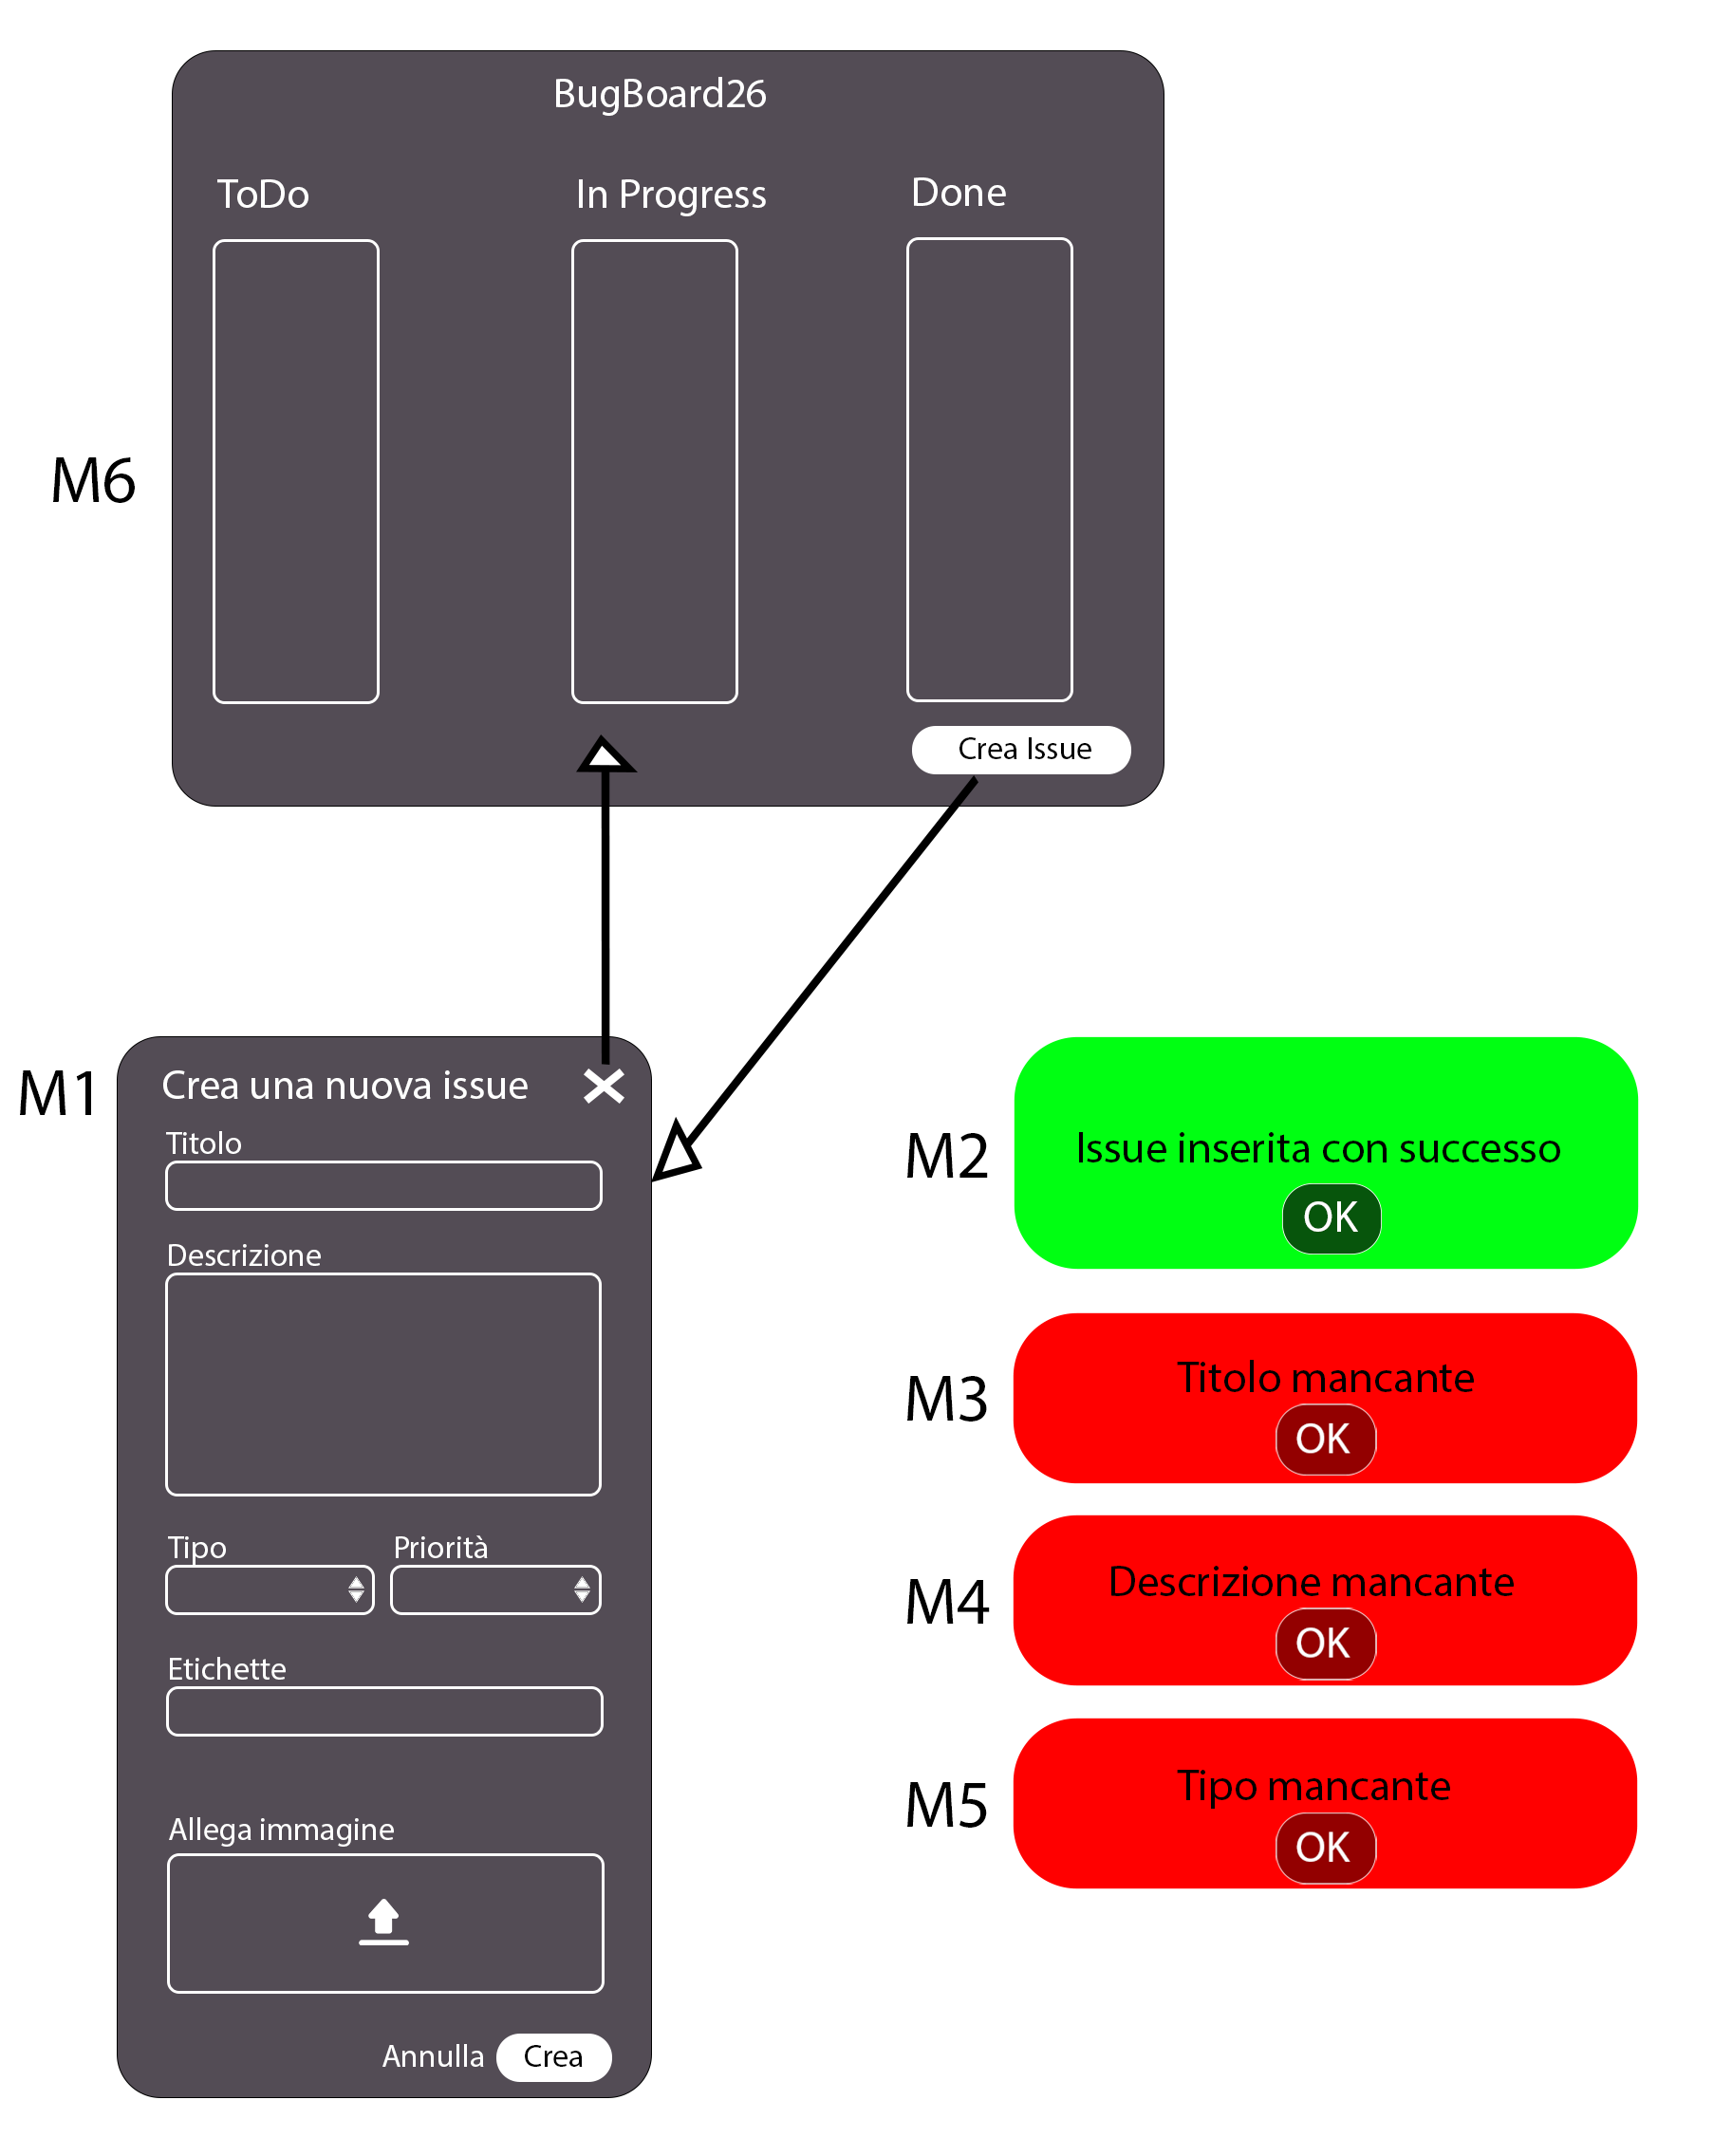
\includegraphics[width=0.7\textwidth]{MOCK.png}
\caption{Mockup flusso creazione issue. La figura mostra:
\textbf{M1} - Form creazione con campi Titolo, Descrizione, Tipo, Priorità, Etichette e Upload immagini;
\textbf{M2} - Messaggio successo "Issue inserita con successo";
\textbf{M3} - Errore "Titolo mancante";
\textbf{M4} - Errore "Descrizione mancante";
\textbf{M5} - Errore "Tipo mancante";
\textbf{M6} - Vista board Kanban con colonne ToDo, In Progress, Done.}
\label{fig:mock-issue}
\end{figure}

% ---------------------------------------------------------------------
\subsubsection{Descrizione Schermate}
\label{subsec:descrizione-schermate}
% ---------------------------------------------------------------------

\paragraph{M1 - Form Creazione Issue}

Form principale per creare nuove issue nel progetto corrente.

\paragraph{Elementi}
\begin{itemize}[leftmargin=1.1em]
\item Header "Crea una nuova issue" con pulsante chiusura (X)
\item Campo Titolo (obbligatorio, input testo singola riga)
\item Campo Descrizione (obbligatorio, textarea multiriga)
\item Dropdown Tipo (obbligatorio: Bug, Feature, Question, Documentation)
\item Dropdown Priorità (opzionale: Nessuna, Bassa, Media, Alta, Critica)
\item Campo Etichette (opzionale)
\item Area upload immagini
\item Pulsanti "Annulla" e "Crea" in basso
\end{itemize}

\paragraph{M2 - Conferma Successo}

Toast notification che appare dopo la creazione con successo della issue.

\subparagraph{Contenuto}
\begin{itemize}[leftmargin=1.1em]
\item Testo "Issue inserita con successo"
\item Pulsante "OK"
\item Scompare automaticamente dopo 3 secondi o al click su OK
\end{itemize}

\subsubsection{M3, M4, M5 - Messaggi Errore}

Alert che appaiono quando mancano campi obbligatori.

\subparagraph{Contenuto}
\begin{itemize}[leftmargin=1.1em]
\item M3: "Titolo mancante"
\item M4: "Descrizione mancante"
\item M5: "Tipo mancante"
\item Pulsante "OK" per chiudere
\item Il campo mancante viene evidenziato in rosso nel form
\end{itemize}

\subsubsection{M6 - Board Kanban}

Vista alternativa delle issue organizzate in colonne per stato.

\subparagraph{Elementi}
\begin{itemize}[leftmargin=1.1em]
\item Header "BugBoard26"
\item Almeno tre colonne: "ToDo", "In Progress", "Done"
\item Pulsante "Crea Issue" in basso a destra
\end{itemize}

\subparagraph{Note}
La board Kanban è una vista alternativa alla lista tabellare, in cui sono presenti colonne corrispettive agli stati con all'interno le varie issue. Le issue possono essere spostate tra colonne con drag\&drop per cambiare lo stato in modo efficiente.

% ---------------------------------------------------------------------
\subsubsection{Principi di Design}
\label{subsec:principi-design}
% ---------------------------------------------------------------------

I mockup seguono questi principi:

\begin{itemize}[leftmargin=1.1em]
\item \textbf{Semplicità}: layout pulito con elementi essenziali
\item \textbf{Feedback immediato}: messaggi di successo/errore chiari
\item \textbf{Validazione}: campi obbligatori evidenziati quando mancanti
\end{itemize}


\newpage
\section{Design del sistema}
% ---------------------------------------------------------------------
\subsection{System Design}
\label{sec:system-design}
% ---------------------------------------------------------------------

Il sistema \productname{} è stato progettato seguendo un'architettura distribuita a tre livelli (three-tier), in cui ciascun componente (front-end, back-end e database) è sviluppato, distribuito e scalato in modo indipendente. Questa scelta architetturale è motivata dalla necessità di garantire \textbf{separazione delle responsabilità}, \textbf{manutenibilità} e \textbf{scalabilità} del sistema nel tempo.

% ---------------------------------------------------------------------
\subsubsection{Criteri di progettazione}
\label{subsec:criteri-progettazione}
% ---------------------------------------------------------------------

Le decisioni architetturali e implementative sono state guidate dai seguenti criteri di design:

\begin{itemize}[leftmargin=1.1em]
\item \textbf{Separazione delle responsabilità (Separation of Concerns)}: ogni componente del sistema ha un ruolo ben definito. Il front-end si occupa esclusivamente della presentazione e dell'interazione con l'utente; il back-end gestisce la logica di business, la validazione e l'accesso ai dati; il database garantisce la persistenza. All'interno del back-end, la logica è ulteriormente stratificata in livelli distinti (Controller, Service, Repository), ciascuno con responsabilità specifiche e non sovrapposte.

\item \textbf{Architettura a livelli (Layered Architecture)}: il back-end adotta un'architettura a livelli conforme ai principi di Spring Boot, in cui ogni strato comunica esclusivamente con quello immediatamente adiacente:
  \begin{itemize}
  \item \textbf{Controller}: riceve le richieste HTTP, effettua la deserializzazione dei parametri e delega l'elaborazione al livello Service. Non contiene logica di business.
  \item \textbf{Service}: implementa la logica applicativa, coordina le operazioni tra più repository e gestisce le regole di business (es.\ controllo permessi, notifiche, validazioni trasversali).
  \item \textbf{Repository}: astrae l'accesso al database tramite il pattern Repository di Spring Data JPA, esponendo metodi di query dichiarativi.
  \item \textbf{Entity}: modella le tabelle del database come classi Java annotate con JPA, definendo relazioni, vincoli e mapping object-relational.
  \end{itemize}

\item \textbf{Data Transfer Objects (DTO)}: la comunicazione tra i livelli e verso il client avviene tramite oggetti DTO dedicati, distinti dalle entity di persistenza. Questo pattern garantisce il \textbf{disaccoppiamento} tra la rappresentazione interna dei dati e la loro esposizione tramite API, consentendo di controllare quali informazioni vengono esposte, evitare dipendenze circolari nella serializzazione e favorire l'evoluzione indipendente del modello dati e delle interfacce REST.

\item \textbf{Architettura component-based (Front-end)}: il front-end è strutturato secondo il paradigma a componenti di React, in cui ogni elemento dell'interfaccia è un componente riutilizzabile e auto-contenuto. L'organizzazione delle directory riflette questa filosofia:
  \begin{itemize}
  \item \texttt{pages/}: componenti di alto livello che rappresentano le viste dell'applicazione (Kanban Board, Progetti, Report, ecc.)
  \item \texttt{components/}: componenti riutilizzabili organizzati per dominio funzionale (\texttt{issues/}, \texttt{projects/}, \texttt{layout/}, \texttt{common/})
  \item \texttt{hooks/}: custom hooks per incapsulare logica riutilizzabile (drag \& drop, responsive detection, theming)
  \item \texttt{context/}: gestione dello stato globale tramite React Context API per autenticazione, progetto corrente e issue
  \item \texttt{api/}: livello centralizzato per le chiamate HTTP tramite Axios, con interceptor per la gestione automatica dei token JWT
  \item \texttt{types/}: definizioni TypeScript per la type safety end-to-end
  \end{itemize}

\item \textbf{Comunicazione REST stateless}: l'interazione tra front-end e back-end avviene tramite API RESTful stateless. Ogni richiesta contiene tutte le informazioni necessarie per essere elaborata (incluso il token JWT di autenticazione), senza che il server mantenga stato di sessione. Questo approccio favorisce la scalabilità orizzontale del back-end.

\end{itemize}
\newpage
% ---------------------------------------------------------------------
\subsubsection{Motivazioni architetturali}
\label{subsec:motivazioni-architetturali}
% ---------------------------------------------------------------------

La scelta di un'architettura three-tier con separazione netta tra i componenti è motivata da diverse considerazioni:

\begin{itemize}[leftmargin=1.1em]
\item \textbf{Manutenibilità}: la stratificazione del codice consente di modificare un livello (ad esempio la logica di business) senza impattare gli altri (presentazione o persistenza), in accordo con il requisito REQ-NFR-05.

\item \textbf{Testabilità}: la separazione in livelli facilita il testing unitario di ciascuno strato in isolamento, grazie alla possibilità di sostituire le dipendenze con mock o stub.

\item \textbf{Riusabilità}: l'organizzazione a componenti (sia lato back-end con i Service che lato front-end con i componenti React) favorisce il riuso della logica in diversi contesti applicativi.

\item \textbf{Sicurezza}: la centralizzazione dell'autenticazione e dell'autorizzazione nel livello back-end, tramite Spring Security, garantisce che le regole di accesso siano applicate uniformemente a tutte le operazioni, indipendentemente dal client che le invoca.

\item \textbf{Evoluzione indipendente}: l'utilizzo di DTO e API REST come contratto tra front-end e back-end consente ai due componenti di evolvere in modo indipendente, purché il contratto venga rispettato.
\end{itemize}


\section{Software Design}
\subsection{Persistenza dei dati}
Per il salvataggio persistente dei dati, abbiamo optato per un database in PostgresSQL.
Siamo partiti dal seguente schema per poi proseguire con una ristrutturazione:
\begin{figure}[H]
    \centering
    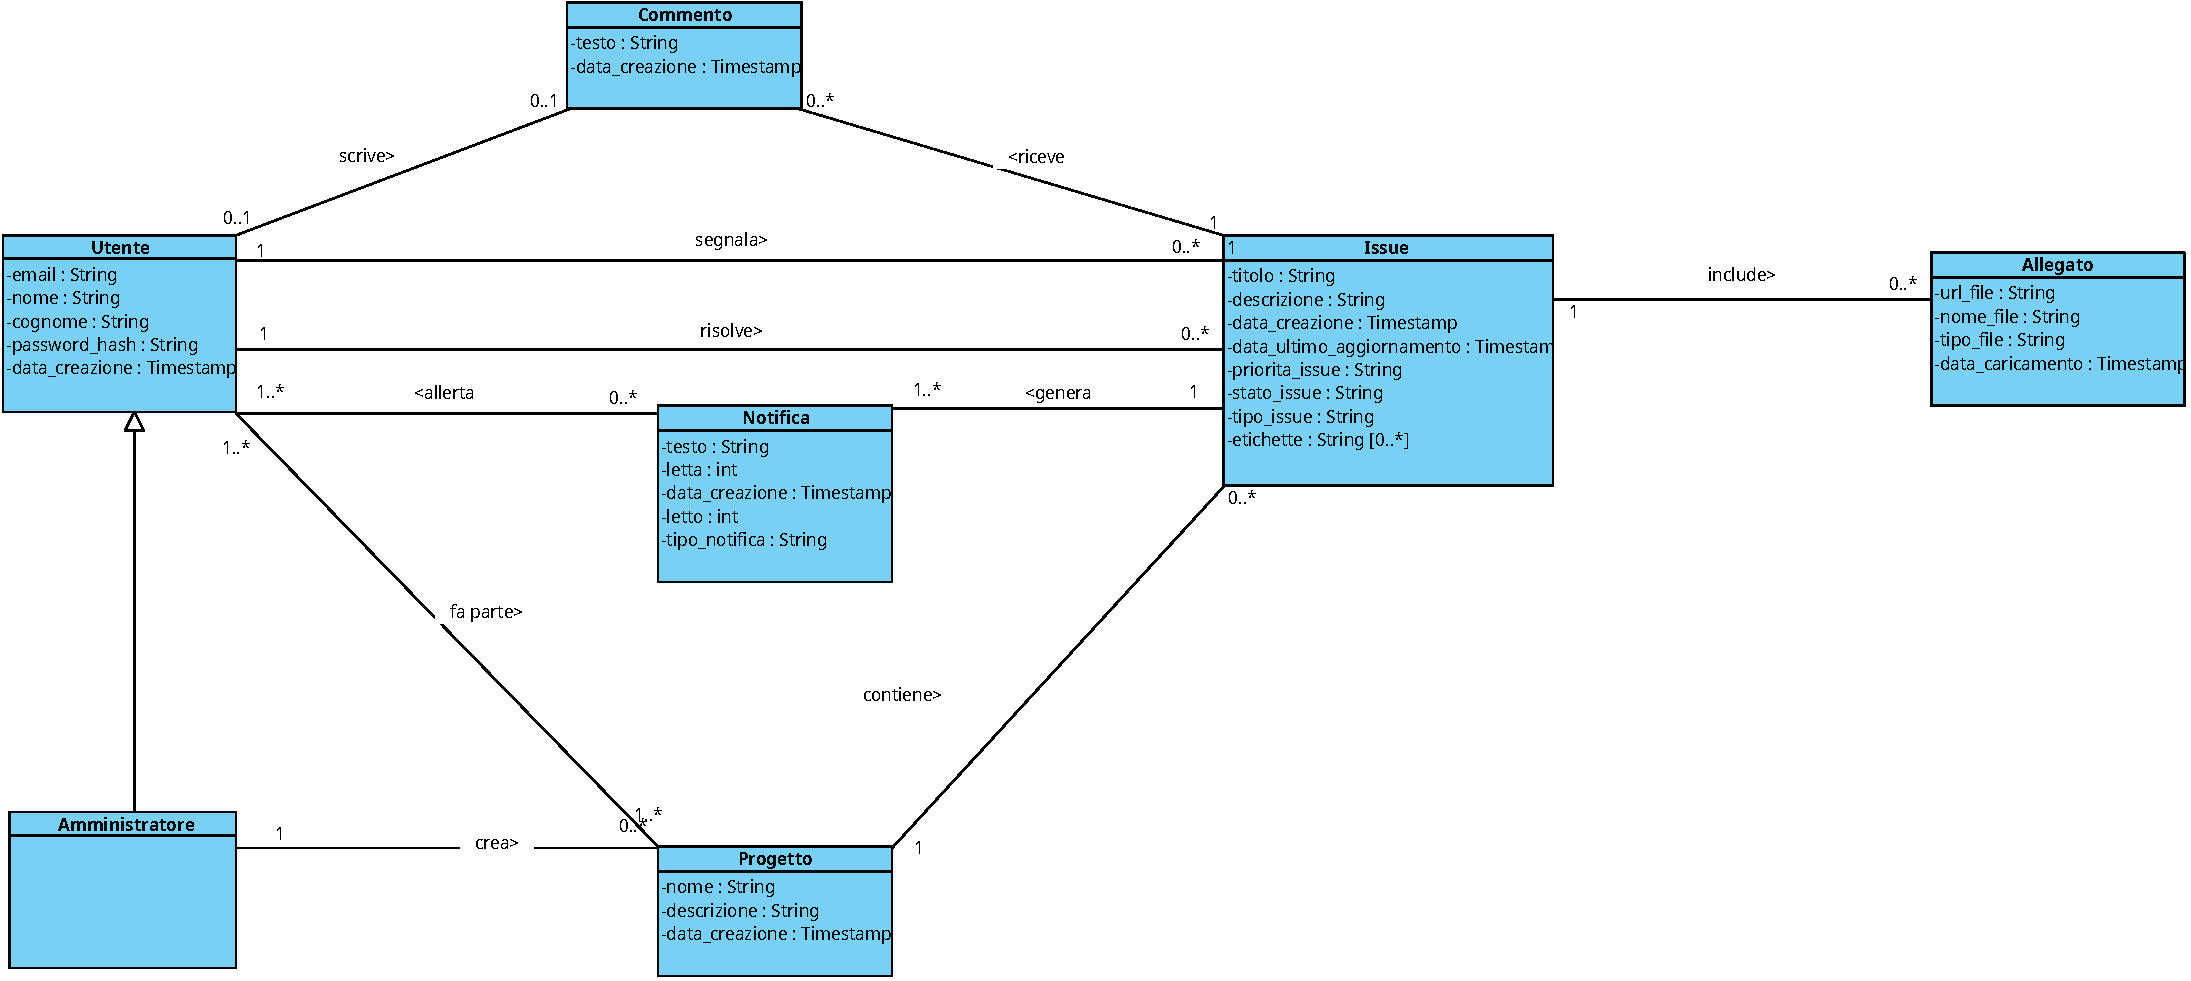
\includegraphics[width=1\textwidth]{DBVECCHIO.pdf}
    \caption{Schema UML}
\end{figure}
\newpage
\subsubsection{Ristrutturazione}
Abbiamo effettuato una ristrutturazione dello schema per migliorarne l'efficienza e prepararlo ad una traduzione in schema logico.
I passaggi effettuati sono stati i seguenti:
\begin{itemize}
    \item \textbf{Analisi delle ridondanze:} abbiamo individuato delle possibili ridondanze nelle associazioni tra utente, amministratore, issue e progetto. Abbiamo tuttavia deciso di mantenerle, data la necessità di effettuare operazioni come ad esempio vedere tutte le issue risolte da un utente, mantenendo queste operazioni semplici attraverso queste associazioni.
    \item \textbf{Eliminazione delle generalizzazioni:} Abbiamo rimosso l'unica generalizzazione presente: quella tra Utente ed Amministratore, accorpando tutto in Utente aggiungendo il campo "ruolo".
    \item \textbf{Eliminazione attributi multivalore:} Abbiamo rimosso l'unico attributo multivalore presente: etichette all'interno di Issue. Abbiamo creato l'entità Etichetta in modo da avere una visione e gestione più chiara delle etichette.
    \item \textbf{Eliminazione attributi strutturati:} Non erano presenti attributi strutturati.
    \item \textbf{Partizionamento/Accorpamento di entità e associazioni:} Non c'è stata necessità di accorpare nulla.
    \item \textbf{Scelta degli identificatori primari:} Per utente abbiamo scelto "email", per tutte le altre entità abbiamo inserito un campo "id".
\end{itemize}
\newpage
L'UML ristrutturato, alla fine, si presenta così:
\begin{figure}[H]
    \centering
    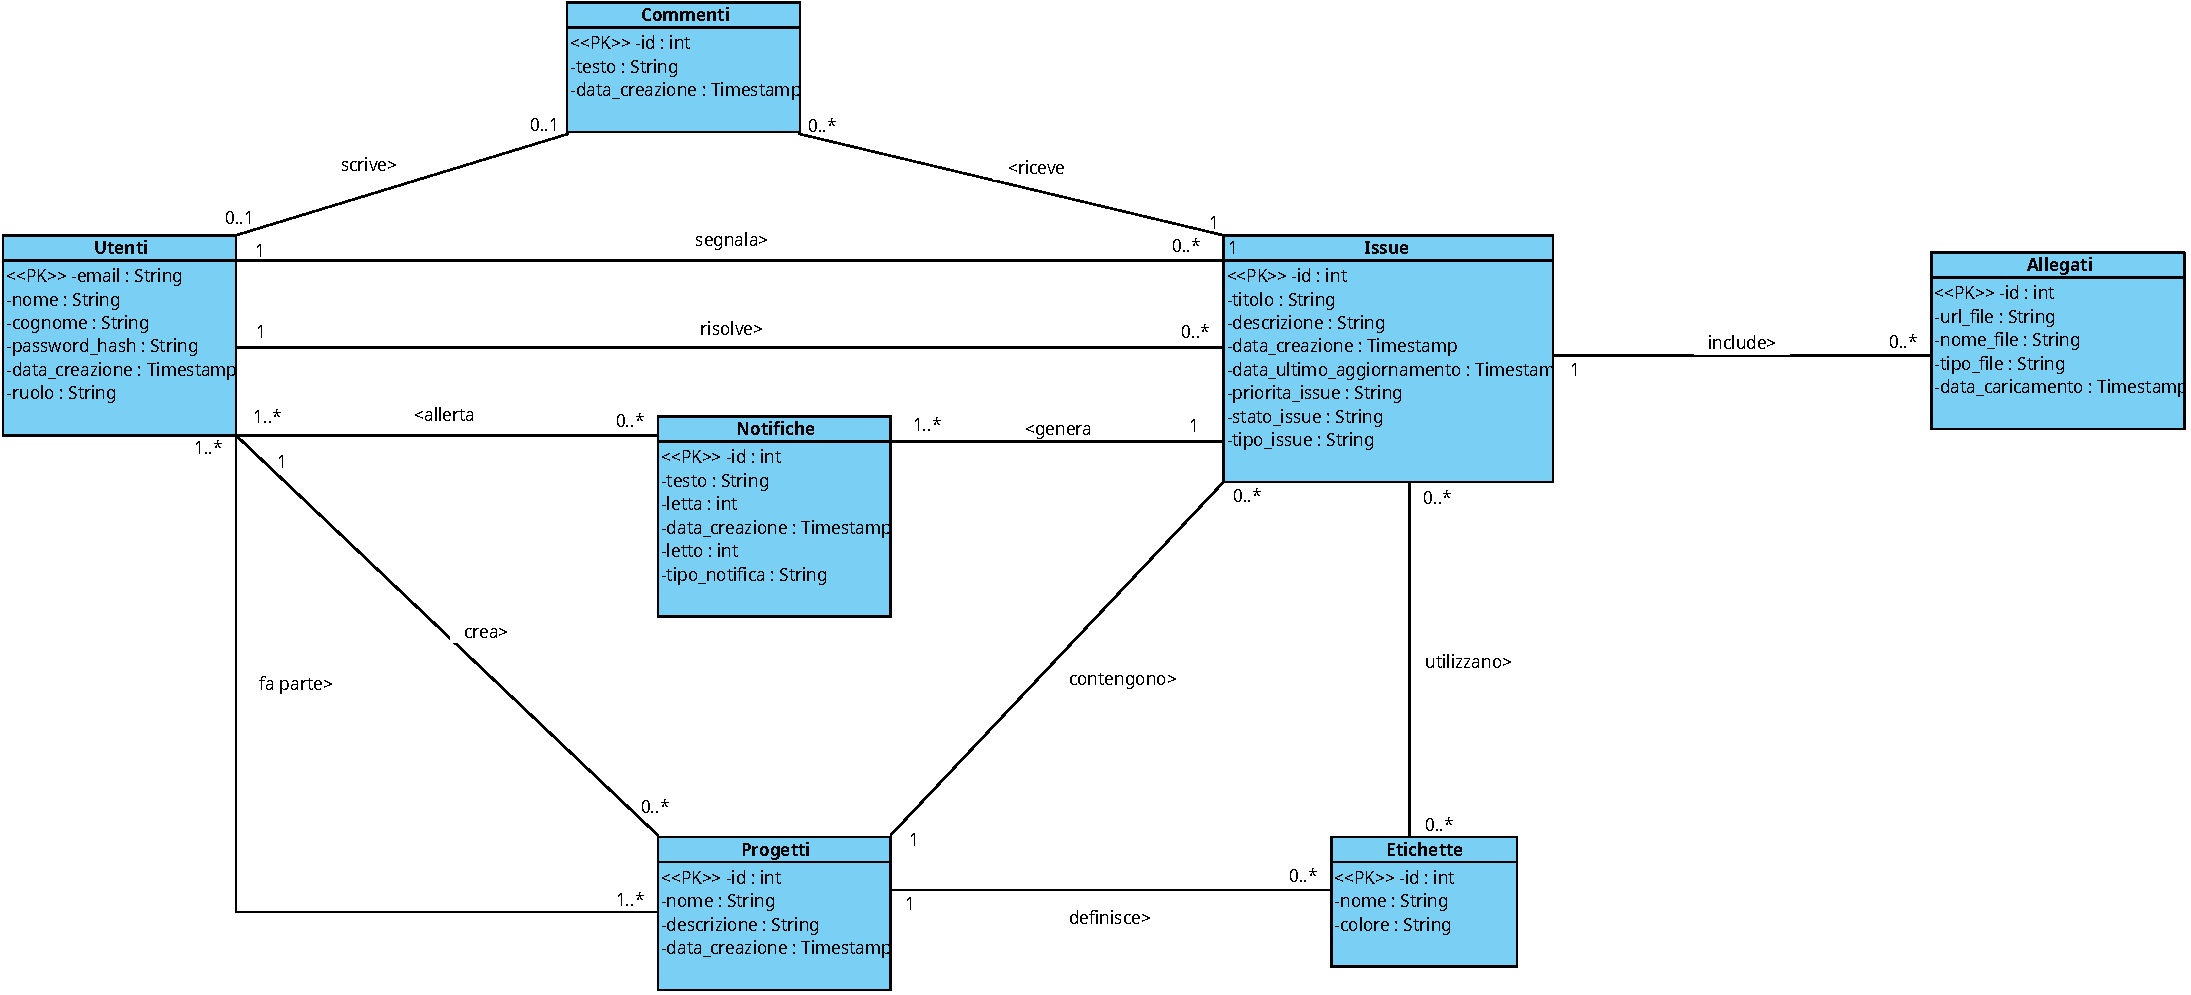
\includegraphics[width=1\textwidth]{DB.pdf}
    \caption{Schema UML ristrutturato}
\end{figure}
\subsubsection{Schema logico}
Lo schema logico derivato dalla ristrutturazione è il seguente:
\begin{itemize}
    \item \textbf{Utente}(\underline{email}, nome, cognome, password\_hash, data\_creazione, ruolo)

    \item \textbf{Progetto}(\underline{id}, nome, descrizione, \underline{\underline{id\_creatore}}, data\_creazione)\\
    \textit{id\_creatore} $\rightarrow$ Utente.email

    \item \textbf{ProgettoMembri}(\underline{\underline{\underline{id\_progetto}}}, \underline{\underline{\underline{email\_utente}}})\\
    \textit{id\_progetto} $\rightarrow$ Progetto.id\\
    \textit{email\_utente} $\rightarrow$ Utente.email

    \item \textbf{Issue}(\underline{id}, \underline{\underline{id\_progetto}}, \underline{\underline{email\_autore}}, \underline{\underline{email\_assegnatario}}, titolo, descrizione, data\_creazione, data\_ultimo\_aggiornamento, priorita\_issue, stato\_issue, tipo\_issue)\\
    \textit{id\_progetto} $\rightarrow$ Progetto.id\\
    \textit{email\_autore} $\rightarrow$ Utente.email\\
    \textit{email\_assegnatario} $\rightarrow$ Utente.email

    \item \textbf{Etichetta}(\underline{id}, \underline{\underline{id\_progetto}}, nome, colore)\\
    \textit{id\_progetto} $\rightarrow$ Progetto.id

    \item \textbf{IssueEtichette}(\underline{\underline{\underline{id\_issue}}}, \underline{\underline{\underline{id\_etichetta}}})\\
    \textit{id\_issue} $\rightarrow$ Issue.id\\
    \textit{id\_etichetta} $\rightarrow$ Etichetta.id

    \item \textbf{Commento}(\underline{id}, \underline{\underline{id\_issue}}, \underline{\underline{email\_autore}}, testo, data\_creazione)\\
    \textit{id\_issue} $\rightarrow$ Issue.id\\
    \textit{email\_autore} $\rightarrow$ Utente.email

    \item \textbf{Allegato}(\underline{id}, \underline{\underline{id\_issue}}, url\_file, nome\_file, tipo\_file, data\_caricamento)\\
    \textit{id\_issue} $\rightarrow$ Issue.id

    \item \textbf{Notifica}(\underline{id}, \underline{\underline{email\_utente}}, \underline{\underline{id\_issue}}, testo, letta, data\_creazione, tipo\_notifica)\\
    \textit{email\_utente} $\rightarrow$ Utente.email\\
    \textit{id\_issue} $\rightarrow$ Issue.id
\end{itemize}

\subsubsection{Funzioni, Trigger \& Varie}

\paragraph{Funzioni}
\begin{itemize}
    \item \textbf{aggiorna\_timestamp\_modifica():} funzione PL/pgSQL che aggiorna automaticamente il campo \texttt{data\_ultimo\_aggiornamento} al timestamp corrente ogni volta che una riga viene modificata.
\end{itemize}

\paragraph{Trigger}
\begin{itemize}
    \item \textbf{trg\_issue\_before\_update:} trigger attivato \texttt{BEFORE UPDATE} sulla tabella \texttt{Issue}. Per ogni riga aggiornata, invoca la funzione \texttt{aggiorna\_timestamp\_modifica()}, garantendo che il campo \texttt{data\_ultimo\_aggiornamento} rifletta sempre l'ultima modifica effettuata.
\end{itemize}

\paragraph{Tipi enumerativi (ENUM)}
Sono stati definiti i seguenti tipi enumerativi per vincolare i valori ammessi in determinati campi:
\begin{itemize}
    \item \textbf{priorita\_issue:} ALTA, BASSA, CRITICA, MEDIA, NESSUNA
    \item \textbf{stato\_issue:} ARCHIVIATA, CHIUSA, IN\_LAVORAZIONE, IN\_REVISIONE, RISOLTA, TODO
    \item \textbf{tipo\_issue:} BUG, DOCUMENTATION, FEATURE, QUESTION
    \item \textbf{tipo\_notifica:} ASSEGNATA, COMMENTO, CRITICA, MENZIONE, PROGETTO, RISOLTA
    \item \textbf{tipo\_ruolo:} AMMINISTRATORE, UTENTE
\end{itemize}

\paragraph{Indici}
Per migliorare le prestazioni delle query più frequenti, sono stati creati i seguenti indici:
\begin{itemize}
    \item \textbf{idx\_utenti\_email} su \texttt{Utente(email)}
    \item \textbf{idx\_progetti\_nome} su \texttt{Progetto(nome)}
    \item \textbf{idx\_progetto\_membri\_utente} su \texttt{ProgettoMembri(email\_utente)}
    \item \textbf{idx\_issue\_progetto} su \texttt{Issue(id\_progetto)}
    \item \textbf{idx\_issue\_assegnatario} su \texttt{Issue(email\_assegnatario)}
    \item \textbf{idx\_commenti\_issue} su \texttt{Commento(id\_issue)}
    \item \textbf{idx\_allegati\_issue} su \texttt{Allegato(id\_issue)}
    \item \textbf{idx\_notifiche\_utente} su \texttt{Notifica(email\_utente)}
    \item \textbf{idx\_notifiche\_letta} su \texttt{Notifica(email\_utente, letta)}
\end{itemize}



\newpage
\subsection{Backend}
Il backend di BugBoard26 è sviluppato in Java con il framework Spring Boot e segue un'architettura a livelli (layered architecture). Il codice è suddiviso nei seguenti package:

\needspace{10\baselineskip}
\subsubsection{Package config}
Qui si trovano le classi di configurazione. La classe \texttt{SecurityConfig} definisce il \texttt{PasswordEncoder} con BCrypt, mentre \texttt{WebSecurityConfig} configura la catena di filtri HTTP con autenticazione Basic, le policy CORS per le richieste dal frontend e le regole di autorizzazione basate sui ruoli (ad esempio, solo gli amministratori possono creare o eliminare utenti).

\begin{figure}[H]
    \centering
    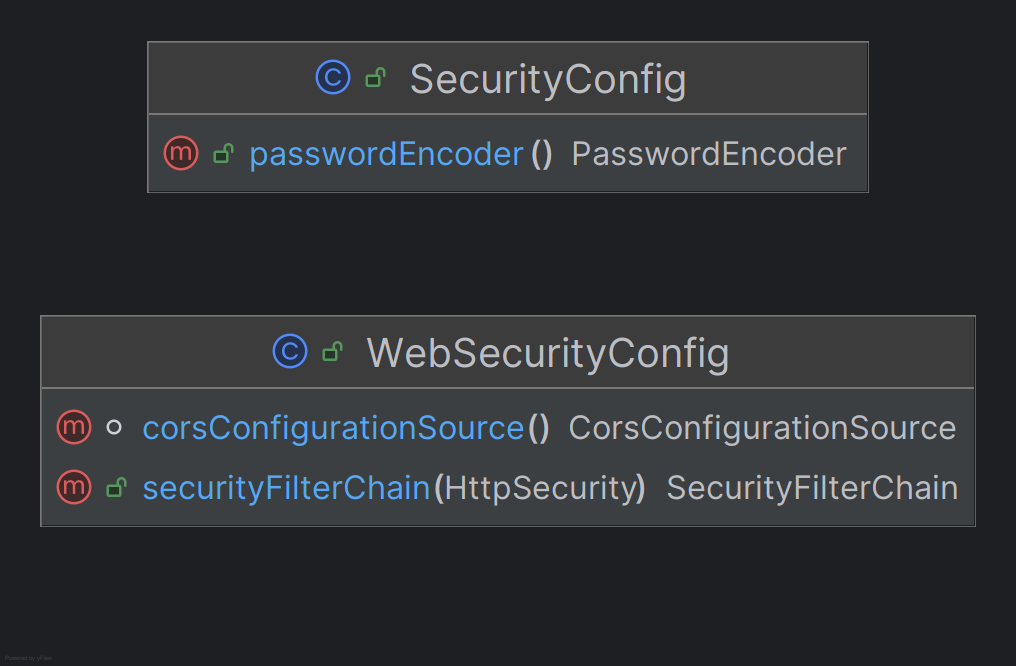
\includegraphics[width=0.6\textwidth]{package config.png}
    \caption{Package diagram del package config}
\end{figure}

\needspace{10\baselineskip}
\subsubsection{Package controller}
Raccoglie i controller REST che espongono le API. Ogni controller corrisponde a una risorsa (utenti, progetti, issue, commenti, allegati, etichette, notifiche) e definisce gli endpoint HTTP (GET, POST, PUT, DELETE) per le operazioni CRUD. Il \texttt{SseController} gestisce le connessioni Server-Sent Events per le notifiche in tempo reale.

\begin{figure}[H]
    \centering
    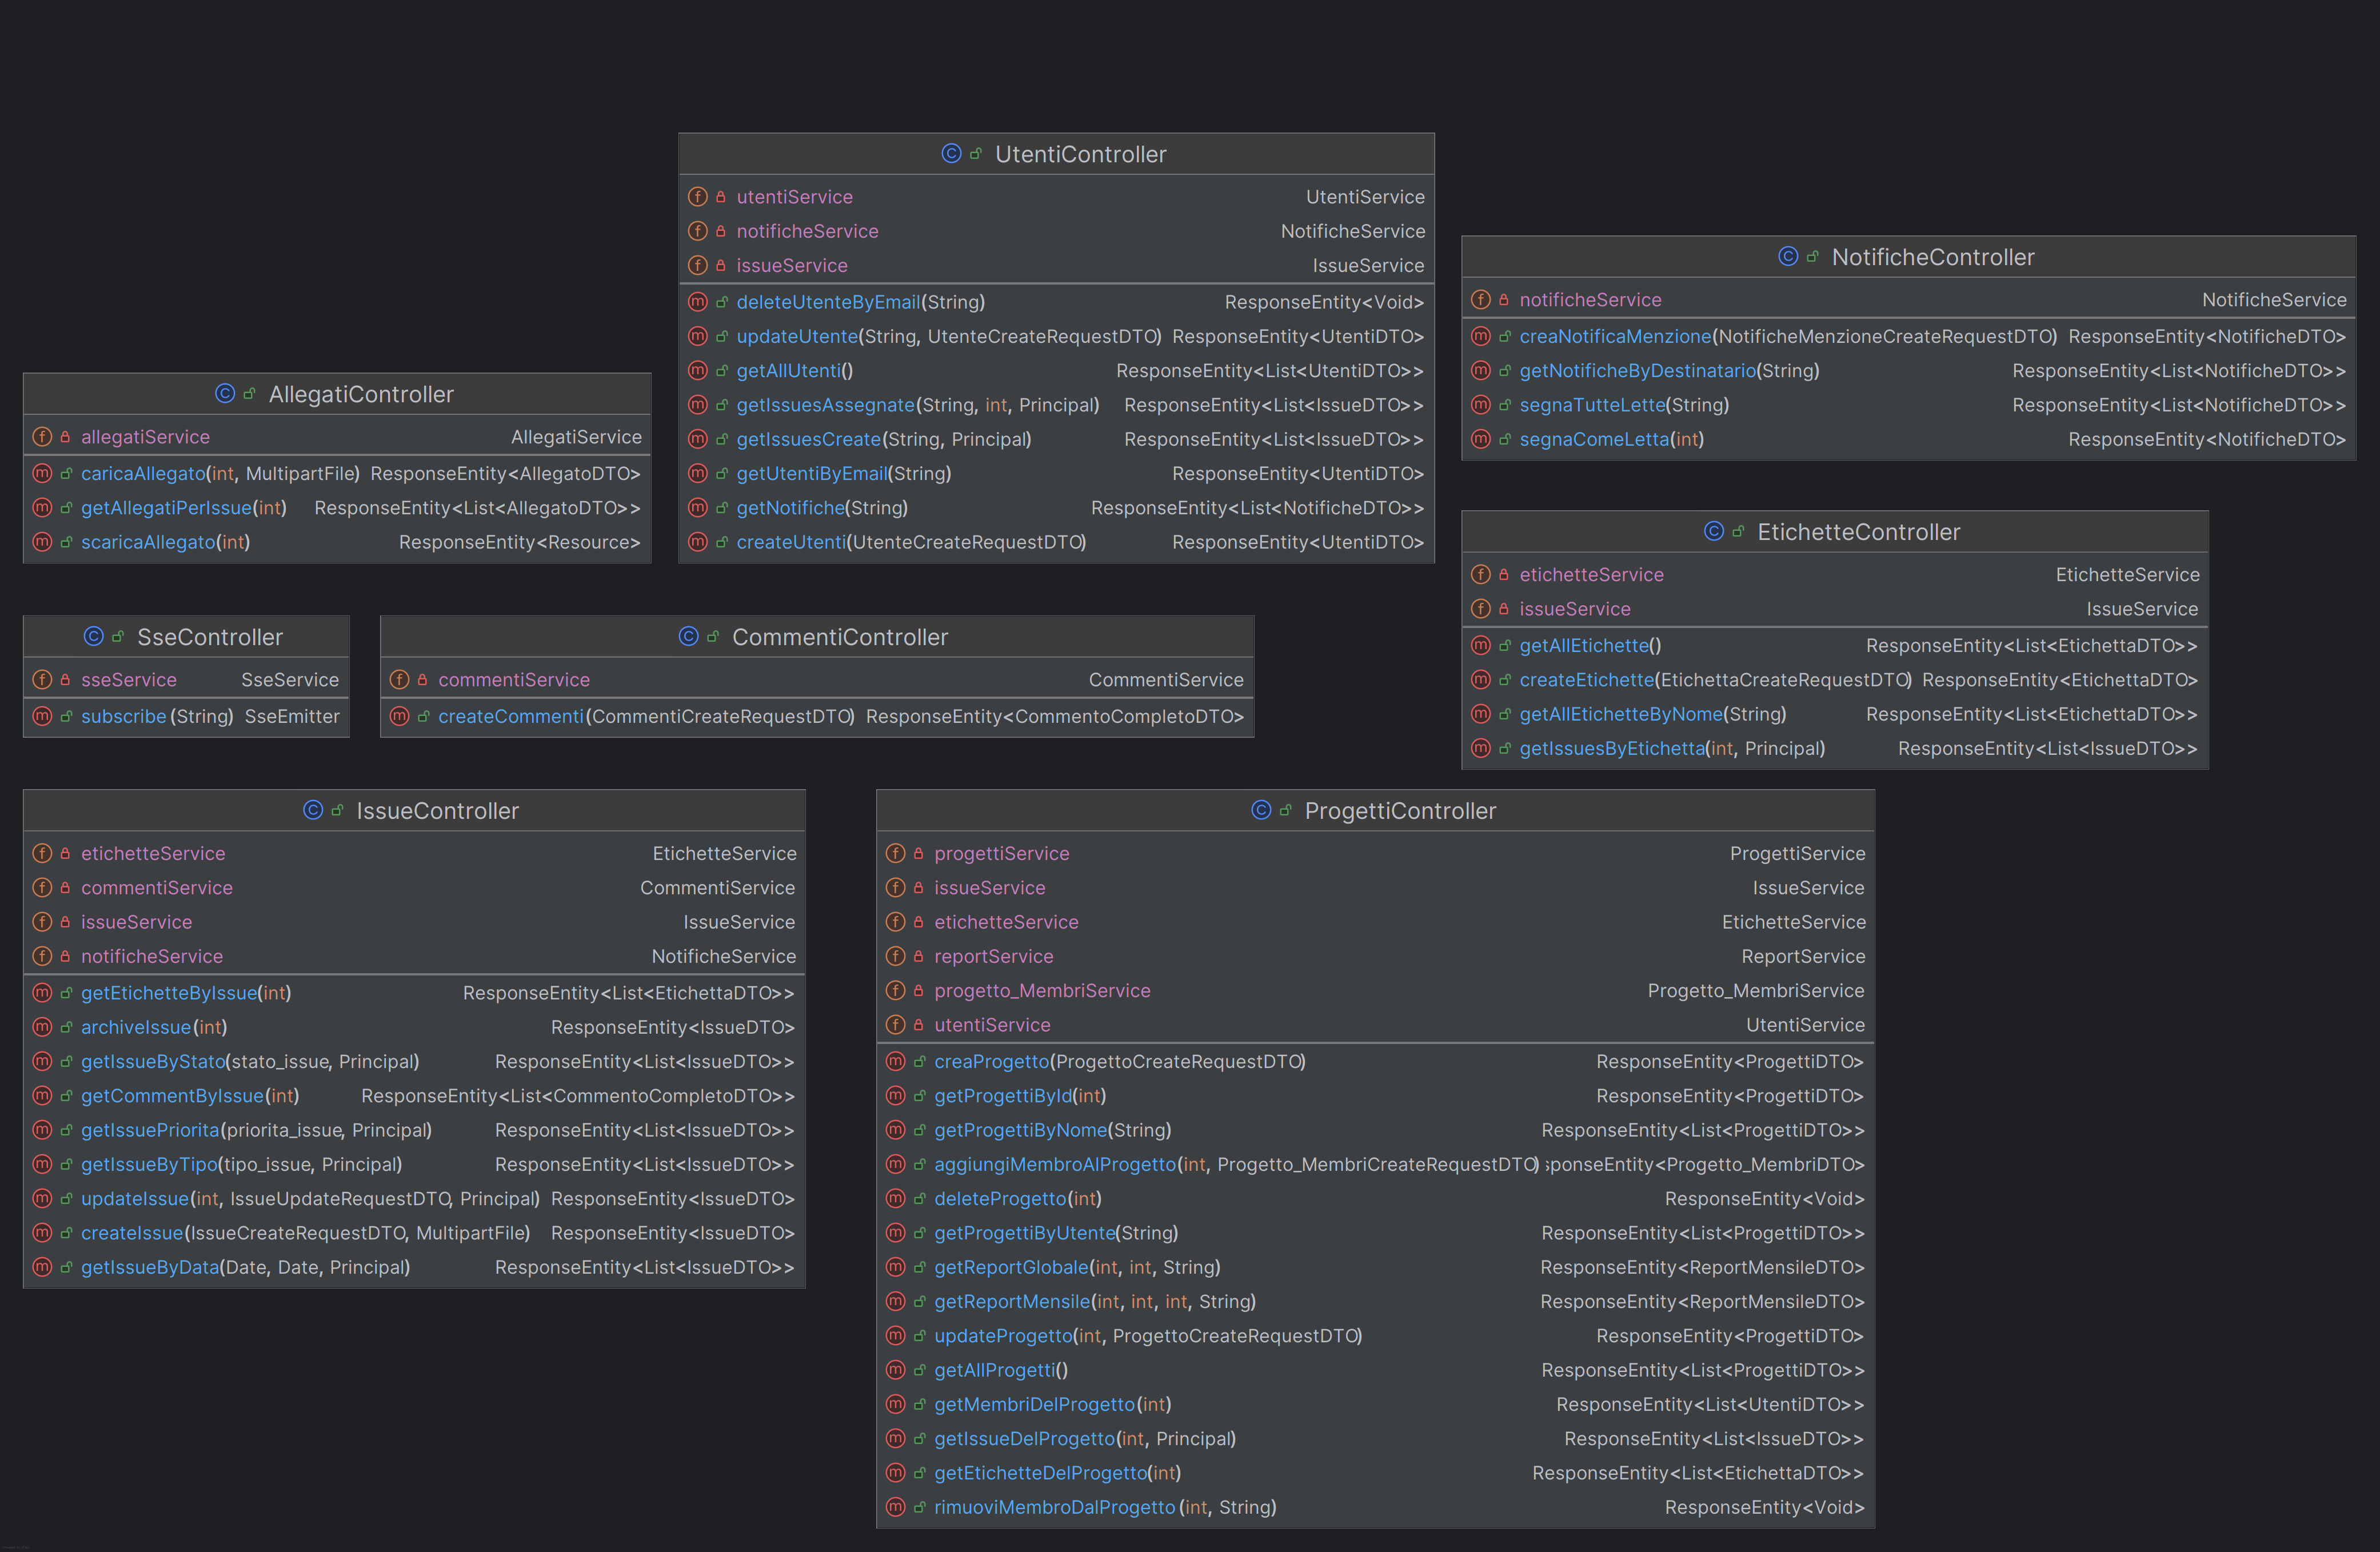
\includegraphics[width=1\textwidth]{package controller.png}
    \caption{Package diagram del package controller}
\end{figure}

\needspace{10\baselineskip}
\subsubsection{Package dto}
Raccoglie i Data Transfer Object (DTO), ovvero classi usate per trasferire dati tra frontend e backend senza esporre direttamente le entità del database. Ci sono DTO di risposta (es.\ \texttt{IssueDTO}, \texttt{UtentiDTO}), DTO di richiesta (es.\ \texttt{IssueCreateRequestDTO}, \texttt{IssueUpdateRequestDTO}) e DTO per i report (\texttt{ReportDTO}, \texttt{ReportMensileDTO}, \texttt{ReportUtenteDTO}).

\begin{figure}[H]
    \centering
    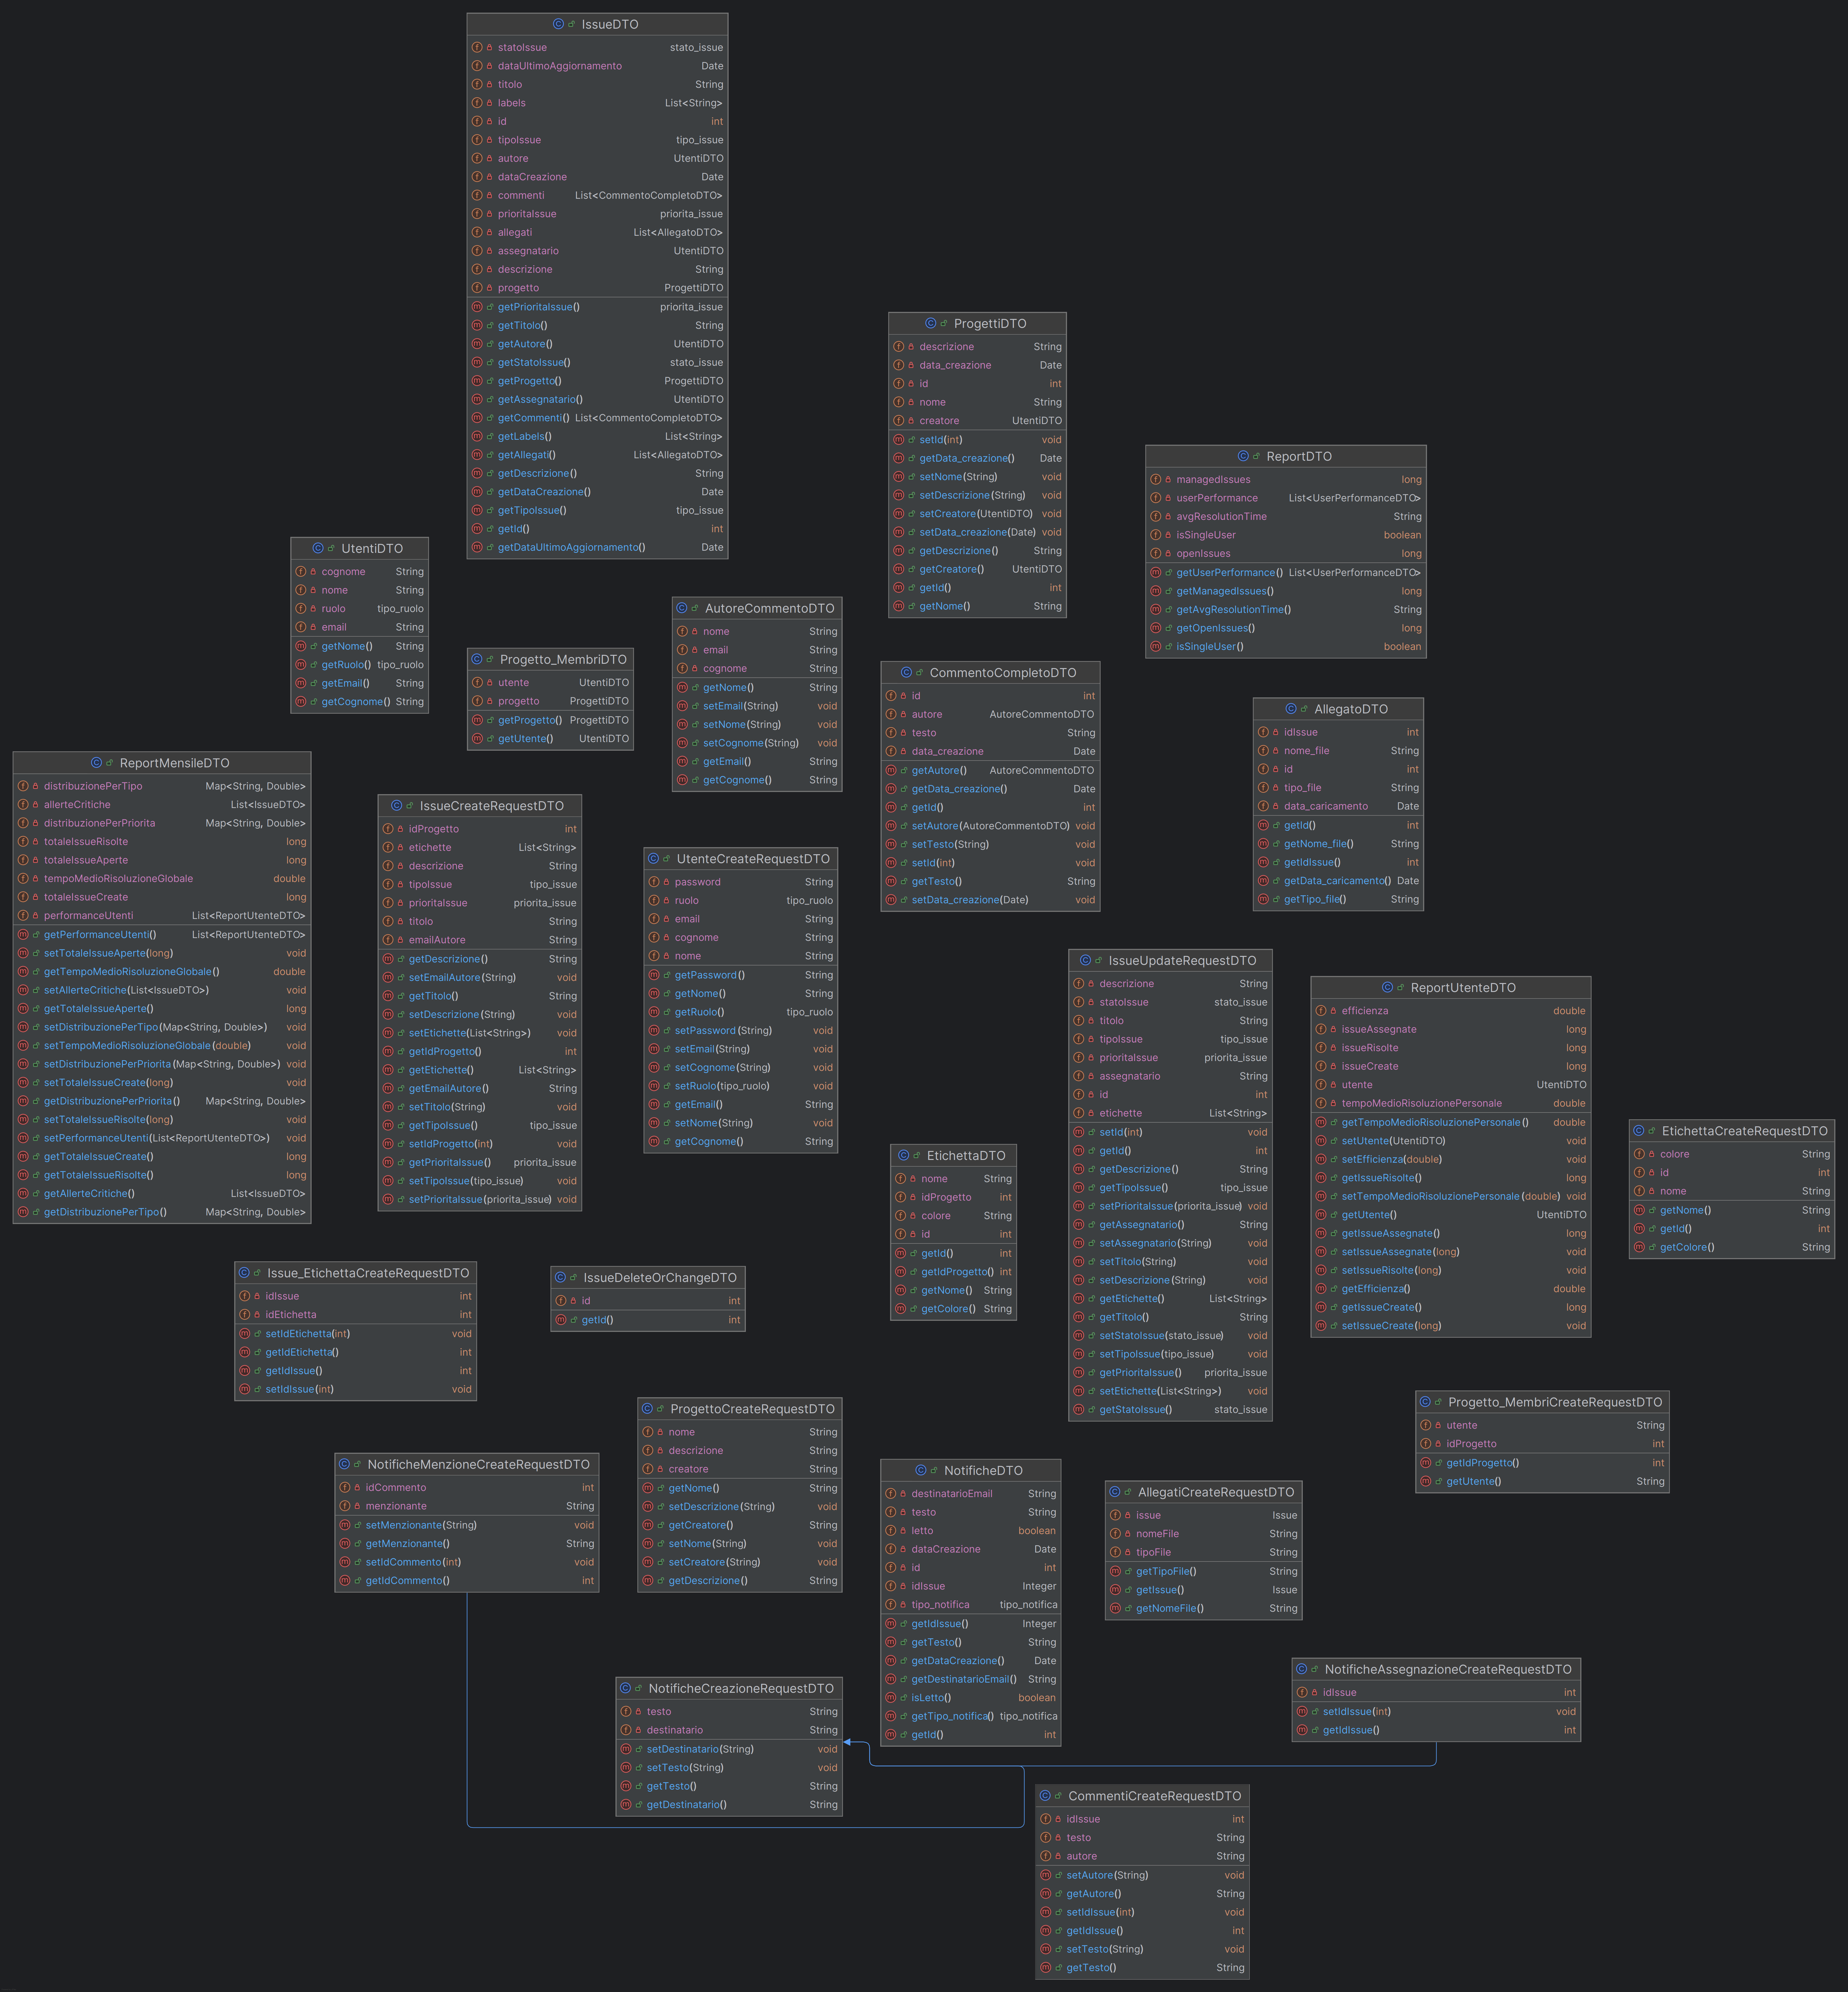
\includegraphics[width=1\textwidth]{package dto.png}
    \caption{Package diagram del package dto}
\end{figure}

\needspace{10\baselineskip}
\subsubsection{Package entity}
Qui ci sono le entità JPA che mappano le tabelle del database. Ogni classe corrisponde a una tabella (es.\ \texttt{Issue}, \texttt{Utenti}, \texttt{Progetti}) con campi, relazioni e vincoli definiti tramite annotazioni JPA. Il sotto-package \texttt{ComposedPrimaryKeys} contiene le chiavi primarie composite (es.\ \texttt{Issue\_EtichettePrimaryKey}, \texttt{Progetto\_MembriPrimaryKey}), mentre \texttt{enumerations} contiene i tipi enumerativi (\texttt{priorita\_issue}, \texttt{stato\_issue}, \texttt{tipo\_issue}, \texttt{tipo\_notifica}, \texttt{tipo\_ruolo}).

\begin{figure}[H]
    \centering
    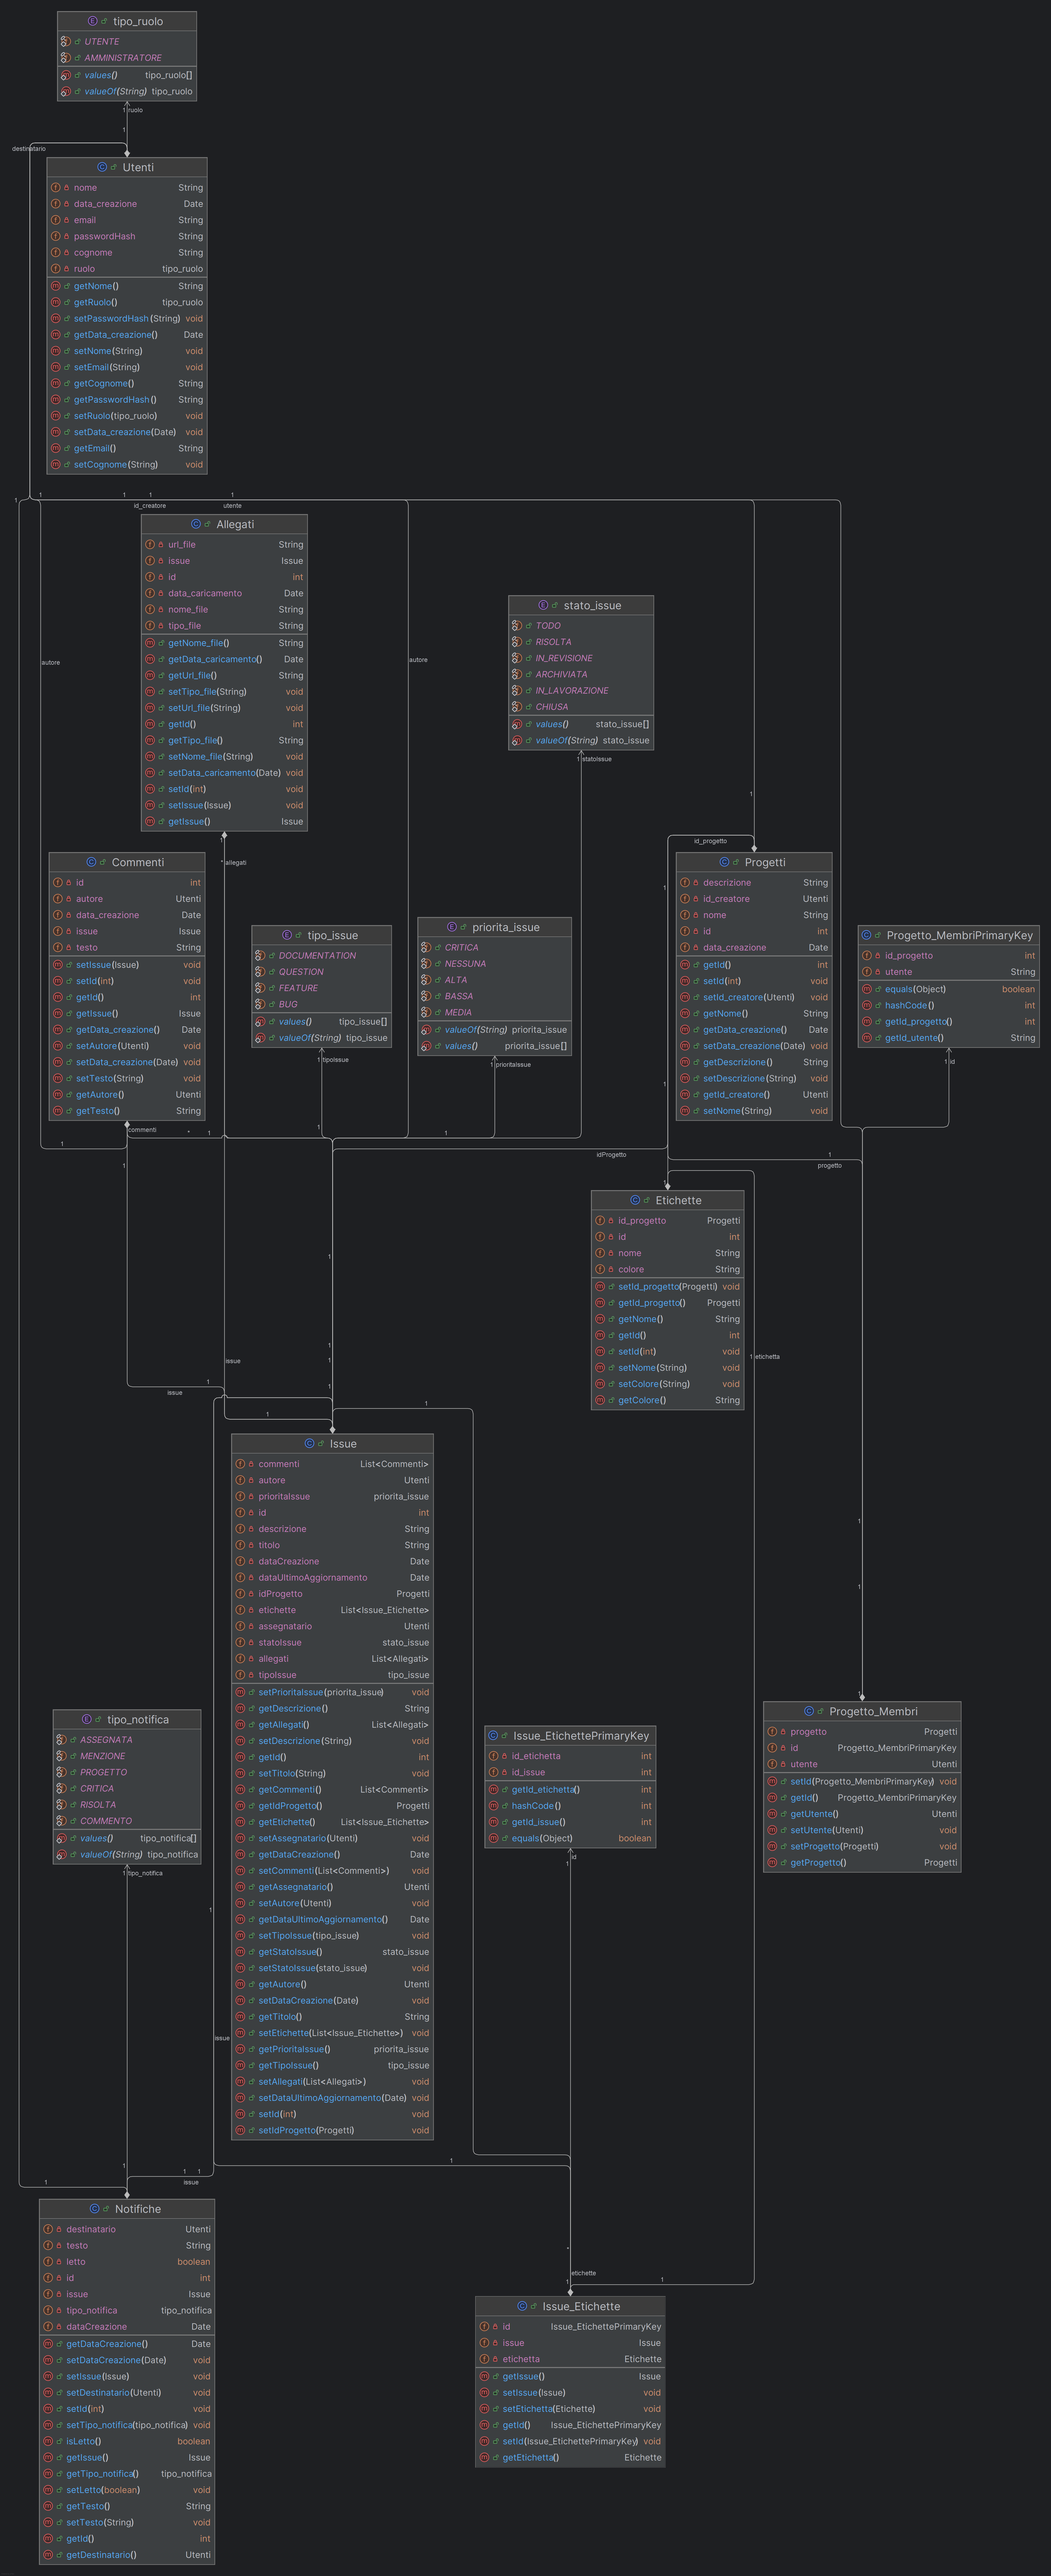
\includegraphics[width=0.5\textwidth]{package entity.png}
    \caption{Package diagram del package entity}
\end{figure}

\needspace{10\baselineskip}
\subsubsection{Package exception}
Contiene le classi per la gestione degli errori e le eccezioni personalizzate (come \texttt{ResourceNotFoundException} o \texttt{BadRequestException}). Invece di far gestire i problemi ai singoli componenti, la classe \texttt{GlobalExceptionHandler} cattura le eccezioni a livello globale e le converte in risposte HTTP standardizzate e coerenti per il frontend.

\begin{figure}[H]
    \centering
    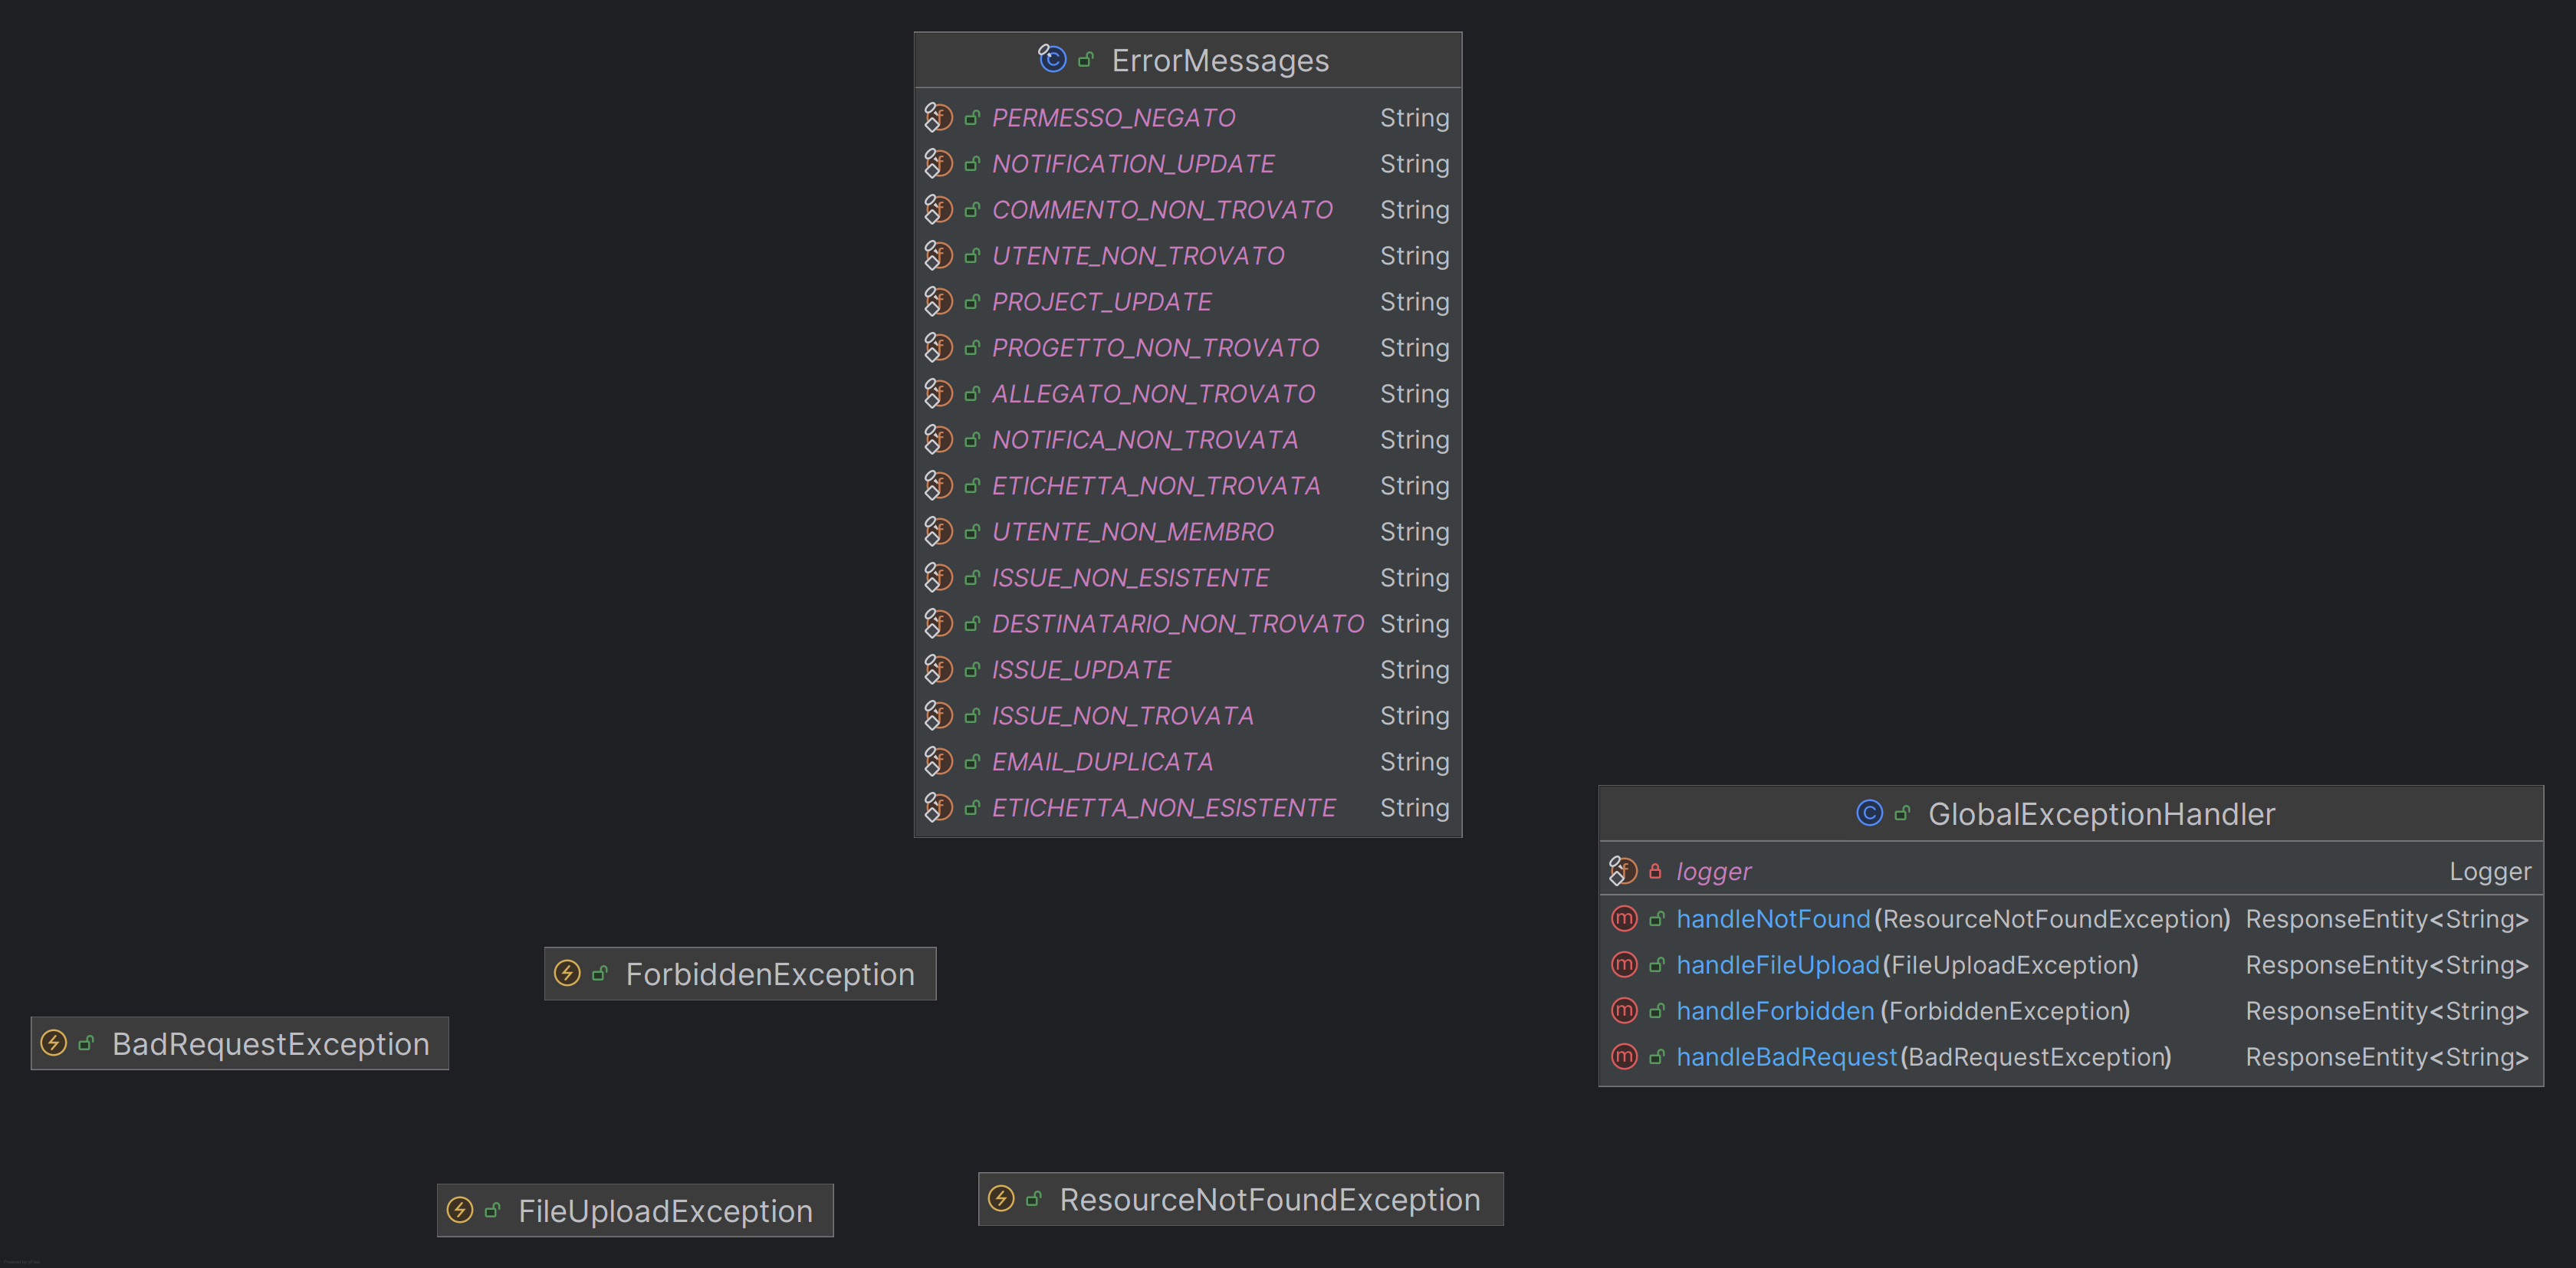
\includegraphics[width=0.8\textwidth]{package extensions.png}
    \caption{Package diagram del package exception}
\end{figure}

\needspace{10\baselineskip}
\subsubsection{Package repository}
Raccoglie le interfacce repository che estendono \texttt{JpaRepository} di Spring Data JPA. Ogni repository è legato a un'entità e fornisce i metodi per l'accesso ai dati, sia query CRUD predefinite che query personalizzate. C'è un repository per ogni entità: utenti, progetti, membri dei progetti, issue, etichette, associazioni issue-etichette, commenti, allegati e notifiche.

\begin{figure}[H]
    \centering
    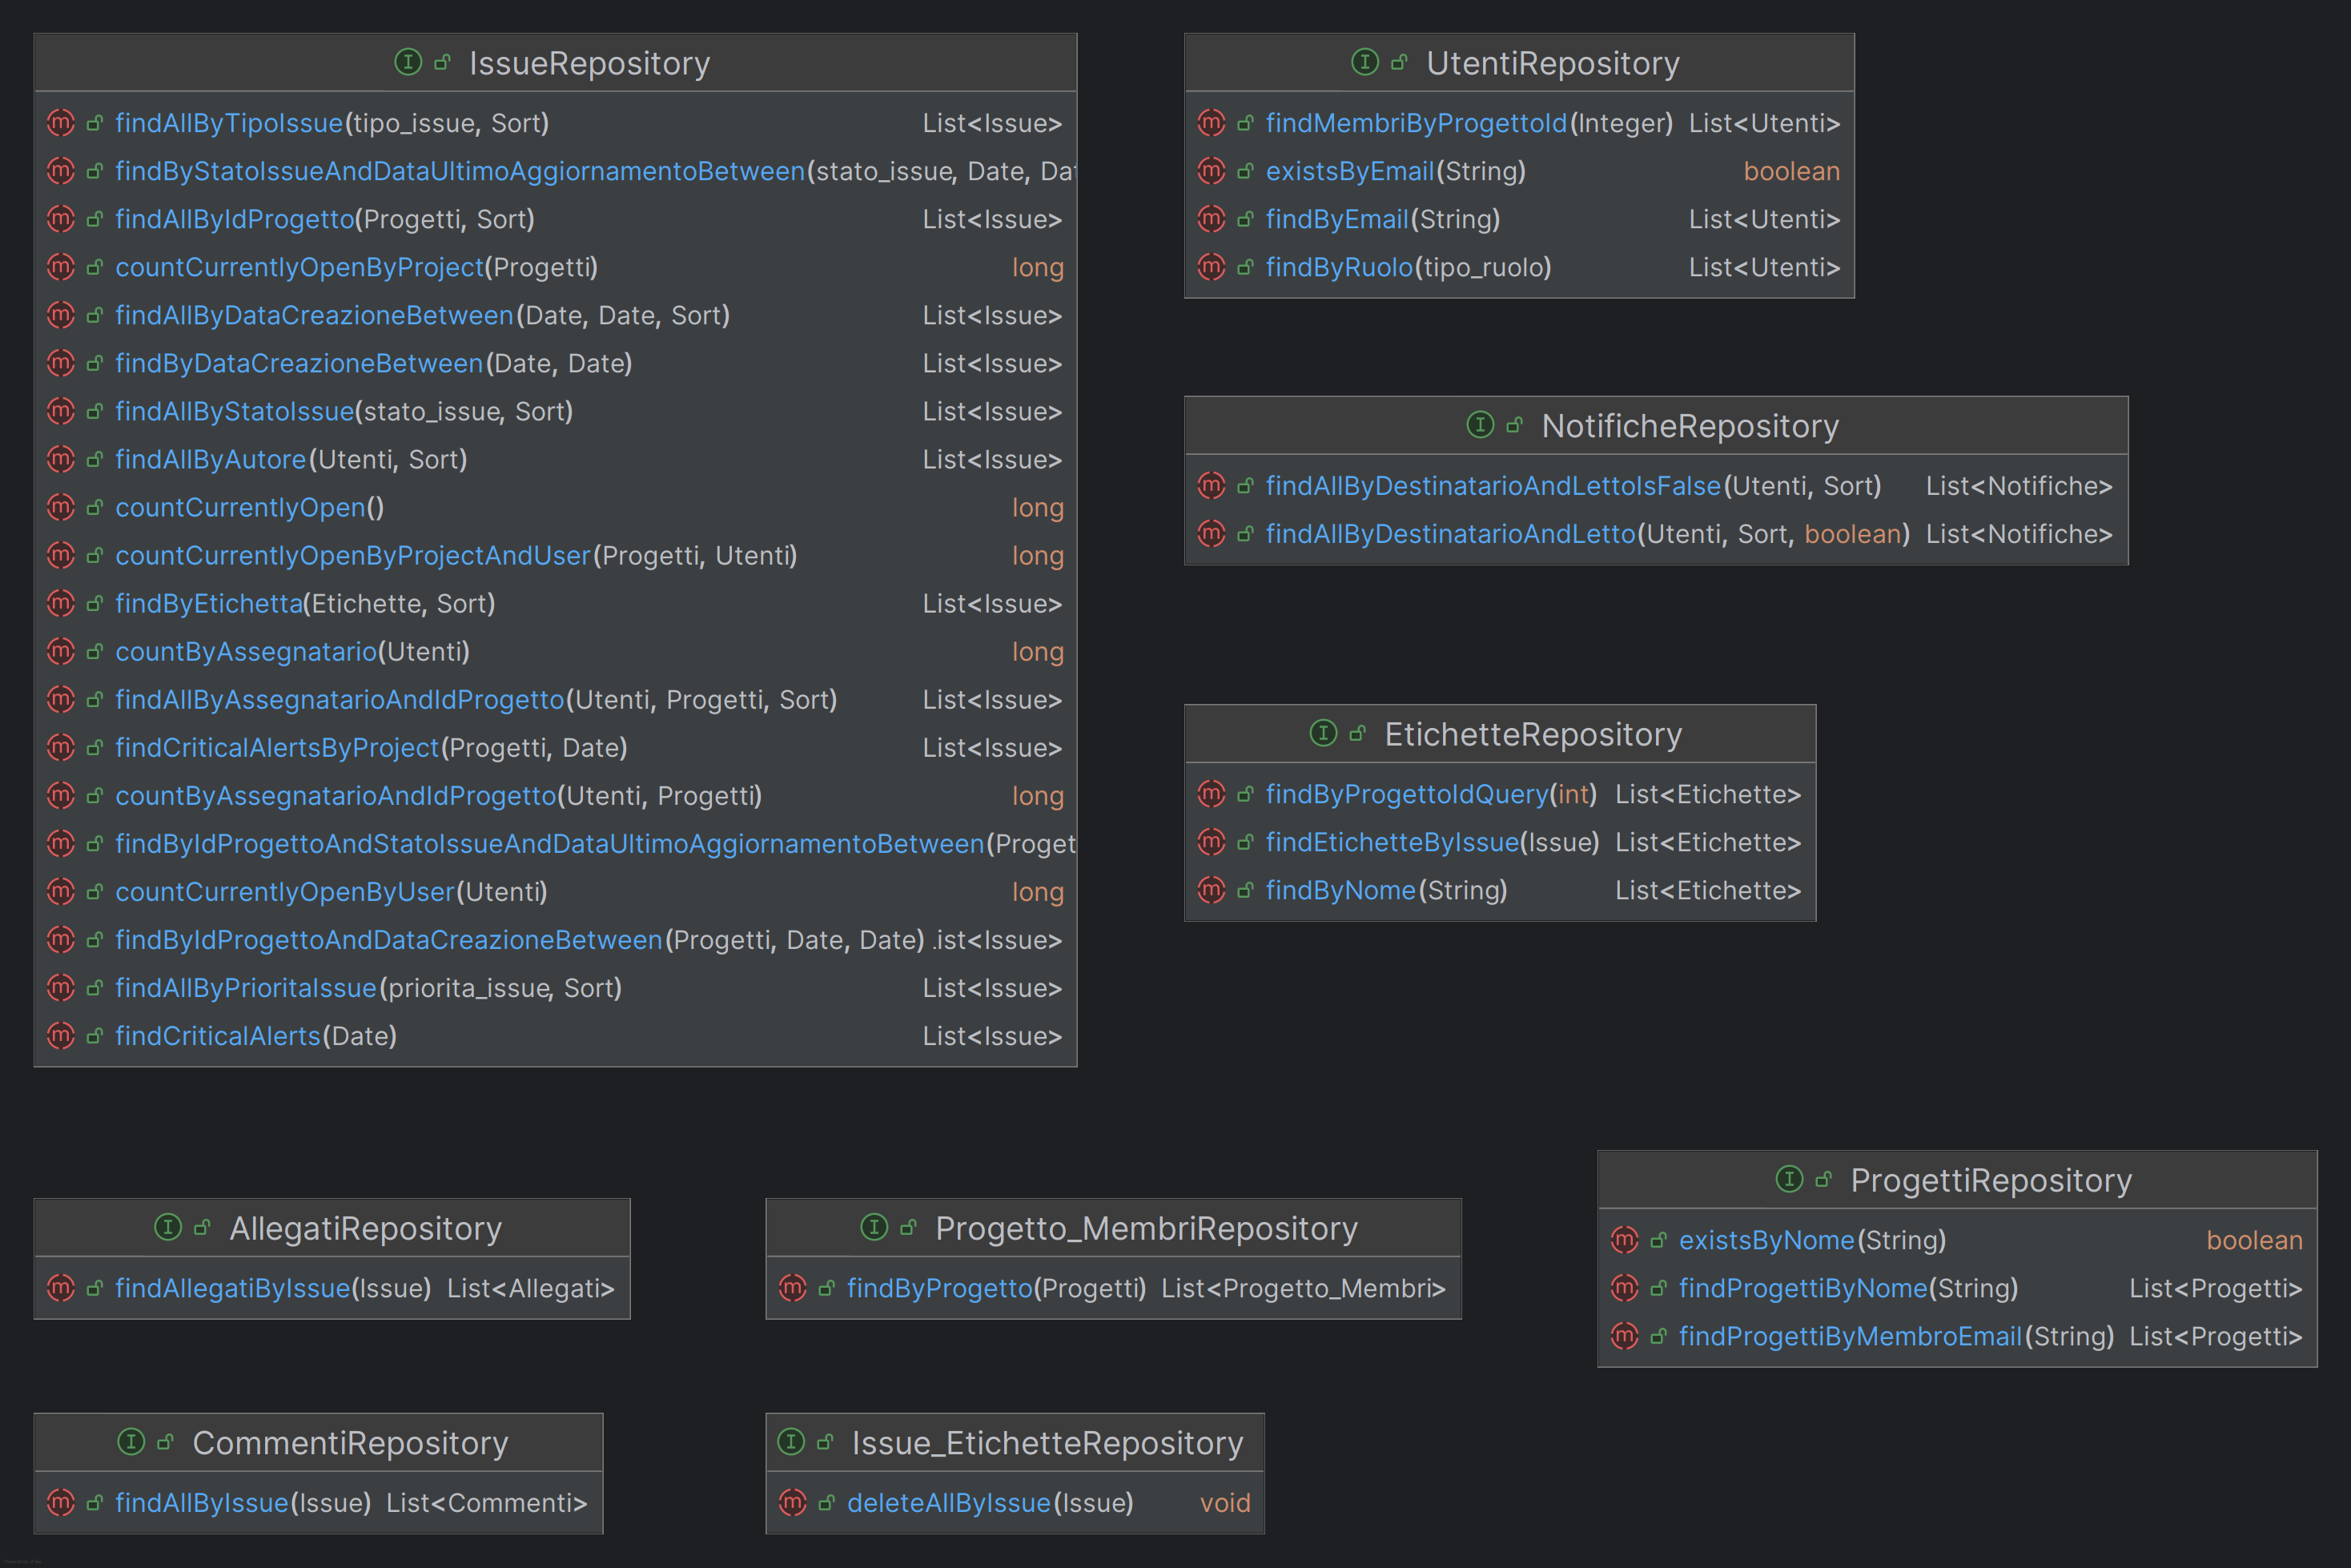
\includegraphics[width=1\textwidth]{package repository.png}
    \caption{Package diagram del package repository}
\end{figure}

\newpage
\subsubsection{Package service}
Raccoglie le classi di servizio con la logica di business. Ogni service si interpone tra il controller e il repository, occupandosi della validazione dei dati, delle trasformazioni tra entità e DTO, e delle operazioni che coinvolgono più entità. Il \texttt{SseService} gestisce le notifiche in tempo reale tramite Server-Sent Events, mentre il \texttt{ReportService} si occupa della generazione di statistiche.

\begin{figure}[H]
    \centering
    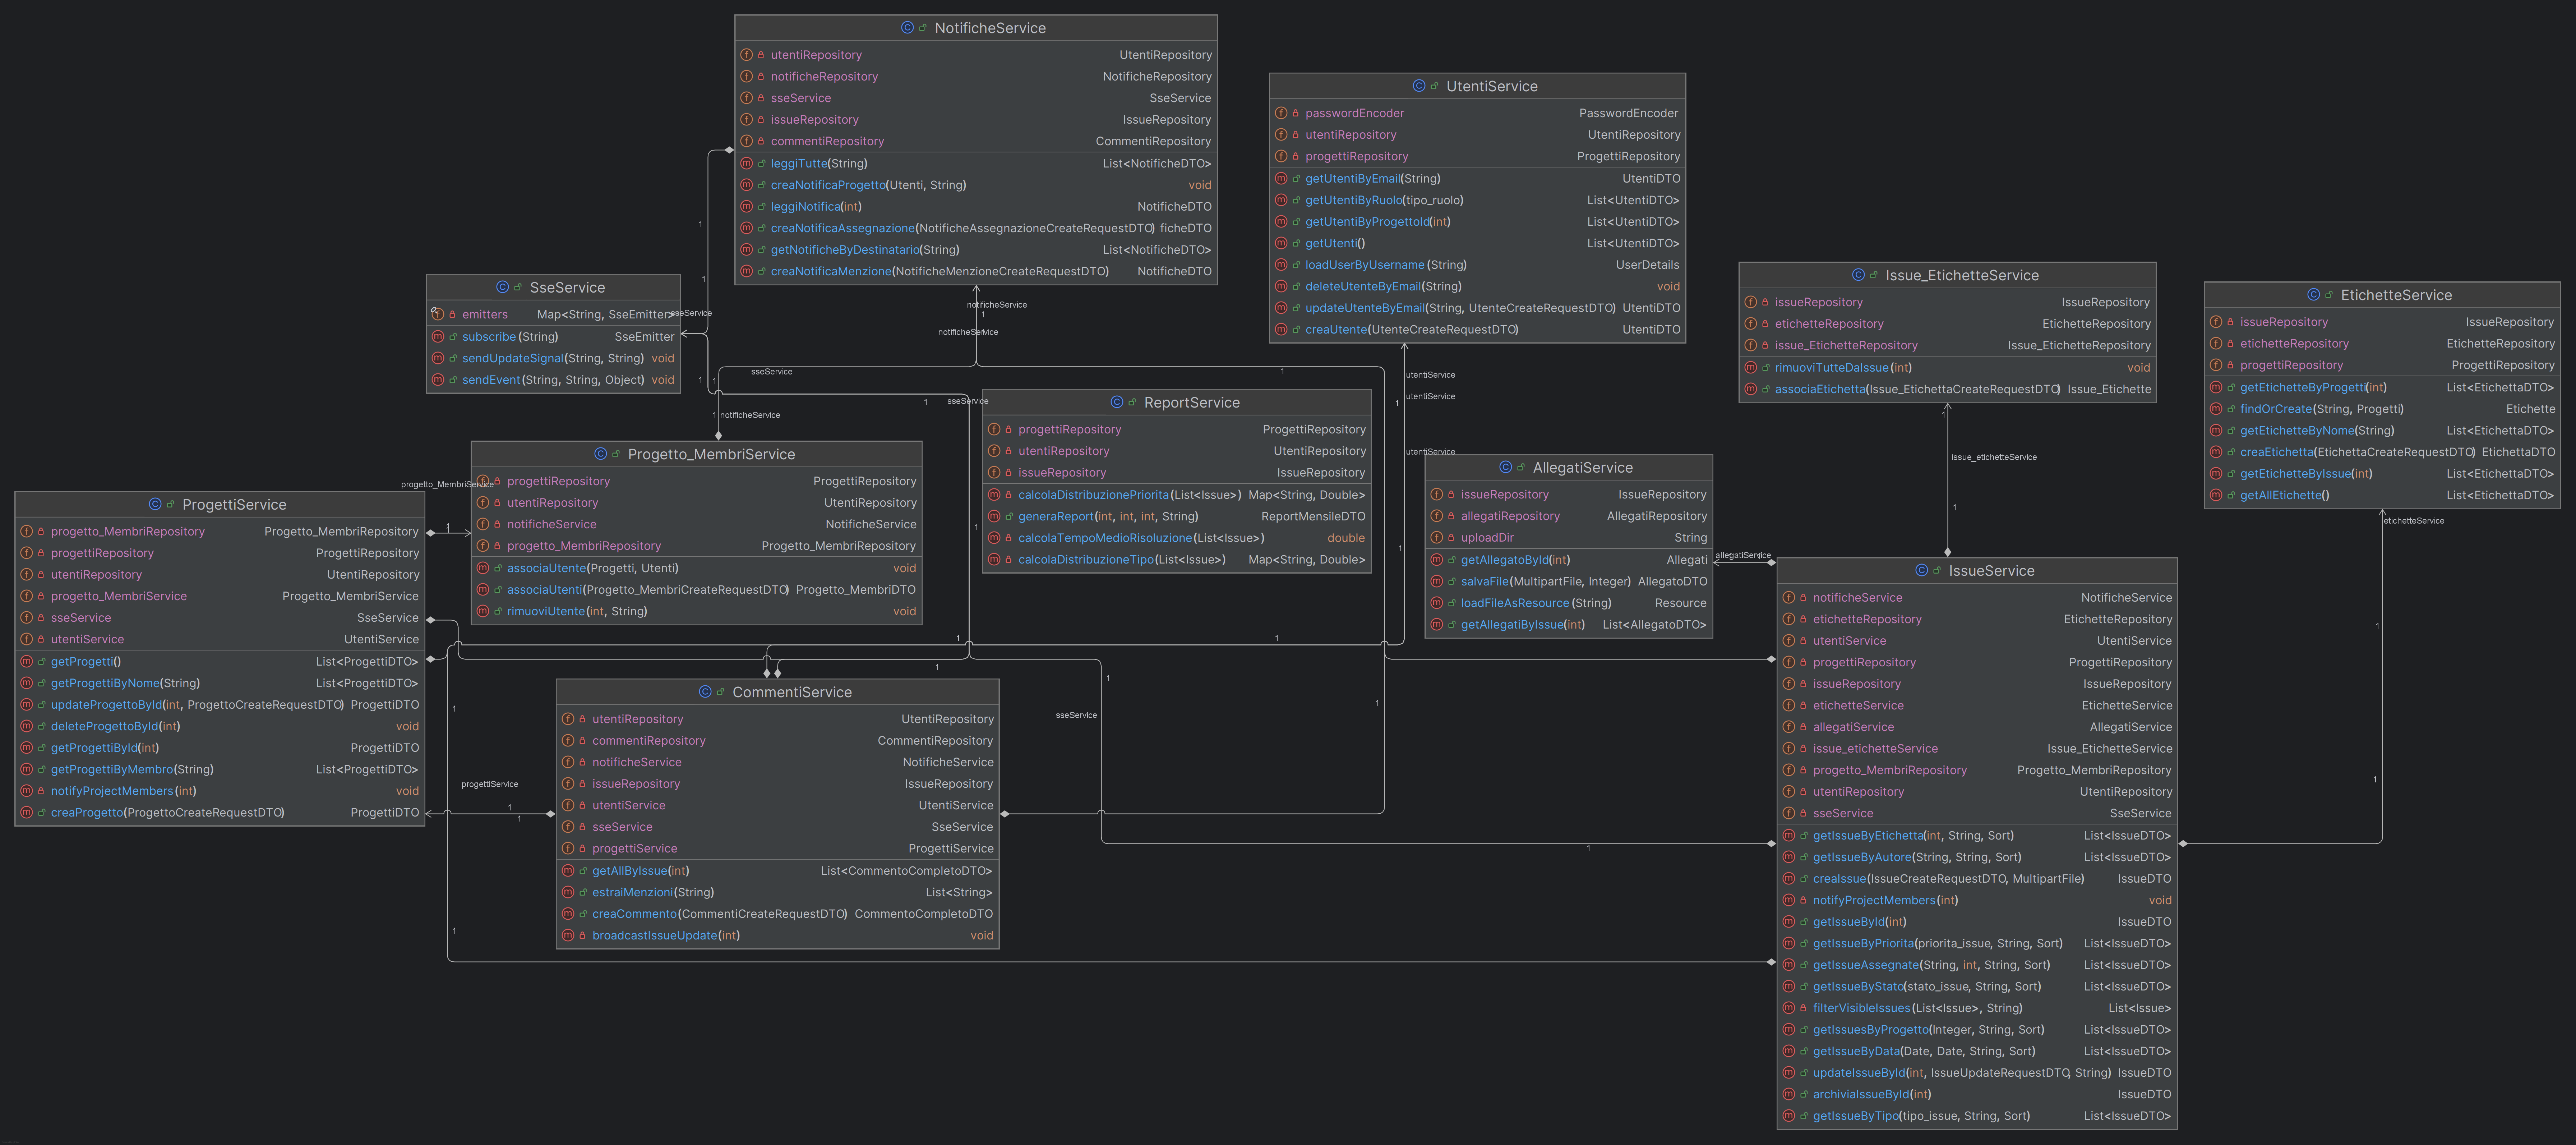
\includegraphics[width=1\textwidth]{package service.png}
    \caption{Package diagram del package service}
\end{figure}
\newpage

\subsection{Frontend}

Anche se nel diagramma utilizziamo una notazione simile alle classi, il frontend in React è costruito quasi esclusivamente con componenti funzionali. Il codice è organizzato per tenere ben separate la grafica dalla pura logica. I componenti visivi sono divisi per area funzionale (le issue, i progetti, o gli utenti) ed esistono poi librerie di elementi base condivisi (come bottoni, finestre modali o il layout generale).

Per evitare di avere componenti React enormi e illeggibili, abbiamo spostato il "lavoro sporco" in file dedicati:
\begin{itemize}
    \item \textbf{Servizi API:} file che fanno esclusivamente chiamate HTTP al backend, gestendo al loro interno gli URL e gli eventuali errori di rete.
    \item \textbf{Context React:} contenitori globali che tengono in memoria dati condivisi (ad esempio chi è l'utente connesso al momento), in modo che chiunque ne abbia bisogno nell'app possa accedervi direttamente.
    \item \textbf{Hook personalizzati:} pezzi di logica legati allo stato che ci capita di riutilizzare in più punti, come ad esempio la gestione di un caricamento asincrono.
\end{itemize}

Così facendo, la maggior parte dei componenti React si preoccupa soltanto di mostrare i dati a schermo e di reagire ai click dell'utente, delegando tutto il recupero e l'aggiornamento dei dati ai context e ai service.

\begin{figure}[H]
    \centering
    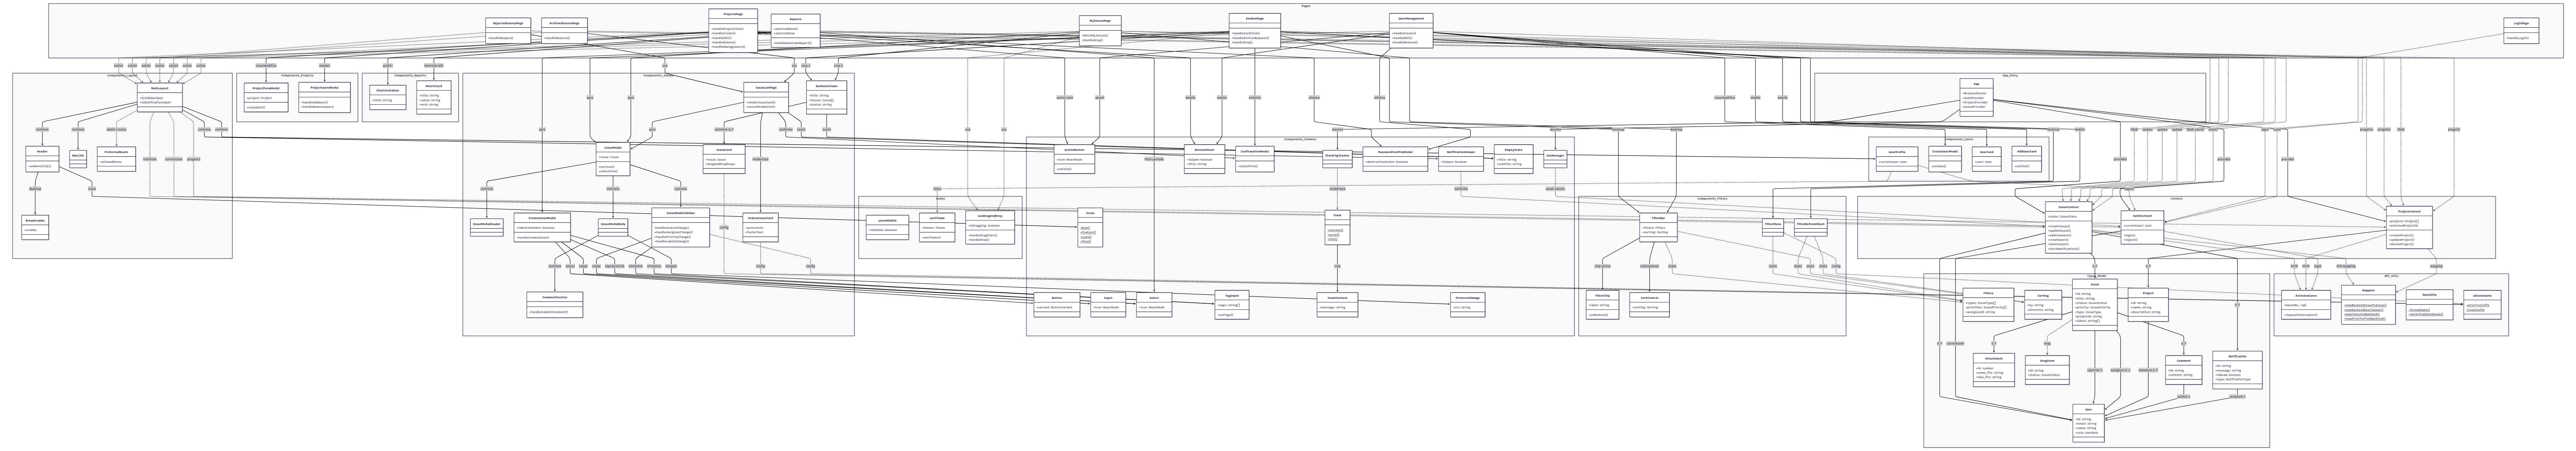
\includegraphics[width=1\textwidth]{ui_completo_bb26.png}
    \caption{Schema del front end}
\end{figure}

\newpage
\subsection{Scelte di design}

Il progetto BugBoard26 è stato strutturato per essere facile da mantenere e da estendere. Per fare ciò, sia nel backend che nel frontend abbiamo seguito i principi SOLID e alcuni design pattern fondamentali.

\subsubsection{Backend}

Il backend in Java e Spring Boot usa un'architettura a livelli (controller, service, repository, entity), in modo da tenere separate le diverse responsabilità e semplificare il collaudo delle singole parti.

\paragraph{Principio di Singola Responsabilità (SRP)}
Abbiamo diviso i compiti rigidamente: i controller gestiscono solo le chiamate HTTP, i service contengono tutta la logica di business e le conversioni tra entità e DTO, mentre i repository dialogano esclusivamente col database. Questo evita di avere file enormi che fanno troppe cose.

\paragraph{Dependency Inversion Principle (DIP)}
Spring gestisce l'iniezione delle dipendenze (Dependency Injection) tramite l'annotazione \texttt{@Autowired}. Questo significa che controller, service e repository non istanziano direttamente le classi da cui dipendono, ma ricevono i componenti pronti all'uso. In questo modo è molto più facile effettuare test usando dei mock.

\paragraph{Design pattern applicati nel backend}

\begin{itemize}
    \item \textbf{Singleton:} Spring gestisce i bean annotati con \texttt{@Service}, \texttt{@Repository} o \texttt{@RestController} creando un'unica istanza condivisa. Ad esempio, \texttt{SseService} usa una singola mappa per tenere traccia di tutti i client SSE connessi.

    \item \textbf{Builder:} Abbiamo sfruttato questo pattern sia per creare gli eventi passati via SSE tramite il metodo \texttt{SseEmitter.event()}, sia impostando la catena dei filtri HTTP in \texttt{WebSecurityConfig} con chiamate a cascata.

    \item \textbf{Adapter:} Il package \texttt{dto} converte il formato delle entità JPA in quello atteso dai client REST e viceversa. Così evitiamo di esporre la struttura del database direttamente verso l'esterno.

    \item \textbf{Observer:} Attraverso i Server-Sent Events, i client si collegano all'endpoint \texttt{/api/sse/subscribe/\{email\}} in attesa di novità. Il \texttt{SseService} fa da \textit{subject} avvisando i vari client quando ci sono aggiornamenti interessanti, come una nuova issue o un'assegnazione.

    \item \textbf{State:} Una issue può cambiare stato (aperta, chiusa, ecc.) usando i valori dell'enum \texttt{stato\_issue}. Il passaggio da uno stato all'altro viene preventivamente validato dal \texttt{IssueService} prima del salvataggio nel database.
\end{itemize}

\subsubsection{Frontend}

L'interfaccia React è stata divisa in componenti riutilizzabili. Sono raggruppati sia per area funzionale (come issues, projects, users) che per utilità comune (layout, filtri).

\paragraph{Principio di Singola Responsabilità (SRP)}
Anche qui, ogni componente fa una cosa sola. Ad esempio, \texttt{IssueCard} mostra i dati di base di una singola issue, \texttt{FilterBar} si occupa solo dei comandi di ricerca, e \texttt{StackingToaster} raccoglie gli avvisi a schermo. Lo stato globale dell'app è invece concentrato nei Context React.

\paragraph{Design pattern applicati nel frontend}

\begin{itemize}
    \item \textbf{Singleton:} In \texttt{api/axios.ts} c'è un'unica istanza di Axios già configurata con URL base e header predefiniti. In questo modo tutta l'app fa chiamate di rete partendo dalla stessa base.

    \item \textbf{Decorator:} Gli interceptor di Axios aggiungono l'header di autorizzazione in automatico a ogni richiesta senza toccare il codice di chi fa la chiamata. Allo stesso modo, il wrapper \texttt{ProtectedRoute} controlla i permessi di accesso prima di far vedere il vero contenuto della pagina.

    \item \textbf{Composite:} Molte interfacce derivano dall'unione di parti più piccole. Il popup \texttt{IssueModal}, ad esempio, è fatto mettendo insieme un header, un body, la sidebar laterale e la sezione dei commenti.

    \item \textbf{Observer:} Sfruttando i Context (\texttt{AuthContext}, \texttt{IssueContext}, \texttt{ProjectContext}), i componenti reagiscono al cambio dei dati centralizzati e si aggiornano da soli. Il componente \texttt{SseManager} ascolta il canale degli eventi dal backend e notifica le modifiche al resto dell'applicazione.

    \item \textbf{Builder:} Quando un utente compila un form o una modale per creare una issue, i dati vengono costruiti un pezzo alla volta nello stato del componente prima di formare il payload finale inviato al server.
\end{itemize}



\end{document}